\documentclass[10pt,ignorenonframetext,aspectratio=169]{beamer}
\usepackage{beamerthemesplit}
\usepackage{setspace}
\usepackage[english]{babel}
\usepackage{lmodern}
\usepackage{textcomp}
\usepackage{pdfpages}
\usepackage{graphicx}
\usepackage{ccaption}
\usepackage{calc}
\usepackage{natbib}
\usepackage{amssymb}
\usepackage{amsmath}
\usepackage{euler}
\usepackage{mathrsfs}
\usepackage{listings}
\usepackage{textpos}
\usepackage{hyperref}
\usepackage{algorithm2e}
\usepackage{multicol}
\usepackage{changepage}
\usepackage[T1]{fontenc}
\usepackage[utf8]{inputenc}
\usepackage{tikz}
\usetheme{Darmstadt}

\newcommand{\red}{\color{red}}
\definecolor{beamer@blendedblue}{rgb}{0.10,0.60,0.41}
\expandafter\def\expandafter\insertshorttitle\expandafter{\insertshorttitle\hfill\insertframenumber\,/\,\inserttotalframenumber}
\setlength{\emergencystretch}{0em}
\setlength{\parskip}{0pt}

\setbeamercolor{palette primary}{bg=beamer@blendedblue}
\setbeamertemplate{title page}[default]
\setbeamerfont{subtitle}{size=\small}
\setbeamercovered{transparent}
\setbeamertemplate{navigation symbols}{}
\setbeamertemplate{bibliography item}[triangle]
\setbeamertemplate{caption}[numbered]

%\logo{
\includegraphics[scale=0.1]{settings/uep-godlo.jpg}}
\titlegraphic{
\includegraphics[scale=0.5]{settings/uep-logo.jpg}}
\author[Maciej Beręsewicz -- Department of Statistics PUE]{Maciej Beręsewicz \\ Department of Statistics, Poznań University of Economics}

%\AtBeginPart{}
\AtBeginSection{
\begin{frame}[plain]{Outline}
\tableofcontents[currentsection, sectionstyle=show/shaded, subsectionstyle=show,hideothersubsections]
\end{frame}
}

%\AtBeginSubsection{}

\AtBeginSubsection{
\begin{frame}[plain]{Outline}
\tableofcontents[currentsection,currentsubsection,sectionstyle=show/hide,subsectionstyle=show/shaded/hide,subsubsectionstyle=show/show/shaded/shaded]
\end{frame}
}

%\AtBeginSubsubsection{}




\usepackage{ragged2e}
\usepackage{etoolbox}
\usepackage{float}
\usepackage{epigraph}
\usepackage{multicol}
\usepackage{tikz}
\usepackage[caption = false]{subfig}

\let\proglang=\textsf
\newcommand{\pkg}[1]{{\fontseries{b}\selectfont #1}}

\apptocmd{\frame}{}{\justifying}{} % Allow optional arguments after frame.

\makeatletter
\def\beamer@writeslidentry{\clearpage\beamer@notesactions}
\makeatother

\author[Beręsewicz (PUEB \& SOP)]{dr Maciej Beręsewicz, prof. UEP 
    \\ \small{Department of Statistics, Poznań University of Economics and Business}  
    \\ \small{Centre for the Methodology of Population Studies, Statistical Office in Poznań}
    }

\title{Categorical Data Analysis 2025/26}
\date{}

%%%%%%%%%%%%%%%%%%%%%%%%%%%%%%%%%%%%%%%%
%% additional settings
\newcommand{\bs}[1]{\boldsymbol{#1}}
\newcommand{\bSigma}{\boldsymbol{\Sigma}}
\newcommand{\bOmega}{\boldsymbol{\Omega}}
\newcommand{\bTheta}{\boldsymbol{\Theta}}
\newcommand{\bPi}{\boldsymbol{\Pi}}
\newcommand{\bbeta}{\boldsymbol{\beta}}
\newcommand{\bx}{\boldsymbol{x}}
\newcommand{\bmu}{\boldsymbol{\mu}}
\newcommand{\bV}{\boldsymbol{V}}
\newcommand{\bv}{\boldsymbol{v}}
\newcommand{\bY}{\boldsymbol{Y}}
\newcommand{\bA}{\boldsymbol{A}}
\newcommand{\bR}{\boldsymbol{R}}
\newcommand{\balpha}{\boldsymbol{\alpha}}
\newcommand{\bI}{\boldsymbol{I}}
\newcommand{\bC}{\boldsymbol{C}}
\newcommand{\bZero}{\boldsymbol{0}}
\newcommand{\bW}{\boldsymbol{W}}
\newcommand{\bw}{\boldsymbol{w}}
\newcommand{\bd}{\boldsymbol{d}}
\newcommand{\bOne}{\boldsymbol{1}}
\newcommand{\bT}{\boldsymbol{T}}
\newcommand{\bt}{\boldsymbol{t}}
\newcommand{\bpi}{\boldsymbol{\pi}}
\newcommand{\bZ}{\boldsymbol{Z}}
\newcommand{\bX}{\boldsymbol{X}}
\newcommand{\bz}{\boldsymbol{z}}
\newcommand{\by}{\boldsymbol{y}}
\newcommand{\br}{\boldsymbol{r}}
\newcommand{\bp}{\boldsymbol{p}}
\newcommand{\beps}{\boldsymbol{\epsilon}}
\newcommand{\blambda}{\boldsymbol{\lambda}}
\newcommand{\logit}{\operatorname{logit}}
%%%%%%%%%%%%%%%%%%%%%%%%%%%%%%%%%%%%%%%%

\begin{document}
\begin{frame}[plain]{}
\titlepage
\end{frame}

\section{About the lecture}

\begin{frame}{About the lecture -- lecturer}
\begin{columns}
\column{.3\textwidth}
\begin{figure}
    \centering
    
\includegraphics[width=\textwidth]{profile-small.jpg}
\end{figure}

\column{.7\textwidth}
    \begin{itemize}
        \item \textbf{Who}: dr Maciej Beręsewicz, prof.UEP
        \item \textbf{Where}: Department of Statistics UEP / Statistical Office in Poznań
        \item \textbf{Contact}: maciej.beresewicz@ue.poznan.pl / MS Teams
        \item \textbf{Interests}: modern data sources for statistics; non-probability samples; big data; statistical software
        \item \textbf{Duty hours}: TBA
    \end{itemize}
\end{columns}
\end{frame}


\begin{frame}{About the lecture -- organization}
    \begin{itemize}
        \item Lectures will be divided into two parts -- 40 min, 5 min break, the rest.
        \item Final test: \textbf{3rd of June}. Therefore, some lectures will need to be made up earlier.
        \item Course syllabus: \url{https://esylabus.ue.poznan.pl/pl/document/b4543077-68a2-42fb-83dc-7c1337ec5e33.html}
        \item Contact via email, MS Teams or during duty hours.
        \item Lecture covers both theoretical and practical parts (implementation in programming languages). 
        \item Materials will be held on:
        \begin{itemize}
            \item Github -- \url{https://github.com/DepartmentOfStatisticsPUE/cda-2026}
            \item Moodle
        \end{itemize}
        \item Materials from previous years:  \url{https://github.com/DepartmentOfStatisticsPUE/cda-2025}, \url{https://github.com/DepartmentOfStatisticsPUE/cda-2024}
    \end{itemize}
\end{frame}

\begin{frame}{About the lecture -- topics}
\begin{itemize}
    \item Introduction to categorical data analysis: categorical variables, factors, contingency tables.
    \item Discrete distributions: binomial, multinomial, Poisson and others.	
    \item Categorical variables in linear regression models	
    \item Logistic regression models (binary, multinomial)	
    \item Count regression models	
    \item Basic machine learning models: classification and regression trees, random forest	
\end{itemize}
\end{frame}

\begin{frame}{About the lecture -- literature}
    \begin{itemize}
        \item Agresti, A, (2013). Categorical data analysis, 3rd Edition, Wiley.
        \item Bilder, C. R., \& Loughin, T. M. (2014). Analysis of categorical data with R. CRC Press.
        \item Brzezińska Justyna, 2015, Analiza logarytmiczno-liniowa. Teoria i zastosowania z wykorzystaniem programu R
        \item Gatnar Eugeniusz, Walesiak Marek, 2011, Analiza danych jakościowych i symbolicznych z wykorzystaniem programu R
        \item Friendly, M., \& Meyer, D. (2015). Discrete Data Analysis with R: Visualization and Modeling Techniques for Categorical and Count Data (Vol. 120). CRC Press
        \item Faraway, J. J. (2016). Extending the linear model with R: generalized linear, mixed effects and nonparametric regression models (Vol. 124). CRC pres
    \end{itemize}
\end{frame}

\begin{frame}{About the lecture -- the final test and problem sets}
\begin{itemize}
    \item The final test on the last lecture -- for max 4.0.
    \item 3 problem sets -- for extra 1.0 [only if the final test will be at least 3.0]
\end{itemize}
\vspace{1cm}
\textbf{For students with individual organisation of classes or who are not satisfied with grades from problem sets} -- you can get a higher grade during the individual conversation (i.e. oral exam) after the final test.
\end{frame}

\begin{frame}{About the lecture -- The final test}
\begin{itemize}
    \item Covers all topics discussed during the lecture.
    \item Final test: \textbf{3rd of June}. 
    \item Exercises that should be solved using any programming language (R, Python, Julia, SAS, etc.).
    \item A sample test will be given 3--4 weeks before the test.
    \item Grading:
    \begin{itemize}
        \item to 24 pts -- 2.0
        \item $[25, 35)$ -- 3.0
        \item $[35, 40)$ -- 3.5
        \item $[40, 50)$ -- 4.0
    \end{itemize}
\end{itemize}
\end{frame}

\begin{frame}{About the lecture -- problem sets}
\begin{itemize}
    \item There will be 3 problem sets.
    \item The goal of the problem sets is to verify your knowledge, not how well you can prompt an AI/LLM.
    \item All problem sets will be checked to ensure you have completed them independently.
    \item Grading:
    \begin{itemize}
        \item 1 problem set -- no bonus
        \item 2 problem sets -- +0.5
        \item 3 problem sets -- +1.0
    \end{itemize}
\end{itemize}
\end{frame}

\begin{frame}{About the lecture -- moodle}
Course entitled: \textbf{Categorical Data Analysis (id 22066)}

\vspace{0.5cm}

Keys to enroll to the moodle course:

    \begin{itemize}
        \item cda2026ag -- Analityka Gospodarcza
        \item cda2026if -- Inżynieria Finansowa
        \item cda2026iw -- Informatyka w Gospodarce i Administracji
        \item cda2026eb -- Elektroniczny Biznes
        \item cda2026pt -- part-time students
    \end{itemize}

\vspace{0.5cm}

%MS Teams: \textbf{8jufga9}

\end{frame}


\begin{frame}{About the lecture}
\begin{center}
    \Large
    Any questions?
\end{center}
\end{frame}



\section{Categorical variables}

\begin{frame}{What is a categorical variable? Provide examples}
\begin{itemize}
    \item ...
    \item ...
    \item ...
\end{itemize}
\end{frame}


\begin{frame}{Coding categorical data}
Since most statistical models require numerical predictors, categorical variables must be
represented via dummy (indicator) variables in the model matrix prior to model fitting.
There are two approaches:
\begin{itemize}
    \item \textbf{Manual dummy coding} -- explicitly define $k-1$ binary indicator variables
    for a categorical predictor with $k$ levels, selecting a reference category by hand.
    \item \textbf{Factor/categorical types} -- declare the variable as a factor and let the
    software populate the model matrix automatically:
    \begin{itemize}
        \item \texttt{factor()} / \texttt{as.factor()} in R,
        \item \texttt{pd.Categorical()} / \texttt{astype("category")} or \texttt{C()} in Python (statsmodels),
        \item \texttt{categorical()} from \texttt{CategoricalArrays.jl} or \texttt{StatsModels.jl} in Julia.
    \end{itemize}
\end{itemize}
\end{frame}

\begin{frame}{Types of discrete variables}
Not all discrete variables are categorical. Consider:

\begin{columns}
    \begin{column}{0.48\textwidth}
        \textbf{Categorical (nominal/ordinal)}
        \begin{itemize}
            \item Values are labels or ranks
            \item No natural spacing between levels
            \item Examples: gender, education level, blood type
            \item Requires dummy coding
        \end{itemize}
    \end{column}
    \begin{column}{0.48\textwidth}
        \textbf{Count data}
        \begin{itemize}
            \item Values are non-negative integers
            \item Natural ordering \textbf{and} spacing
            \item Examples: number of smartphones, number of children, number of hospital visits
            \item Requires different models (e.g. Poisson, negative binomial)
        \end{itemize}
    \end{column}
\end{columns}

\end{frame}

\begin{frame}{Examples}

\begin{center}
Now, proceed to the example.
\end{center}

\end{frame}



\begin{frame}{Contrasts -- what is coding?}
When a categorical variable has $k$ levels, a naive approach would be to create 
$k$ binary indicator columns -- one per level. However, this causes a problem:

\begin{quote}
The $k$ columns always sum to 1 (a column of ones already present in the model 
matrix as the intercept), making the model matrix \textbf{rank-deficient}. The 
system of equations has no unique solution -- the model is not identifiable. 
\end{quote}


Dropping any one column (the \textbf{reference level}) resolves this: we use 
$k - 1$ columns, and the reference level is implicitly captured by the intercept.

\medskip
\textbf{The choice of how to construct these $k-1$ columns is called coding} 
(or a contrast scheme), and different schemes answer different questions:
\begin{itemize}
    \item Which level do we compare others against?
    \item Do we compare against the grand mean?
    \item Is there a meaningful order among levels?
\end{itemize}
\end{frame}


\begin{frame}{Contrasts -- formal definition}
Formally, a \textbf{contrast} is a linear combination of group means $\mu_i$:
\begin{equation}
    L = \sum_{i=1}^k c_i \mu_i,
\end{equation}
where $c_i$ are contrast coefficients. The full set of contrasts is described by 
a matrix $\boldsymbol{C}$. See \texttt{gmodels}, \texttt{multcomp} in R for details.
\end{frame}


\begin{frame}{Contrasts -- example}
Suppose we study the effect of a drug with $k = 2$ groups: 
\textbf{treatment} and \textbf{control}, with group means $\mu_T$ and $\mu_C$.

\medskip
The natural question is: \textit{is there a difference between the groups?}
\begin{equation}
    L = \mu_T - \mu_C = 1 \cdot \mu_T + (-1) \cdot \mu_C,
\end{equation}
so the contrast coefficients are $\boldsymbol{c} = (1, -1)^{\top}$.

\medskip
Note that $\sum c_i = 1 + (-1) = 0$ -- this is the defining property of a 
\textbf{true contrast}: the coefficients must sum to zero.

\medskip
If $L = 0$, there is no difference between the groups. Testing whether $L = 0$ 
is equivalent to the familiar two-sample $t$-test.
\end{frame}



\begin{frame}{Contrasts -- dummy (treatment) coding}
\textbf{The most common scheme.} Each level is compared to a chosen \textbf{reference level}.

\smallskip
For a variable with 4 levels (A, B, C, D), with \textbf{A as reference}:

\begin{table}[ht]
\centering
\begin{tabular}{lrrr}
  \hline
  Level & B & C & D \\
  \hline
  A & 0 & 0 & 0 \\
  B & 1 & 0 & 0 \\
  C & 0 & 1 & 0 \\
  D & 0 & 0 & 1 \\
  \hline
\end{tabular}
\end{table}

Model coefficients represent \textbf{differences from the reference level A}.

\smallskip
\texttt{contr.treatment} (R); \texttt{DummyCoding()} (Julia); \texttt{C(X, Treatment)} (Python)

\smallskip
\textit{Note: \texttt{contr.SAS()} in R works identically but takes the \textbf{last} level as reference.}
\end{frame}


\begin{frame}{Contrasts -- effects (sum) coding}
Each level is compared to the \textbf{grand mean} (average over all levels).

\smallskip
For a variable with 4 levels (A, B, C, D), with \textbf{D as reference}:

\begin{table}[ht]
\centering
\begin{tabular}{lrrr}
  \hline
  Level & A & B & C \\
  \hline
  A &  1 &  0 &  0 \\
  B &  0 &  1 &  0 \\
  C &  0 &  0 &  1 \\
  D & -1 & -1 & -1 \\
  \hline
\end{tabular}
\end{table}

Model coefficients represent \textbf{deviations of each level from the overall mean}. 
The reference level's effect is recovered as the negative sum of the others.

\smallskip
\texttt{contr.sum} (R); \texttt{EffectsCoding()} (Julia); \texttt{C(X, Sum)} (Python)
\end{frame}




\begin{frame}{Contrasts -- polynomial coding}

Use this scheme only when levels have a meaningful, equally-spaced order.

Coefficients capture \textbf{trend components} (linear, quadratic, cubic, \ldots) 
in the response across ordered levels.

\smallskip
For 4 ordered levels:
\begin{table}[ht]
\centering
\begin{tabular}{lrrr}
  \hline
  Level & Linear (.L) & Quadratic (.Q) & Cubic (.C) \\
  \hline
  1 & $-0.67$ &  $0.50$ & $-0.22$ \\
  2 & $-0.22$ & $-0.50$ &  $0.67$ \\
  3 &  $0.22$ & $-0.50$ & $-0.67$ \\
  4 &  $0.67$ &  $0.50$ &  $0.22$ \\
  \hline
\end{tabular}
\end{table}

\texttt{contr.poly} (R); \texttt{C(X, Poly)} (Python)
\end{frame}





\begin{frame}{Practice -- contrasts}
      \begin{table}[]
        \centering
        \caption{Overview of functions}
        %\label{tab:my_label}
        \begin{tabular}{cp{3cm}p{2cm}p{2cm}}
        \hline
          \textbf{Language}   & \textbf{R} &  \textbf{Python} & \textbf{Julia} \\
        \hline
         Packages  & 
         stat  &  StatModels & StatsModels.jl\\
        Functions &
          contr.<>() & C() & contrasts() \\
        \hline
        \end{tabular}
    \end{table}
\end{frame}


\begin{frame}{Using categorical data in regression}

\begin{center}
Now, proceed to the examples 
\end{center}

\end{frame}

\section{Contingency tables}

\subsection{Contingency tables, independence, correlation}

\begin{frame}{Contingency tables}
    \begin{itemize}
        \item Two-way contingency tables are a convenient and compact way to represent a data set cross-classified by two discrete variables, $A$ and $B$.
        \begin{itemize}
            \item $2 \times 2$ tables: two binary factors,
            \item $2 \times 2 \times k$ tables: a collection of $s \times 2$, stratified by another variable,
            \item $r \times c$  tables,
            \item $r \times c$ tables with ordered scale (factor). \end{itemize}
        \item Research questions
            \begin{itemize}
                \item Are $A$ and $B$ independent? If no, what is the strength of association
                \item For tables $2 \times 2$ use odds ratio, for other -- e.g. Pearson $\chi^2$
            \end{itemize}
    \end{itemize}
\end{frame}

\begin{frame}{Contingency tables}

\begin{table}
	\begin{center}
			\begin{tabular}{|l|l|l|l|l|l|}
\hline
\multicolumn{1}{|c|}{Variable $X$} & \multicolumn{4}{c|}{Variable $Y$ levels} & \multicolumn{1}{c|}{Row} \\ 
\cline{2-5}
\multicolumn{1}{|c|}{Levels} & \multicolumn{1}{c|}{$Y_{1}$} & \multicolumn{1}{c|}{$Y_{2}$} & \multicolumn{1}{c|}{$\ldots$} & \multicolumn{1}{c|}{$Y_{J}$} & \multicolumn{1}{c|}{sums} \\ 
\hline
\multicolumn{1}{|c|}{$X_{1}$} & \multicolumn{1}{c|}{$n_{11}$} & \multicolumn{1}{c|}{$n_{12}$} & \multicolumn{1}{c|}{$\ldots$} & \multicolumn{1}{c|}{$n_{1J}$} & \multicolumn{1}{c|}{$n_{1.}$} \\ 
\hline
\multicolumn{1}{|c|}{$X_{2}$} & \multicolumn{1}{c|}{$n_{21}$} & \multicolumn{1}{c|}{$n_{22}$} & \multicolumn{1}{c|}{$\ldots$} & \multicolumn{1}{c|}{$n_{2J}$} & \multicolumn{1}{c|}{$n_{2.}$} \\ 
\hline
\multicolumn{1}{|c|}{$\vdots$} & \multicolumn{1}{c|}{$\vdots$} & \multicolumn{1}{c|}{$\vdots$} & \multicolumn{1}{c|}{$\vdots$} & \multicolumn{1}{c|}{$\vdots$} & \multicolumn{1}{c|}{$\vdots$} \\ 
\hline
\multicolumn{1}{|c|}{$X_{I}$} & \multicolumn{1}{c|}{$n_{I1}$} & \multicolumn{1}{c|}{$n_{I2}$} & \multicolumn{1}{c|}{$\ldots$} & \multicolumn{1}{c|}{$n_{IJ}$} & \multicolumn{1}{c|}{$n_{I.}$} \\ 
\hline
\multicolumn{1}{|c|}{Column sums} & \multicolumn{1}{c|}{$n_{.1}$} & \multicolumn{1}{c|}{$n_{.2}$} & \multicolumn{1}{c|}{$\ldots$} & \multicolumn{1}{c|}{$n_{.J}$} & \multicolumn{1}{c|}{$n$} \\ 
\hline
\end{tabular}
	\label{tab1}
	\end{center}
\end{table}

\end{frame}


\subsection{Simpson's paradox}

\begin{frame}{Simpson's paradox}
    \textbf{Simpson's paradox} is a~phenomenon in probability and statistics in which a trend appears in several groups of data but disappears or reverses when the groups are combined. 

    \vspace{1cm}

    Source: \url{https://plato.stanford.edu/entries/paradox-simpson/}

    \vspace{1cm}

    Edward Hugh Simpson (10 December 1922 –- 5 February 2019) was a British codebreaker, statistician and civil servant. 
    
\end{frame}


\begin{frame}{Simpson's paradox -- origin}
\begin{figure}
    \centering
   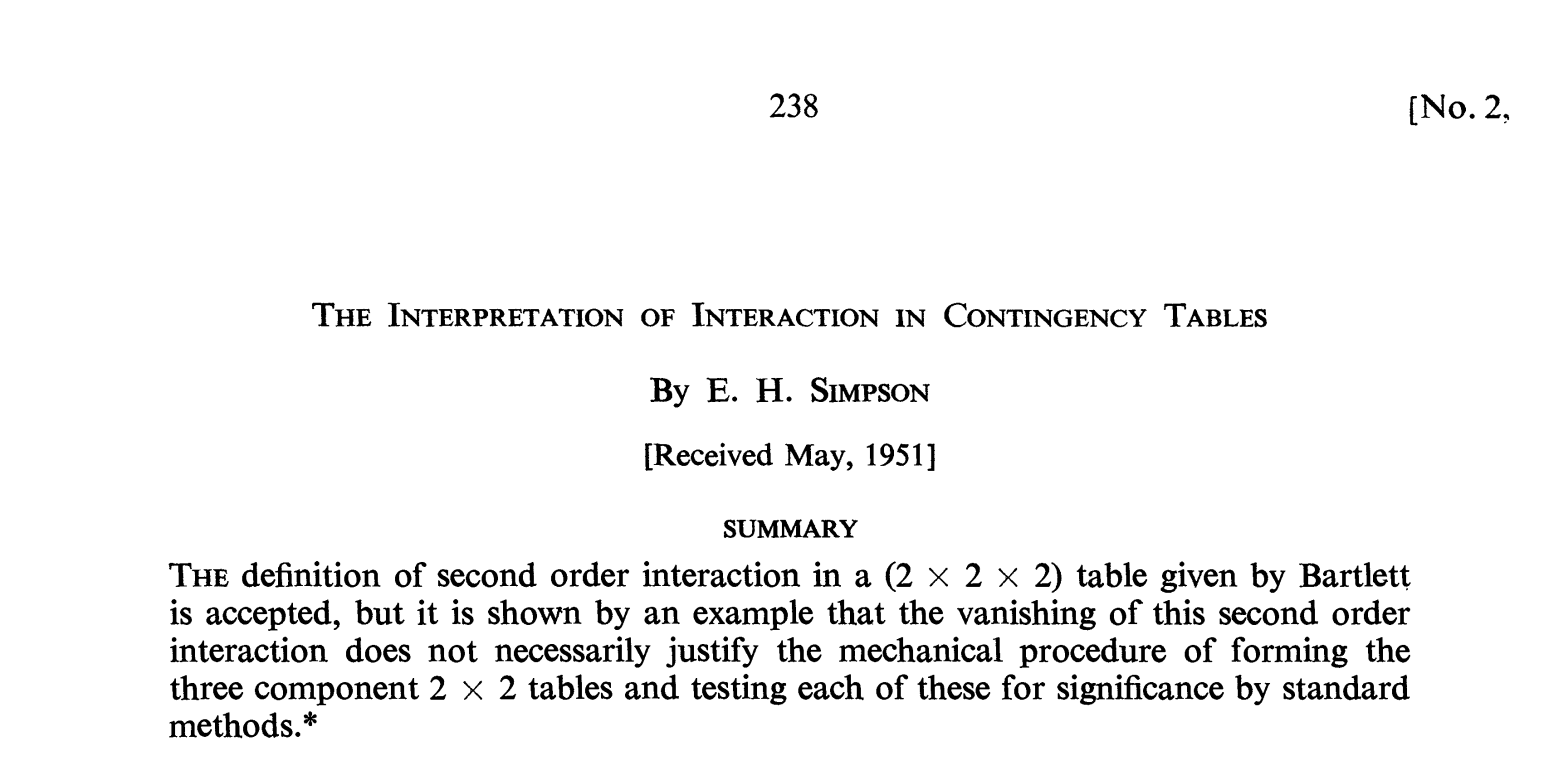
\includegraphics[width=\textwidth]{figs/lit-sim-1.png}
    \caption{Simpson, Edward H. (1951). "The Interpretation of Interaction in Contingency Tables". Journal of the Royal Statistical Society, Series B. 13: 238–241.}
\end{figure}

\end{frame}

\begin{frame}{Simpson's paradox -- origin}
\begin{figure}
    \centering
   
\includegraphics[width=\textwidth]{figs/lit-sim-2.png}
    \caption{Colin R. Blyth (June 1972). "On Simpson's Paradox and the Sure-Thing Principle". Journal of the American Statistical Association. 67 (338): 364–366}
\end{figure}
        
\end{frame}

\begin{frame}{UC Berkeley gender bias}
\begin{table}
\centering
\caption{A study of gender bias among graduate school admissions to the Uni\-ver\-si\-ty of California, Berkeley in 1973}
\scriptsize
\begin{tabular}{crrrrrr}
\hline
& \multicolumn{2}{c}{All} & \multicolumn{2}{c}{Men} & \multicolumn{2}{c}{Women} \\ 
& Applicants & Admitted
& Applicants & Admitted
& Applicants & Admitted \\
\hline
\text{Total} & 12,763 & 41\% & 8,442 & \alert{44\%} & 4,321 & 35\% \\
\hline
\end{tabular}
\begin{flushleft}
Source: \url{https://en.wikipedia.org/wiki/Simpsons_paradox}
\end{flushleft}
\end{table}
\end{frame}

\begin{frame}{UC Berkeley gender bias}
   \begin{table}[h]
\centering
\caption{A study of gender bias among graduate school admissions to the Uni\-ver\-si\-ty of California, Berkeley in 1973 -- the data from the six largest departments}
\scriptsize
\begin{tabular}{crrrrrr}
\hline
Department & \multicolumn{2}{c}{All} & \multicolumn{2}{c}{Men} & \multicolumn{2}{c}{Women} \\ 
& Applicants & Admitted
& Applicants & Admitted
& Applicants & Admitted \\
\hline
\text{A} & 933 & 64\% & {825} & 62\% & 108 & \alert{82\%} \\
\hline
\text{B} & 585 & 63\% & {560} & 63\% & 25 & \alert{68\%} \\
\hline
\text{C} & 918 & 35\% & 325 & \alert{37\%} & 593 & 34\% \\
\hline
\text{D} & 792 & 34\% & 417 & 33\% & 375 & \alert{35\%} \\
\hline
\text{E} & 584 & 25\% & 191 & \alert{28\%} & 393 & 24\% \\
\hline
\text{F} & 714 & 6\% & 373 & 6\% & 341 & \alert{7\%} \\
\hline
\text{Total} & \textbf{4526} & \textbf{39\%} & \textbf{2691} & \textbf{45\%} & \textbf{1835} & \textbf{30\%} \\
\hline
\end{tabular}
\begin{flushleft}
Source: \url{https://en.wikipedia.org/wiki/Simpsons_paradox}
\end{flushleft}
\end{table} 
\end{frame}


\begin{frame}{Kidney stone treatment}
\begin{table}[h]
\caption{Comparison of he success rates of two treatments for kidney stones}
\centering
\begin{tabular}{lll}
\hline
Stone size / Treatment & Treatment A & Treatment B \\
\hline
Small stones & \alert{93\%} (81/87) & 87\% (234/270) \\
Large stones & \alert{73\%} (192/263) & 69\% (55/80) \\
\hline
Both & 78\% (273/350) & \alert{83\%} (289/350) \\
\hline
\end{tabular}
\begin{flushleft}

\small
The table below shows the success rates (the term success rate here actually means the success proportion) and numbers of treatments for treatments involving both small and large kidney stones, where Treatment A includes open surgical procedures and Treatment B includes closed surgical procedures. The numbers in parentheses indicate the number of success cases over the total size of the group.

\vspace{0.5cm}

Source: \url{https://en.wikipedia.org/wiki/Simpsons_paradox} and Julious \& Mullee (1994). Confounding and Simpson's paradox. Bmj, 309(6967), 1480-1481.
\end{flushleft}
\end{table}
\end{frame}

\begin{frame}{Simpson's paradox in regression}
    \begin{figure}
        \centering
        
\includegraphics[width=0.7\textwidth]{figs/fig-simps-1.png}
        \caption{Example of Simpson's paradox on simulated data}
    \end{figure}
\end{frame}

\begin{frame}{Simpson's paradox in regression}
    \begin{figure}
        \centering
        
\includegraphics[width=0.7\textwidth]{figs/fig-simps-2.png}
        \caption{Example of Simpson's paradox on simulated data}
    \end{figure}
\end{frame}



\begin{frame}{Simpson's paradox -- causal perspective}

The paradox arises due to a \textbf{confounding variable} $Z$ that influences both the treatment/exposure $X$ and the outcome $Y$.

\vspace{0.5cm}

\begin{center}
\begin{tikzpicture}[node distance=2.5cm, >=stealth, thick]
    \node (Z) {$Z$ (confounder)};
    \node (X) [below left of=Z] {$X$ (exposure)};
    \node (Y) [below right of=Z] {$Y$ (outcome)};
    \draw[->] (Z) -- (X);
    \draw[->] (Z) -- (Y);
    \draw[->] (X) -- (Y);
\end{tikzpicture}
\end{center}

\vspace{0.5cm}

\begin{itemize}
    \item In the Berkeley example: $Z$ = department, $X$ = gender, $Y$ = admission.
    \item In the kidney stone example: $Z$ = stone size, $X$ = treatment, $Y$ = success.
    \item The marginal association between $X$ and $Y$ can reverse once we condition on $Z$.
    \item Key question: should we condition on $Z$? The answer depends on the \textbf{causal structure}, not just the data.
\end{itemize}

\end{frame}

\begin{frame}{}
\begin{center}
    
\includegraphics[width=0.4\textwidth]{figs/bookwhy.png}
\end{center}
\end{frame}

\begin{frame}{}
\begin{center}
    
\includegraphics[width=0.6\textwidth]{figs/scott1.png}
\end{center}
\end{frame}

\begin{frame}{}
\begin{center}
    
\includegraphics[width=0.7\textwidth]{figs/scott2.png}
\end{center}
\end{frame}



\begin{frame}{Literature}
    \begin{itemize}
    \justifying
        \item Simpson, Edward H. (1951). "The Interpretation of Interaction in Contingency Tables". Journal of the Royal Statistical Society, Series B. 13: 238–241.
        \item Pearson, Karl; Lee, Alice; Bramley-Moore, Lesley (1899). "Genetic (reproductive) selection: Inheritance of fertility in man, and of fecundity in thoroughbred racehorses". Philosophical Transactions of the Royal Society A. 192: 257–330. doi:10.1098/rsta.1899.0006
        \item G. U. Yule (1903). "Notes on the Theory of Association of Attributes in Statistics". Biometrika. 2 (2): 121–134. doi:10.1093/biomet/2.2.121.
        \item Colin R. Blyth (June 1972). "On Simpson's Paradox and the Sure-Thing Principle". Journal of the American Statistical Association. 67 (338): 364–366. doi:10.2307/2284382. JSTOR 2284382.
        \item Pearl, J. (2009). \textit{Causality: Models, Reasoning, and Inference}. Cambridge University Press.
    \end{itemize}
\end{frame}



\subsection{Measuring associations}
\begin{frame}{Contingency tables -- $\chi^2$ statistic}

\begin{itemize}
    \item In practice, the most popular way to verify if two variables ($X,Y$) are associated is to apply $\chi^2$ test (independence test). Hypotheses are as follows
    
    \begin{itemize}
        \item[H0:] variables ($X,Y$) are independent,
        \item[H1:] variables ($X,Y$) are dependent,
    \end{itemize}
    and the test statistic is given by
\begin{equation}
    \chi^{2}=\sum_{i=1}^{I} \sum_{j=1}^{J} \frac{\left(n_{i j}-\hat{n}_{i j}\right)^{2}}{\hat{n}_{i j}} \sim \chi^2((I-1)(J-1)).
\end{equation}

where $n_{ij}$ and $\hat{n}_{i j}$ are observed and expected counts respectively.
\item Expected (theoretical) counts are calculated according to

\begin{equation}
    \hat{n}_{i j}=\frac{n_{i .} n_{ . j}}{n}.
\end{equation}


\end{itemize}


\end{frame}

\begin{frame}{Contingency tables -- $\chi^2$ and $G^2$ statistic}

For tables with small frequencies a continuity correction should be applied.

\begin{equation}
    \chi_{\mathrm{Yates}}^{2}=\sum_{i=1}^{I}\sum_{j=1}^J \frac{\left(\left|n_{ij}-\hat{n}_{ij}\right|-0.5\right)^{2}}{\hat{n}_{ij}}.
\end{equation}

Log-likelihood $G^2$ statistic

\begin{equation}
    G^{2}=2 \sum_{i=1}^{I} \sum_{j=1}^{J} n_{i j} \log \left(\frac{n_{i j}}{\hat{n}_{i j}}\right),
\end{equation}

\noindent $\log$ refers to the natural logarithm.
\end{frame}

\begin{frame}{Contingency tables -- Fisher's exact test}

\begin{itemize}
    \item For $2 \times 2$ tables with small expected counts (e.g. $\hat{n}_{ij} < 5$), even Yates' correction may be insufficient. Fisher's exact test provides an \textbf{exact} $p$-value.

    \item Under $H_0$ of independence, conditioning on both row and column marginals, the cell count $n_{11}$ follows a hypergeometric distribution:

\begin{equation}
    P(n_{11} = x) = \frac{\binom{n_{1.}}{x}\binom{n_{2.}}{n_{.1}-x}}{\binom{n}{n_{.1}}}.
\end{equation}

    \item The $p$-value is computed by summing probabilities over all tables as extreme or more extreme than the observed one.

    \item No asymptotic approximation is involved -- the test is valid for \textbf{any} sample size.

    \item Extensions to $r \times c$ tables exist but become computationally intensive (e.g. Freeman-Halton test).
\end{itemize}

\end{frame}



\begin{frame}{When $\chi^2$ approximation fails -- example}

\begin{table}[h]
\centering
\caption{A hypothetical $2 \times 2$ table with small expected counts (left) and testing results (right)}
\small
\begin{tabular}{lccc}
\hline
 & Success & Failure & Total \\
\hline
Treatment & 1 & 9 & 10 \\
Control   & 5 & 5 & 10 \\
\hline
Total     & 6 & 14 & 20 \\
\hline
\end{tabular}
%
\hspace{1cm}
\begin{tabular}{lcc}
\hline
Test & Statistic & $p$-value \\
\hline
Pearson $\chi^2$ & 3.810 & 0.051 \\
$\chi^2_{\text{Yates}}$ & 2.143 & 0.143 \\
$G^2$ & 4.011 & 0.045 \\
Fisher's exact & -- & 0.141 \\
\hline
\end{tabular}
\end{table}

Expected counts: $\hat{n}_{11} = 3$, $\hat{n}_{12} = 7$, $\hat{n}_{21} = 3$, $\hat{n}_{22} = 7$.

\vspace{0.3cm}

\small
Pearson's $\chi^2$ is \textbf{anti-conservative} here -- its $p$-value is too small because the $\chi^2$ approximation is poor when expected counts are low. Yates' correction and Fisher's exact test give more appropriate (larger) $p$-values. The $G^2$ statistic is also anti-conservative in small samples.

\end{frame}


\begin{frame}{Contingency tables -- generalization}

Cressie-Read statistic (aka Power Divergence statistic)

\begin{equation}
    CR=\frac{2}{\lambda(\lambda+1)} \sum_{i=1}^{I} \sum_{j=1}^{J} n_{i j}\left[\left(\frac{n_{i j}}{\hat{n}_{i j}}\right)^{\lambda}-1\right].
\end{equation}

When $\lambda=1$ then we get $\chi^2$, if $\lambda \to 0$ then we get $G^{2}$. Cressie and Read (1984) suggested $\lambda=2/3$.

\vspace{0.5cm}

Literature: 
\begin{itemize}
    \small
    \item Cressie \& Read (1984). Multinomial goodness‐of‐fit tests. Journal of the Royal Statistical Society: Series B (Methodological), 46(3), 440-464.
    \item Cressie \& Read (1989). Pearson's X2 and the log-likelihood ratio statistic G2: a comparative review. International Statistical Review, 19-43.
\end{itemize}
\end{frame}

\begin{frame}{Contingency tables -- correlation}
    \begin{itemize}
        \item Yule's $\phi$, range: $[0,\infty)$
        \begin{equation}
            \Phi=\sqrt{\frac{\chi^{2}}{n}}
        \end{equation}
        \item Pearson's $C$, range: $[0,\infty)$
        \begin{equation}
            C=\sqrt{\frac{\chi^{2}}{\chi^{2}+n}}
        \end{equation}
        \item Chuprov's $T$, range: $[0,1]$
        \begin{equation}
            T=\sqrt{\frac{\chi^{2}}{n \sqrt{(I-1)(J-1)}}}
        \end{equation}
        \item Cramer's $V$, range: $[0,1]$
        \begin{equation}
            V=\sqrt{\frac{\chi^{2}}{n \cdot \min \{I-1, J-1\}}}
        \end{equation}
    \end{itemize}
\end{frame}

\begin{frame}{Literature (selected)}
    \begin{itemize}
        \item Fagerland, M., Lydersen, S., \& Laake, P. (2017). Statistical analysis of contingency tables. Chapman and Hall/CRC. see \url{https://contingencytables.com/software-resources}
    \end{itemize}
\end{frame}
\begin{frame}{Practice -- contingency tables}
      \begin{table}[]
        \centering
        \caption{Overview of functions}
        %\label{tab:my_label}
        \begin{tabular}{cp{3cm}p{3cm}p{3cm}}
        \hline
          \textbf{Language}   & \textbf{R} &  \textbf{Python} & \textbf{Julia} \\
        \hline
         Packages  & 
         stats, vcd & scipy.stats, pingouin &  Hypothesis\-Tests.jl \\
        Functions &
          xtabs(), table(); assocstats() & chi\_contingency()  & Power\-Divergence\-Test() \\
        \hline
        \end{tabular}
 
    \end{table}
\end{frame}

\section{Discrete distributions}

\begin{frame}{}
\begin{center}
    \Large{Discrete distributions}
\end{center}    
\end{frame}


\subsection{Theory}

\begin{frame}{Discrete Statistical Distributions}

\begin{itemize}
    \item \textbf{Probability Mass/Density Function} -- The probability mass function of a random variable $X$ is defined as the probability that the random variable takes on a particular value.
        \begin{equation}
            p \left( x _ { k } \right) = P \left[ X = x _ { k } \right]
        \end{equation}
    \item \textbf{Cumulative Distribution Function} -- The cumulative distribution function is
    
    \begin{equation}
        F ( x ) = P [ X \leq x ] = \sum _ { x _ { k } \leq x } p \left( x _ { k } \right)
    \end{equation}
\end{itemize}    
\end{frame}


\begin{frame}[fragile]{Discrete distributions}

During the lecture we will discuss the following distributions

\begin{itemize}
    \item univariate
    
    \begin{itemize}
        \item Bernoulli distribution
        \item Binomial distribution
        \item Geometric distribution
        \item Negative binomial distribution
        \item Poisson distribution
    \end{itemize}
    \item multivariate
    
        \begin{itemize}
        \item Multinomial distribution 
    \end{itemize}
    
    \end{itemize}

For more information see the following links


\begin{itemize}
    \item \href{https://en.wikipedia.org/wiki/List_of_probability_distributions#Discrete_distributions}{Distributions (Wikipedia)}
    \item \href{https://cran.r-project.org/web/views/Distributions.html}{R CRAN Task View: Probability Distributions} 
    \item \href{https://docs.scipy.org/doc/scipy/reference/stats.html}{Python Statistical functions (scipy.stats)} 
    \item \href{https://juliastats.github.io/Distributions.jl/stable/}{Julia Distributions.jl Package}
\end{itemize}
\end{frame}


%%%%%%%%%%%% Bernoulli %%%%%%%%%%%%%%%%%%

\begin{frame}{Bernoulli distribution}
    A Bernoulli distribution is parameterized by a success rate $p$, which takes value $1$ with probability $p$ and $0$ with probability $1-p$

\begin{equation}
    P(X = k) = \begin{cases}
1 - p & \quad \text{for } k = 0, \\
p & \quad \text{for } k = 1.
\end{cases}
\end{equation}

We can denote this distribution as $X \sim \mathrm{Bernoulli}(p)$.

\vspace{0.5cm}

\textbf{Example}: a (single) coin toss.

\end{frame}

\begin{frame}{Bernoulli distribution -- properties}

\begin{itemize}
    \item Expected value 
        \begin{equation}
            E(X) = p
        \end{equation}
    \item Variance
            \begin{equation}
            V(X) = p(1-p) = pq
        \end{equation}
    \item Skewness
            \begin{equation}
            Skew(X) = \frac{q-p}{\sqrt{pq}} = \frac{1-2p}{\sqrt{pq}}
        \end{equation}
\end{itemize}
\end{frame}

%%%%%%%%%%%% Binomial %%%%%%%%%%%%%%%%%%

\begin{frame}{Binomial distribution}
    A Binomial distribution characterizes the number of successes in a sequence of independent trials. It has two parameters: $n$, the number of trials, and $p$, the probability of success in an individual trial, with the distribution:
    
    \begin{equation}
        P(X = k) = {n \choose k}p^k(1-p)^{n-k},  \quad \text{ for } k = 0,1,2, \ldots, n.
    \end{equation}

We can denote this distribution as $X \sim \mathrm{B}(n,p)$.

\vspace{0.5cm}

\textbf{Example}: multiple, independent, coin toss.


\end{frame}

\begin{frame}{Binomial distribution}

\begin{figure}
    \centering
    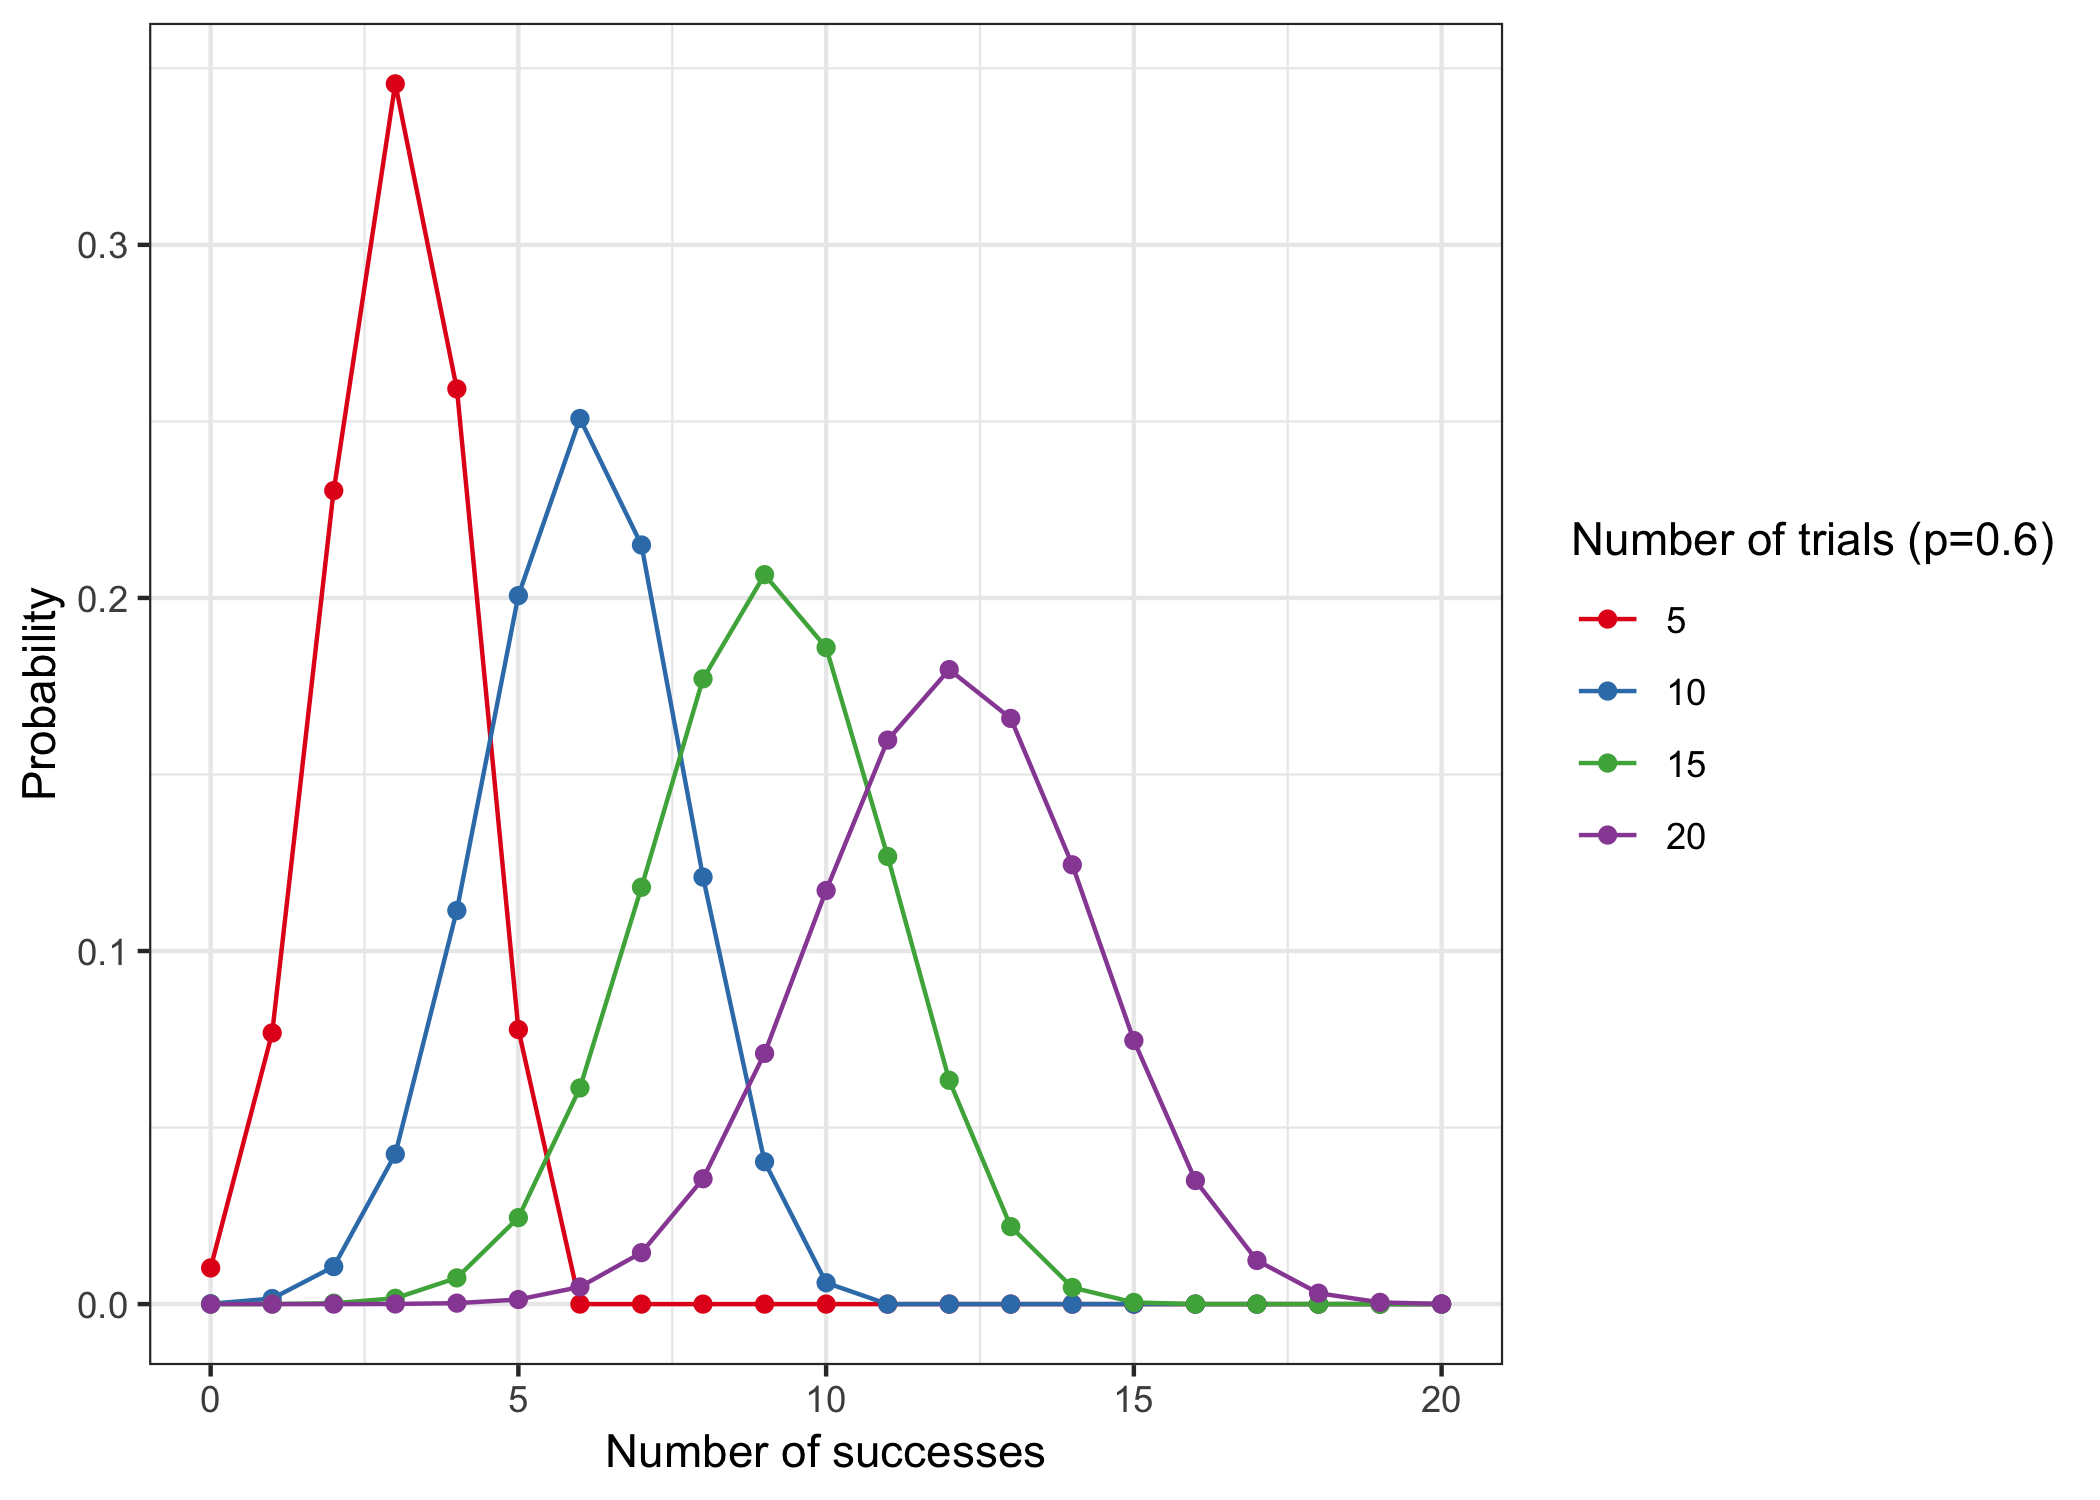
\includegraphics[width=0.7\textwidth]{figs/binomial_example.png}
    \caption{Probability mass function (PMF) of the binomial distribution}
\end{figure}

\end{frame}

\begin{frame}{Binomial distribution -- properties}

\begin{itemize}
    \item Expected value 
        \begin{equation}
            E(X) = np
        \end{equation}
    \item Variance
            \begin{equation}
            V(X) = np(1-p) = npq
        \end{equation}
\end{itemize}
\end{frame}

%%%%%%%%%%%% Geometric %%%%%%%%%%%%%%%%%%

\begin{frame}{Geometric distribution}
    A Geometric distribution characterizes the number of trials until the first success in a sequence of independent Bernoulli trials with success rate $p \in (0,1]$
    
    \begin{equation}
        P(X = k) = p (1 - p)^{k-1}, \quad \text{for } k = 1, 2, 3, \ldots.
    \end{equation}

We can denote this distribution as $X \sim \mathrm{G}(p)$.


\vspace{0.5cm}

\textbf{Example}: throwing a die until 6 appears. 



\end{frame}


\begin{frame}{Geometric distribution}

\begin{figure}
    \centering
    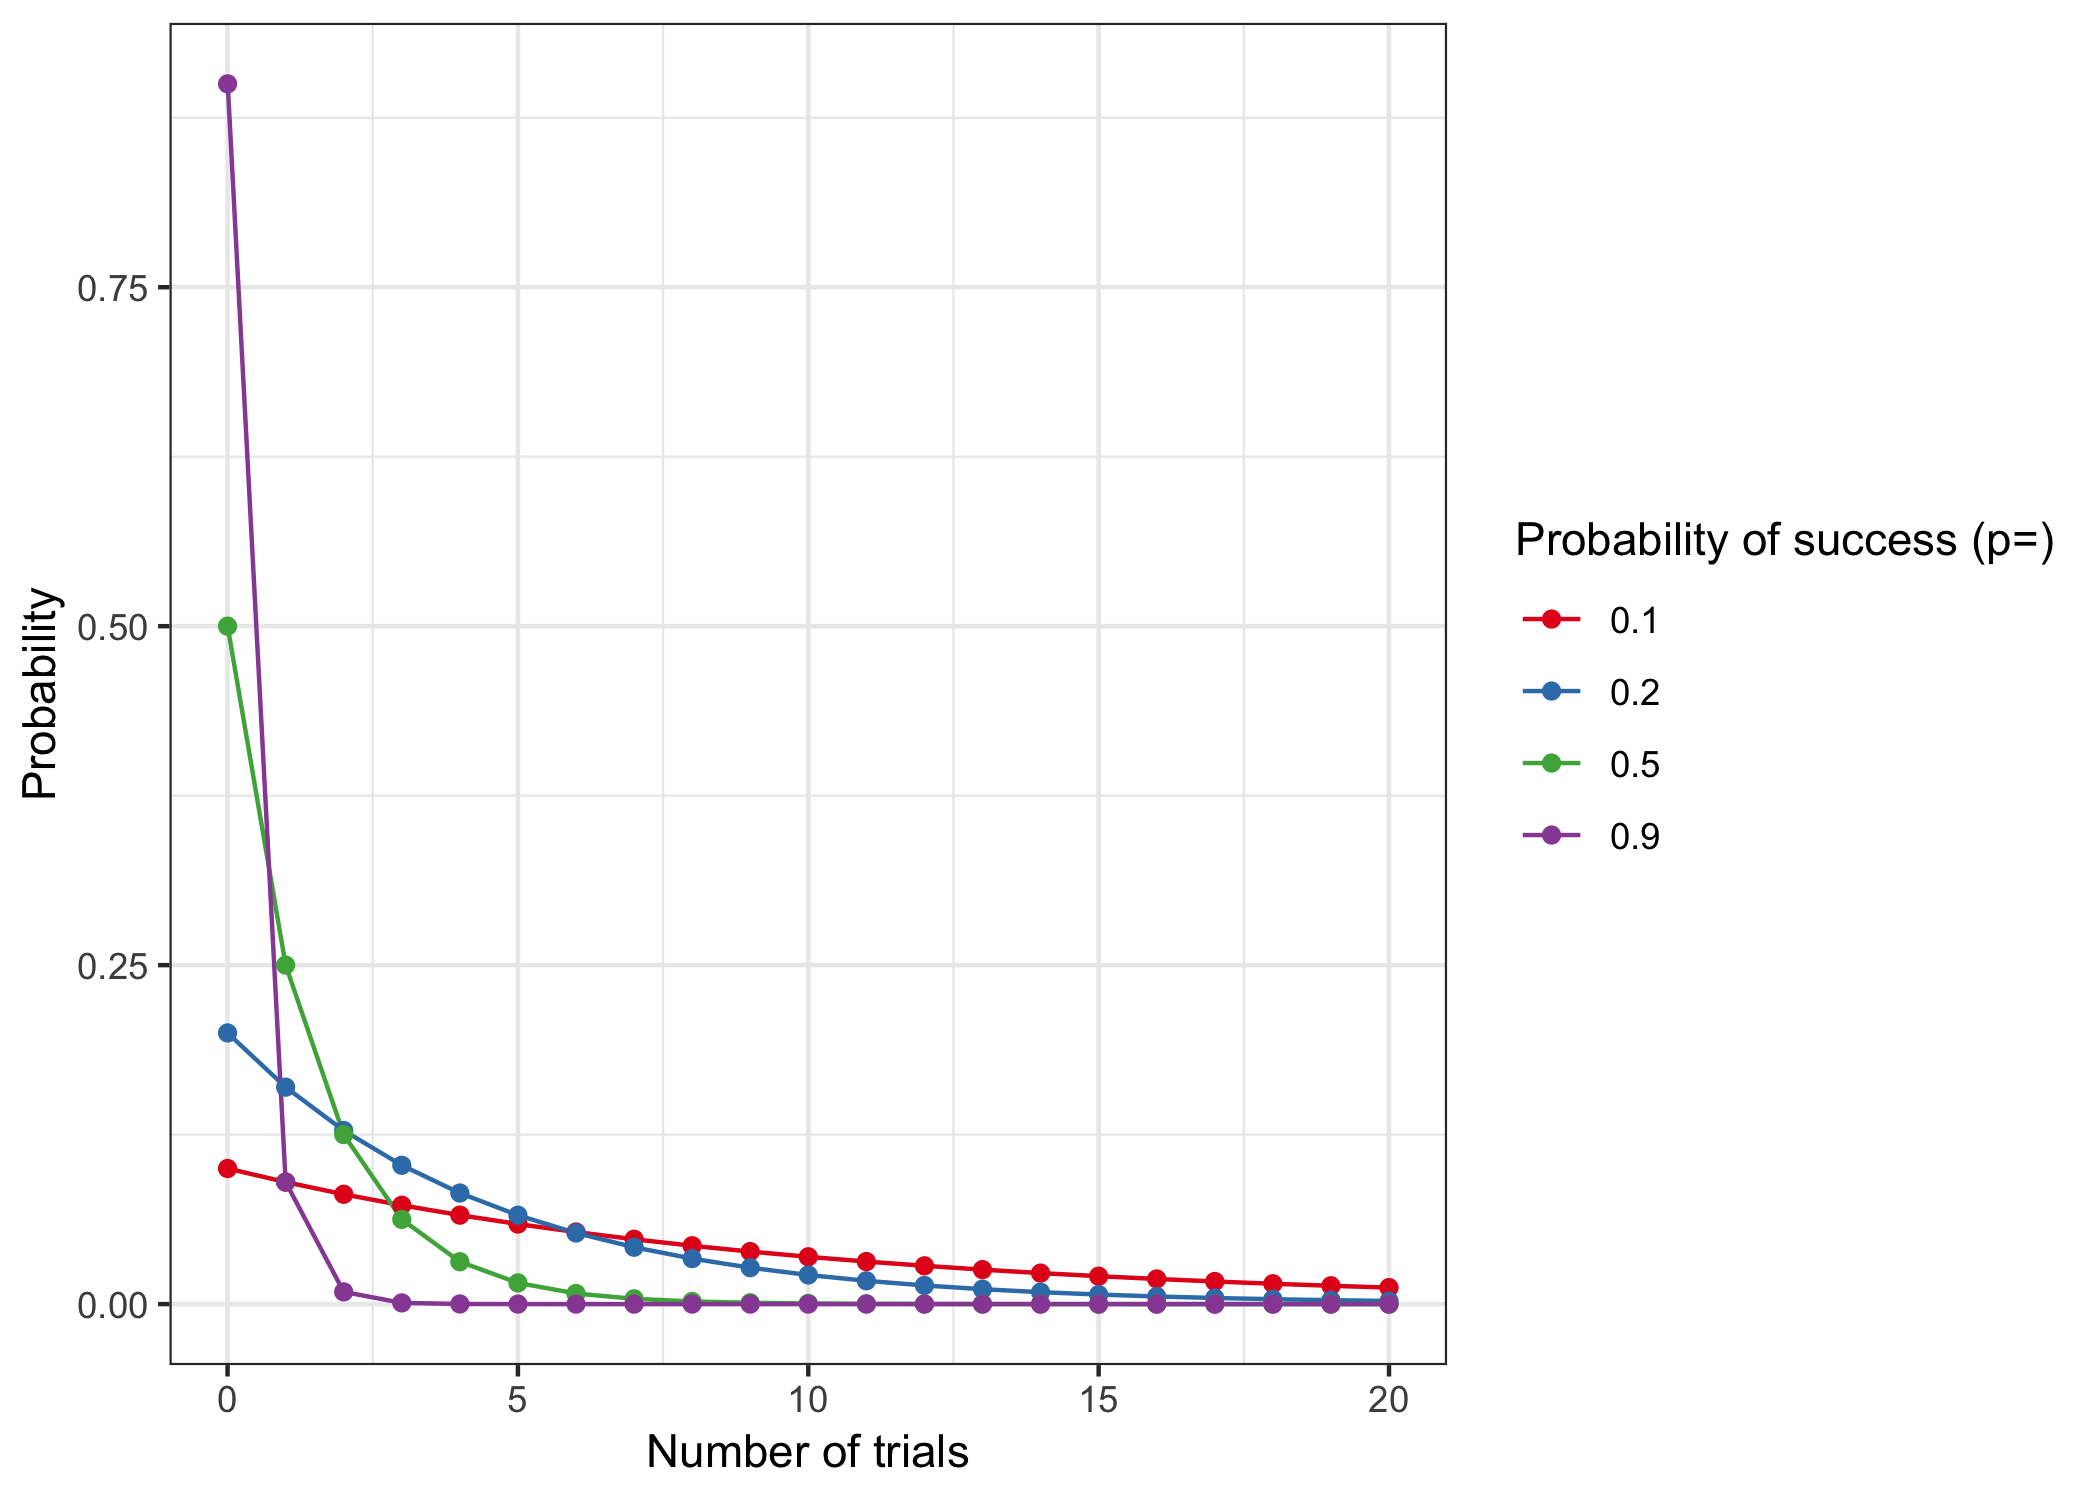
\includegraphics[width=0.7\textwidth]{figs/geometric_example.png}
    \caption{Probability mass function (PMF) of the geometric distribution}
\end{figure}

\end{frame}

\begin{frame}{Geometric distribution -- properties}

\begin{itemize}
    \item Expected value 
        \begin{equation}
            E(X) = \frac{1}{p}
        \end{equation}
    \item Variance
            \begin{equation}
            V(X) = \frac{1-p}{p^2}
        \end{equation}
\end{itemize}
\end{frame}

%%%%%%%%%%%% Negative binomial %%%%%%%%%%%%%%%%%%


\begin{frame}{Negative binomial (Pascal) distribution}
    A Negative binomial distribution describes the number of failures before the $r$th success in a sequence of independent Bernoulli trials. It is parameterized by $r$, the number of successes, and $p$, the probability of success in an individual trial.
    
    \begin{equation}
        P(X = k) = {k + r - 1 \choose k} p^r (1 - p)^k, \quad \text{for } k = 0,1,2,\ldots.
\end{equation}
    
    The distribution remains well-defined for any positive $r$, in which case
     
\begin{equation}
        P(X = k) = \frac{\Gamma(k+r)}{k! \Gamma(r)} p^r (1 - p)^k, \quad \text{for } k = 0,1,2,\ldots.
\end{equation}


We can denote this distribution as $X \sim \mathrm{NB}(r,p)$.

\vspace{0.5cm}

\textbf{Example}: For example, we can define rolling a 6 on a dice as a success, and rolling any other number as a failure, and ask how many failure rolls will occur before we see the third success (r=3).
\end{frame}

\begin{frame}{Negative Binomial: Mean and Size Parameterization}
    An alternative parameterization uses the mean $\mu$ and size $\theta$ (dispersion parameter):
    \[
    p = \frac{\theta}{\theta + \mu}, \quad \text{where } r = \theta
    \]
    \textbf{Mean and Variance:}
    \[
    E(X) = \mu, \quad \text{Var}(X) = \mu + \frac{\mu^2}{\theta}
    \]

    \textbf{PMF:}
    \[
    P(X = k) = \binom{k + \theta - 1}{k} \left(\frac{\theta}{\theta + \mu}\right)^\theta \left(\frac{\mu}{\theta + \mu}\right)^k, \quad k = 0, 1, \ldots
    \]

    \vspace{0.3cm}

    \textbf{Example}: Rolling a 6 ($p = 1/6$), $r = 3$ in standard form.
    \begin{itemize}
    \scriptsize
        \item Standard: $\mu = \frac{3 (1 - 1/6)}{1/6} = 15$, $\theta = r = 3$
        \item Variance: $\mu + \frac{\mu^2}{\theta} = 15 + \frac{15^2}{3} = 15 + 75 = 90$
        \item Check: $p = \frac{3}{3 + 15} = \frac{3}{18} = \frac{1}{6}$
        \item $P(X = 7) = \binom{9}{7} \left(\frac{3}{18}\right)^3 \left(\frac{15}{18}\right)^7 \approx 0.043$
    \end{itemize}

    Larger $\theta$ reduces variance toward $\mu$ (Poisson-like)!
\end{frame}

\begin{frame}{Negative binomial (Pascal) distribution}

\begin{figure}
    \centering
    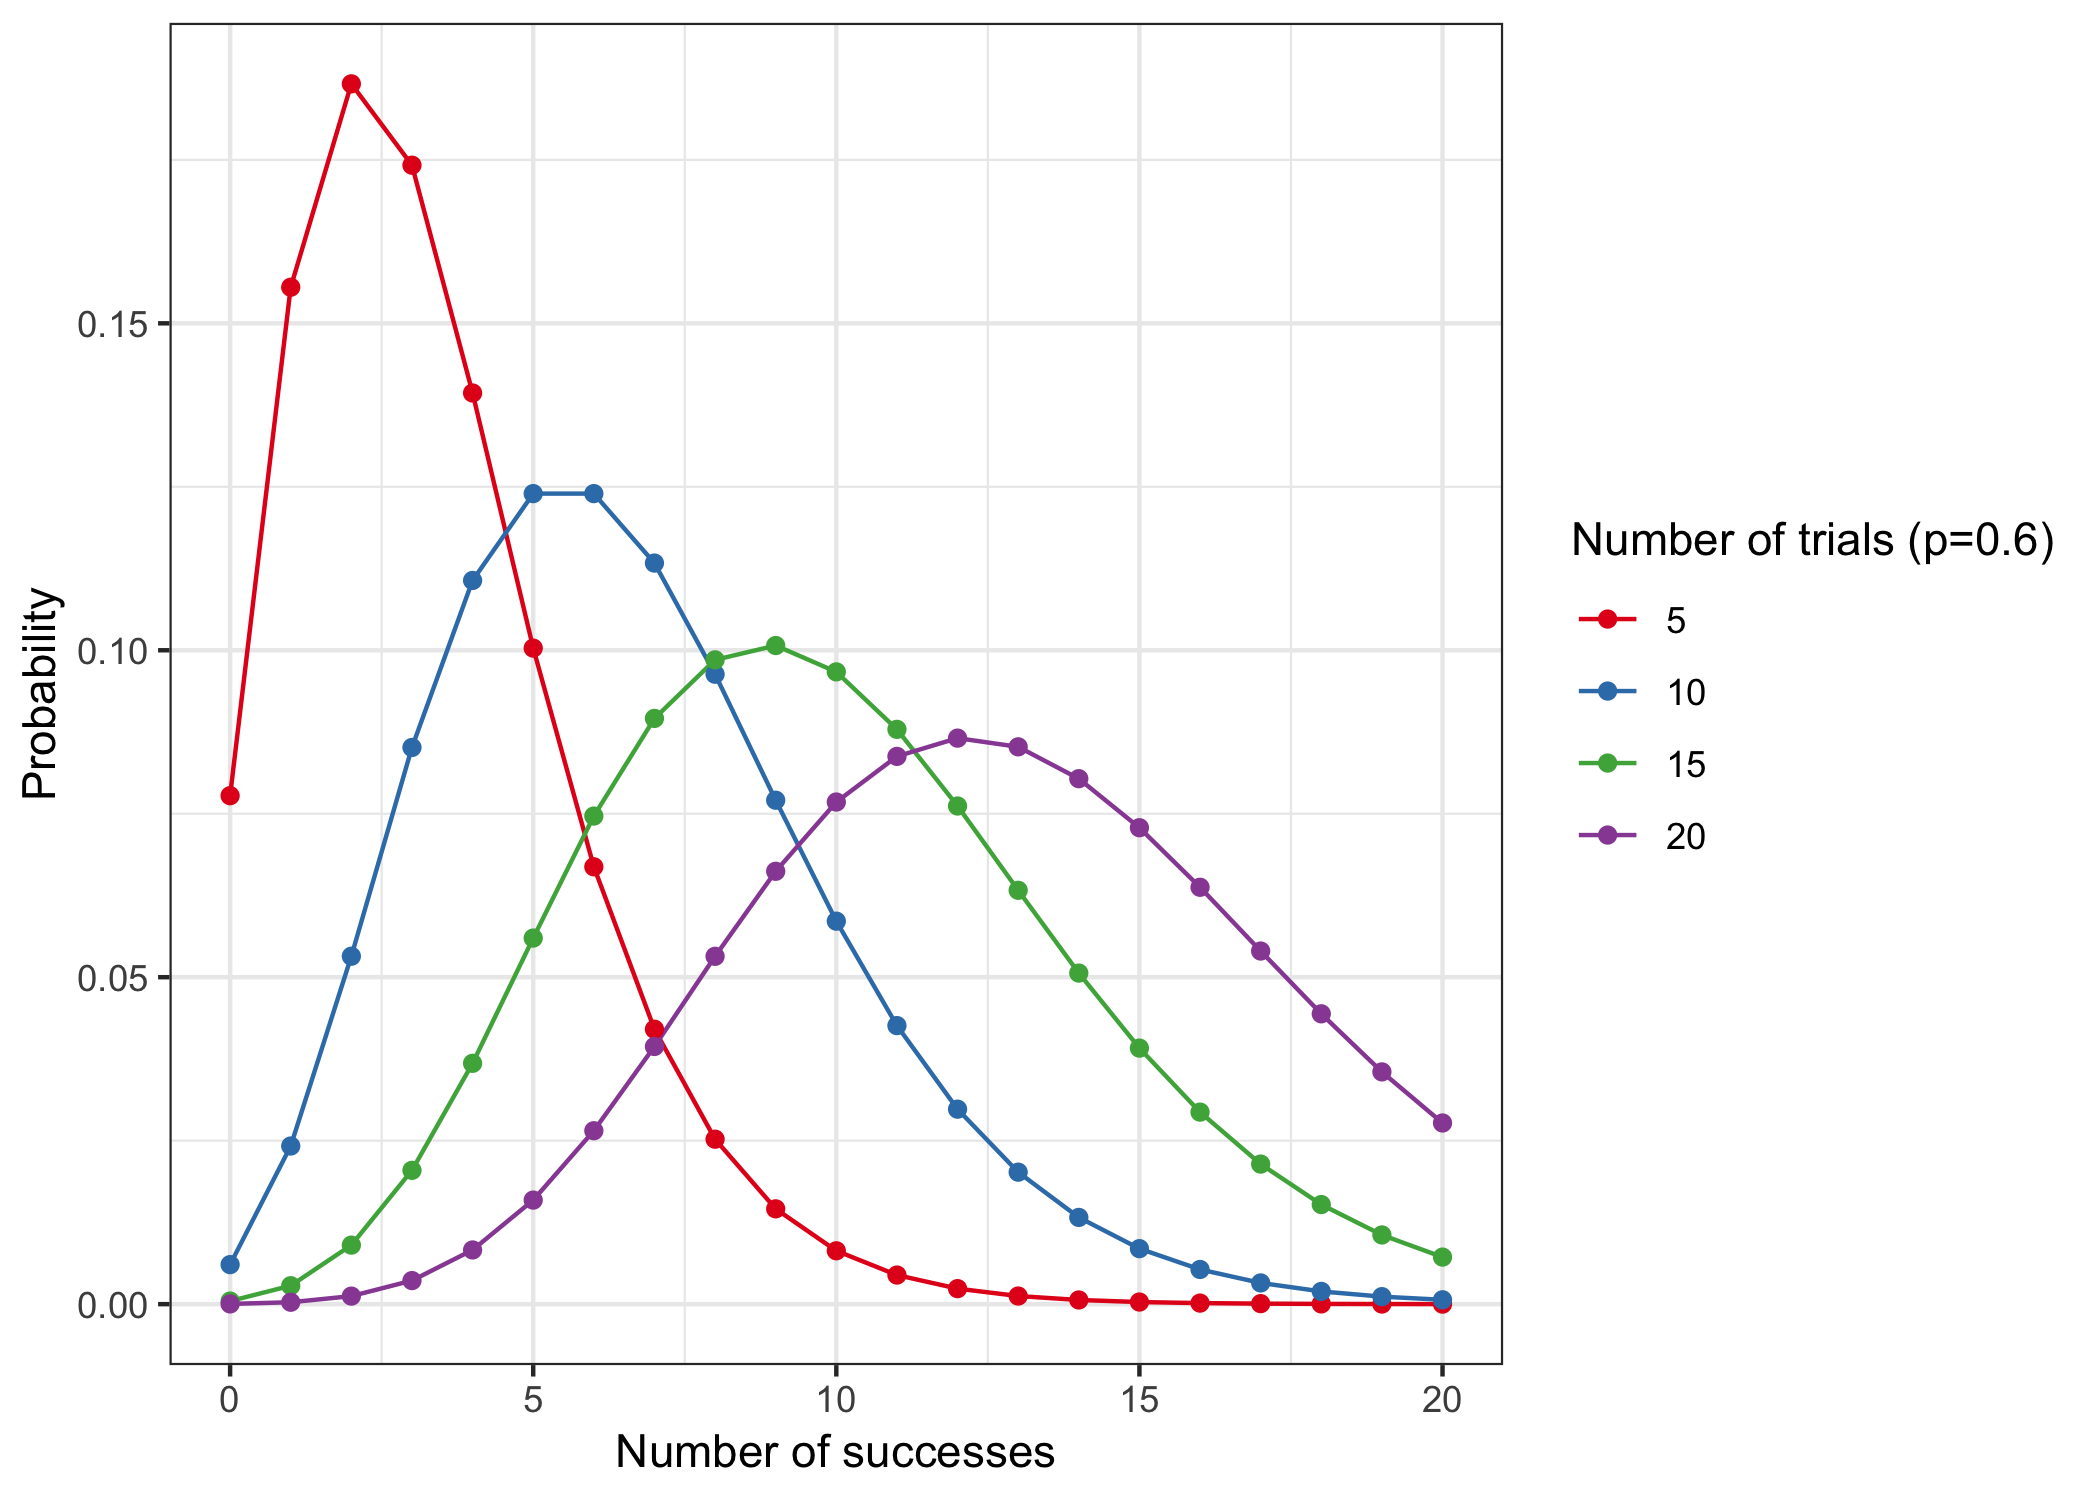
\includegraphics[width=0.7\textwidth]{figs/nbinomial_example.png}
    \caption{Probability mass function (PMF) of the negative binomial distribution}
\end{figure}

\end{frame}


\begin{frame}{Negative binomial (Pascal) distribution -- properties}

\begin{itemize}
    \item Expected value 
        \begin{equation}
            E(X) = \frac{r(1-p)}{p}
        \end{equation}
    \item Variance
            \begin{equation}
            V(X) = \frac{r(1-p)}{p^2}
        \end{equation}
\end{itemize}
\end{frame}


%%%%%%%%%%%% Poisson %%%%%%%%%%%%%%%%%%

\begin{frame}{Poisson distribution}
    A Poisson distribution describes the number of independent events occurring within a unit time interval, given the average rate of occurrence $\lambda$.
    
    \begin{equation}
        P(X = k) = \frac{\lambda^k}{k!} e^{-\lambda}, \quad \text{ for } k = 0,1,2,\ldots.
    \end{equation}
 
 We can denote this distribution as $X \sim \mathrm{Po}(\lambda)$ or $X \sim \mathrm{Pois}(\lambda)$.

  
  \vspace{0.5cm}

\textbf{Example}: Number of patients in the clinic.
  
\end{frame}

\begin{frame}{Poisson distribution}

\begin{figure}
    \centering
    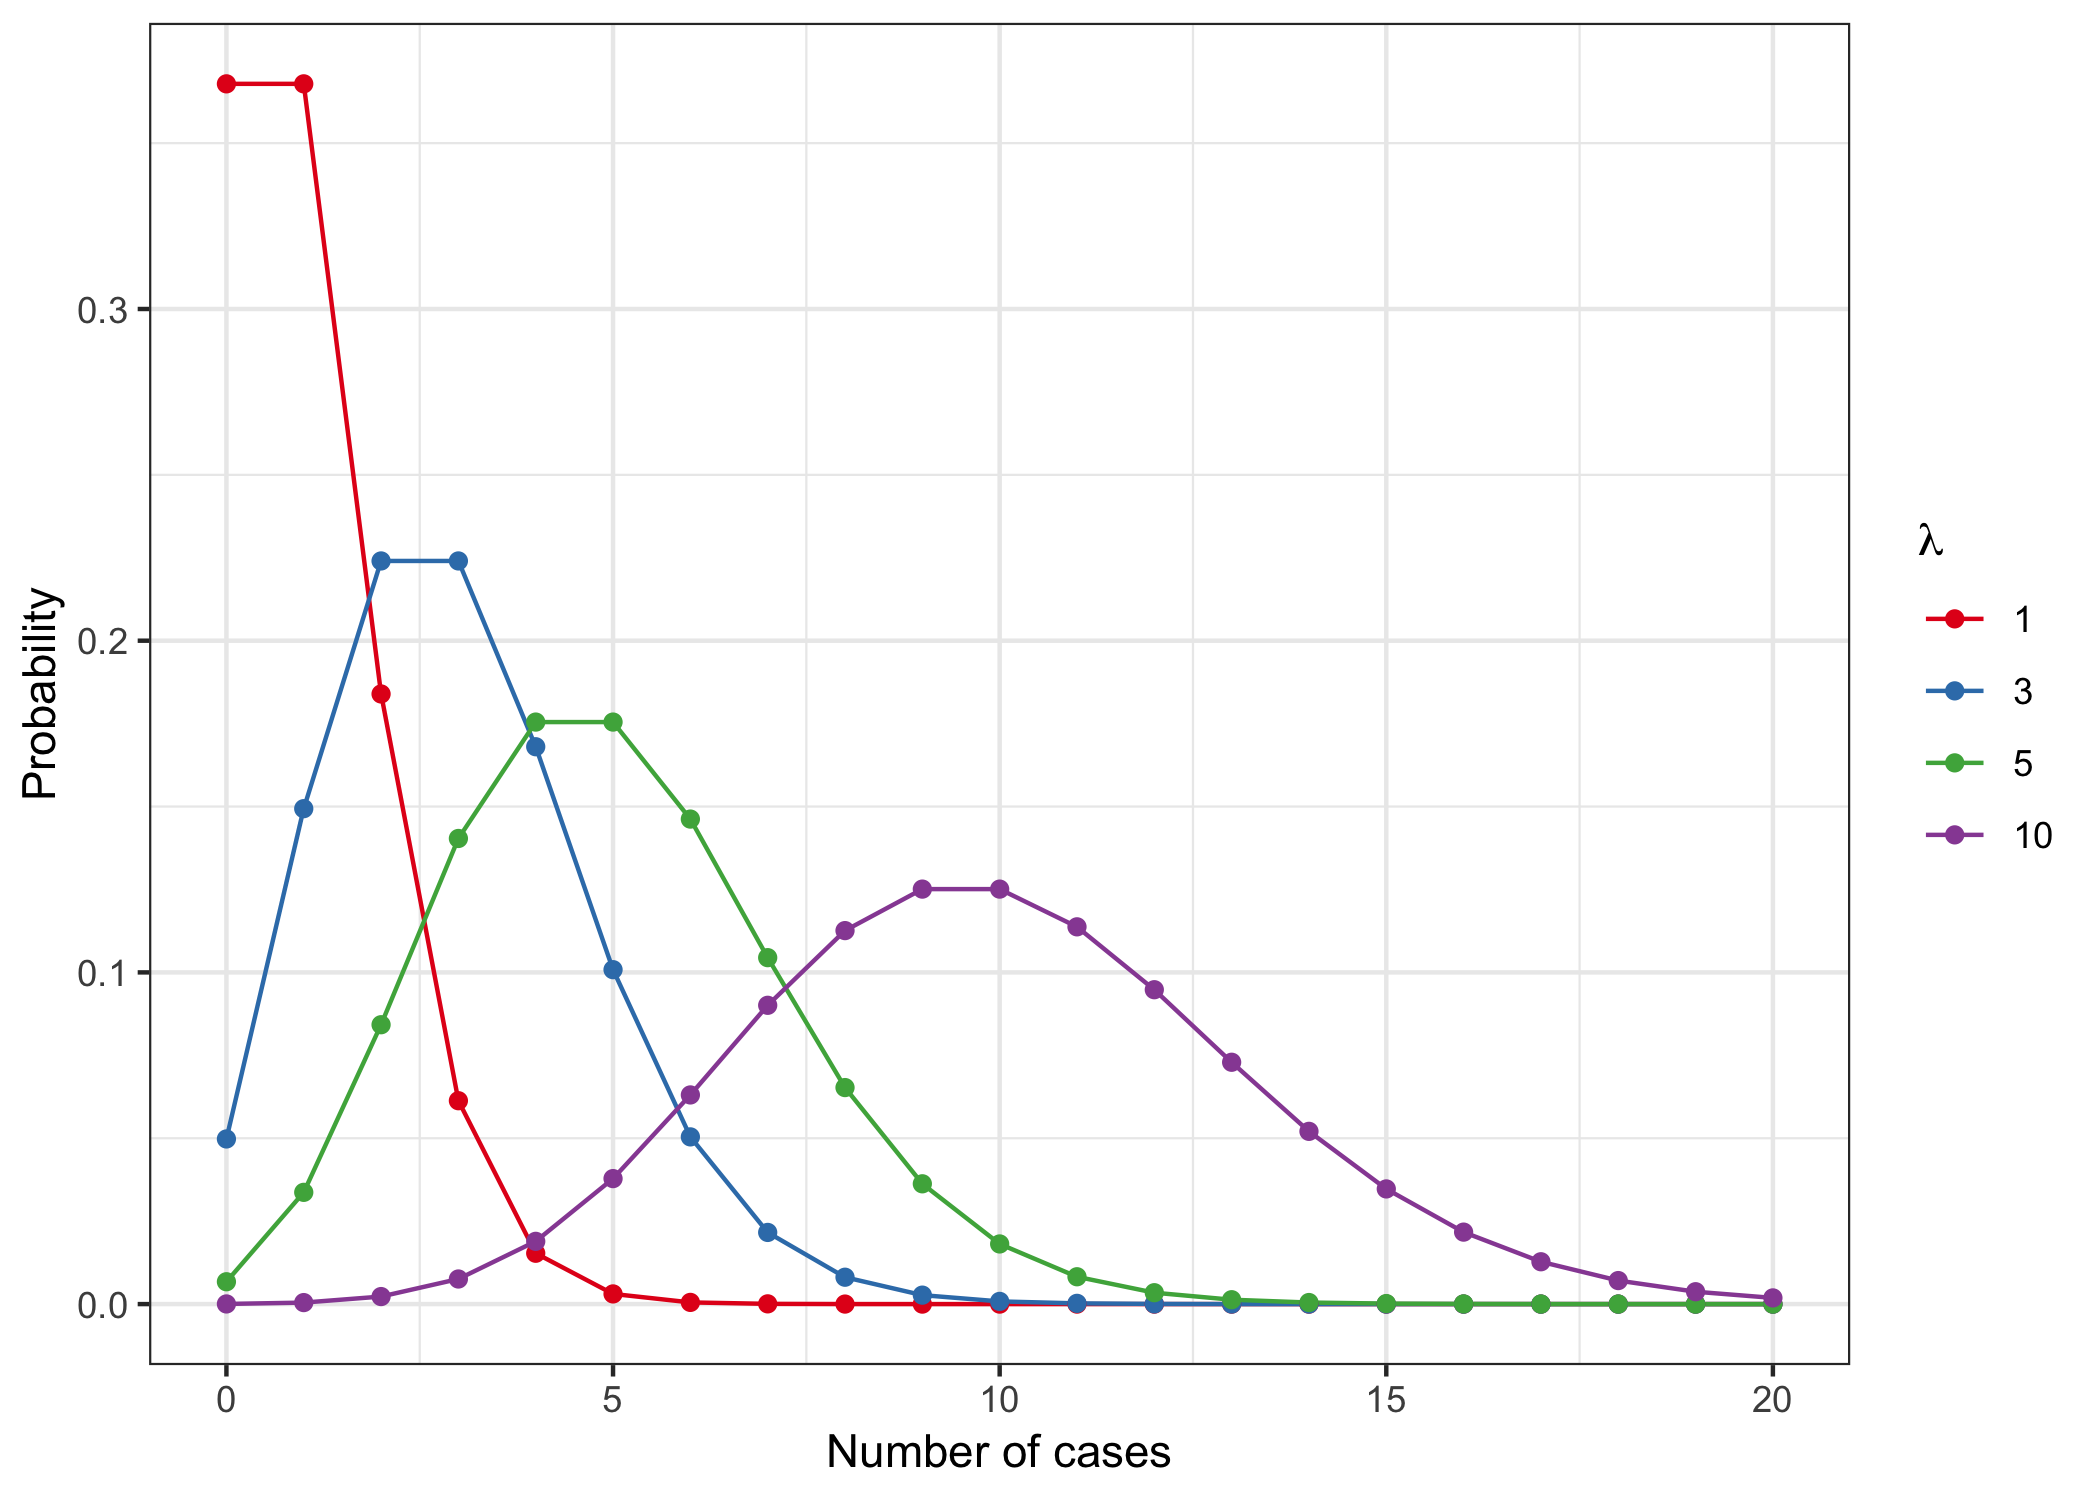
\includegraphics[width=0.7\textwidth]{figs/poisson_example.png}
    \caption{Probability mass function (PMF) of the Poisson distribution}
\end{figure}

\end{frame}


\begin{frame}{Poisson distribution -- properties}

\begin{itemize}
    \item Expected value 
        \begin{equation}
            E(X) = \lambda
        \end{equation}
    \item Variance
            \begin{equation}
            V(X) = \lambda
        \end{equation}
\end{itemize}
\end{frame}

\begin{frame}{Overdispersion and underdispersion}

The \textbf{dispersion index} is defined as
\begin{equation}
    D = \frac{\text{Var}(X)}{E(X)}
\end{equation}

\begin{itemize}
    \item \textbf{Equidispersion} ($D = 1$): Poisson distribution assumes $\text{Var}(X) = E(X) = \lambda$
    \item \textbf{Overdispersion} ($D > 1$): $\text{Var}(X) > E(X)$ -- very common in real count data (e.g.\ heterogeneity across units, clustering)
    \item \textbf{Underdispersion} ($D < 1$): $\text{Var}(X) < E(X)$ -- less common
\end{itemize}

\vspace{0.3cm}

The Negative Binomial distribution naturally handles overdispersion:
\begin{equation}
    \text{Var}(X) = \mu + \frac{\mu^2}{\theta} > \mu = E(X)
\end{equation}

As $\theta \to \infty$, $\text{Var}(X) \to \mu$ and $\text{NB} \to \text{Poisson}$.

\end{frame}

%%%%%%%%%%%% Multinomial %%%%%%%%%%%%%%%%%%

\begin{frame}{Multinomial distribution}
    The Multinomial distribution generalizes the binomial distribution. Consider $n$ independent draws from a categorical distribution over a finite set of size $k$, and let $X=(X_1,...,X_k)$ where $X_i$ represents the number of times the element $i$ occurs, then the distribution of $X$ is a multinomial distribution. Each sample of a multinomial distribution is a $k$-dimensional integer vector that sums to $n$.
    
    \vspace{1cm}
    
    The probability mass function is given by

    \begin{equation}
        f(x; n, p) = \frac{n!}{x_1! \cdots x_k!} \prod_{i=1}^k p_i^{x_i},
\quad x_1 + \cdots + x_k = n
    \end{equation}

 We can denote this distribution as $X \sim \mathrm{Mult}(n, \pi)$

\vspace{0.2cm}

    \textbf{Example}: Labour market status (i.e. employed, unemployed, inactive).
  
\end{frame}


\begin{frame}{Multinomial distribution -- properties}

\begin{itemize}
    \item Expected value 
        \begin{equation}
            E \left\{ X _ { i } \right\} = n p _ { i }
        \end{equation}
    \item Variance and covariance
            \begin{equation}
            \operatorname { Var } \left( X _ { i } \right) = n p _ { i } \left( 1 - p _ { i } \right)
        \end{equation}
        \begin{equation}
           \operatorname { Cov } \left( X _ { i } , X _ { j } \right) = - n p _ { i } p _ { j } ( i \neq j )
        \end{equation}
\end{itemize}
\end{frame}


\begin{frame}{Relation between Poisson and Multinomial distribution}
Suppose that $X_1, X_2, ..., X_k$ are independent Poisson random variables ($X_k \sim Po(\lambda_k)$) where the $\lambda_j$ are not necessarily equal ($j \in 1:k)$. Then the conditional distribution of the vector

\begin{equation}
    X=(X_1,X_2,\ldots,X_k),
\end{equation}

given the total

\begin{equation}
    n=X_1+X_2+\ldots+X_k
\end{equation}
is $Mult(n, \pi),$  where

\begin{equation}
    \pi=(\pi_1,\pi_2,\ldots,\pi_k)
\end{equation}
and
\begin{equation}
    \pi_j=\dfrac{\lambda_j}{\lambda_1+\lambda_2+\cdots+\lambda_k}.
\end{equation}

\end{frame}

\begin{frame}{Poisson-Multinomial connection -- advanced example}

An advanced worked example demonstrating this relation using the Polish Job Vacancy Survey data (vacancies by NACE section) is available in the notebook.

\vspace{0.5cm}

\textbf{Idea}: If vacancies in each NACE section follow independent Poisson distributions, then conditional on the total number of vacancies, the allocation across sections follows a Multinomial distribution.

\end{frame}

%%%%%%%%%%%% relations %%%%%%%%%%%%%%%%%%

\begin{frame}[fragile]{Relations between distributions}

\begin{itemize}
    \item A binomial $(n, p)$ random variable with $n = 1$, is a Bernoulli ($p$) random variable.
    \item A negative binomial distribution with $n = 1$ is a geometric distribution.
    \item If $X$ is a binomial $(n, p)$ random variable and if $n$ is large and $np$ is small then $X$ approximately has a Poisson($\lambda=np$) distribution.
    \item If $X$ is a negative binomial random variable with $r$ large, $P$ near $1$, and $r(1-P) = \lambda$, then $X$ approximately has a Poisson distribution with mean $\lambda$.
\end{itemize}

\end{frame}


\begin{frame}[fragile]{Relations between distributions}
    \begin{figure}
        \centering
        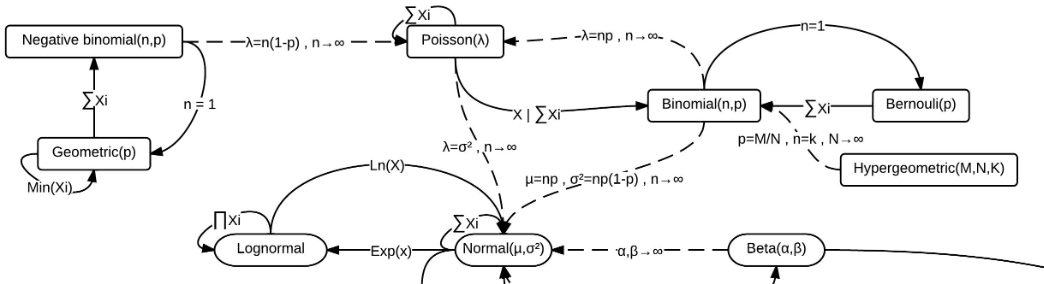
\includegraphics[width=0.7\textwidth]{figs/probs-rel.png}
        \caption{Relationships among some of univariate probability distributions. Source:  \href{https://en.wikipedia.org/wiki/Relationships_among_probability_distributions}{Wikipedia (2019)}}
    \end{figure}
    
    For more see article "Relationships among probability distributions" at \href{https://en.wikipedia.org/wiki/Relationships_among_probability_distributions}{Wikipedia}
\end{frame}

%%%%%%%%%%%% software %%%%%%%%%%%%%%%%%%

\subsection{Practice}

\begin{frame}[fragile]{Overview of main function in open-source packages}
    \begin{table}[]
        \centering
        \caption{Overview of functions}
        \label{tab:my_label}
        \begin{tabular}{c|ccc}
            \hline
            \textbf{Language} & \textbf{R} & \textbf{Python} & \textbf{Julia} \\
            \hline
            Package/module & -- & scipy.stats & Distributions \\
            Density & d<name>() & <name>.pmf() & pdf(<name>)\\
            Cumulative & p<name>() & <name>.cdf() & cdf(<name>) \\
            Quantile & q<name>() & <name>.ppf() & quantile(<name>) \\
            Random & r<name>() & <name>.rvs() & rand(<name>) \\
            \hline
        \end{tabular}
\\
where <name> denotes name of distribution. In R see also \texttt{distributions3} package which mimics \texttt{Distributions.jl} package.
    \end{table}
\end{frame}

\subsection{Exercises}

\begin{frame}{Exercise 1}
    Assume that football player with success rate 0.4 shot 10 times on goal. Let $X$ be a random variable denoting number of successful scores.  Please find:

\begin{enumerate}
    \item Distribution of $X$
    \item Probability that football player score exactly 4 times ($P(X=4)$)
    \item Probability that football player score at least 7 times ($P(X>=7) = 1- P(X <= 6)$)
\end{enumerate}

\end{frame}

\begin{frame}{Exercise 2}
    Number of car accidents in one day in some city follows Poisson distribution with expected value $\lambda=2$. Find the probability that at most 4 car accidents happen.
\end{frame}

\begin{frame}{Exercise 3}
    Read in \texttt{polish-jvs.csv} dataset (Polish Job Vacancy Survey) and do the following:
\begin{enumerate}
    \item Calculate $\hat{\lambda}$ (average number of vacancies). Using the Poisson distribution, calculate $P(X=0)$ and compare with the observed proportion of zeros.
    \item Create a binary variable \texttt{has\_vacancy} ($1$ if vacancies $> 0$, $0$ otherwise). Estimate $\hat{p}$. Using $\mathrm{B}(10, \hat{p})$, calculate $P(Y \geq 3)$.
    \item Generate 1000 random draws from $\mathrm{Pois}(\hat{\lambda})$. Compare with the observed distribution of vacancies.
\end{enumerate}
\end{frame}

\begin{frame}{Interesting discrete distributions}
\begin{itemize}
    \item Beta-Binomial
    \item Zero-inflated Poisson/NB -- when data has more zeros than a standard count distribution predicts; models the data as a mixture of a point mass at zero and a count distribution (Poisson or NB)
    \item Tweedie
    \item Generalized Poisson
\end{itemize}
\end{frame}

\section{Fitting distributions}

\begin{frame}{}
\begin{center}
    \Large{Fitting distributions}
\end{center}    
\end{frame}

\subsection{Maximum likelihood}

\begin{frame}{Maximum likelihood -- theory}
    \begin{itemize}
        \item Maximum likelihood estimation (MLE) is a method of estimating the parameters of a statistical model, given observations.
        \item The method obtains the parameter estimates by finding the parameter values that maximize the likelihood function. 
        \item The estimates are called maximum likelihood estimates, which is also abbreviated as MLE.
        
    \end{itemize}
\end{frame}

\begin{frame}{Maximum likelihood -- theory}
\begin{itemize}
    \item If $f_{i}\left(x_{i} ; \boldsymbol{\theta}\right)$ is the PMF/PDF of a random variable where  $\boldsymbol{\theta}$ is a vector of parameters (e.g. $\lambda$ in Poisson distribution), then for a collection of $N$ independent samples from this distribution, the joint distribution of the random vector $x_i$ is
    \begin{equation}
        L(\boldsymbol{\theta}; \mathbf{x})=\prod_{i=1}^{N} f_{i}\left(x_{i}; \boldsymbol{\theta} \right)
    \end{equation}
\item The maximum likelihood estimate of the parameters  $\boldsymbol{\theta}$ are the parameters which maximize this function with $\boldsymbol{x}$ fixed and given by the data:

\begin{equation}
    \hat{\boldsymbol{\theta}} =\arg \max _{\boldsymbol{\theta}} L(\boldsymbol{\theta}; \mathbf{x} ) =\arg \max _{\boldsymbol{\theta}} l(\boldsymbol{\theta}; \mathbf{x}),
\end{equation}
where the log-likelihood is
\begin{equation}
    l(\boldsymbol{\theta}; \mathbf{x}) = \sum_{i=1}^{N} \log f\left(x_{i}; \boldsymbol{\theta} \right)
\end{equation}
Note: in practice, many optimizers minimize, so we minimize $-l(\boldsymbol{\theta}; \mathbf{x})$.
\end{itemize}
    
\end{frame}

\begin{frame}{Maximum likelihood -- example (Poisson distribution)}

\begin{itemize}
    \item Likelihood function for Poisson distribution is
    \begin{equation}
        L\left(\lambda ; x_{1}, \ldots, x_{n}\right)=\prod_{j=1}^{n} \exp (-\lambda) \frac{1}{x_{j} !} \lambda^{x_{j}}
    \end{equation}
    \item The log-likelihood function is
    \begin{equation}
        l\left(\lambda ; x_{1}, \ldots, x_{n}\right)=-n \lambda-\sum_{j=1}^{n} \ln \left(x_{j} !\right)+\ln (\lambda) \sum_{j=1}^{n} x_{j}
        \end{equation}
    \item The maximum likelihood estimator of $\lambda$
    \begin{equation}
        \hat{\lambda}=\frac{1}{n} \sum_{j=1}^{n} x_{j}
    \end{equation}
\end{itemize}
\end{frame}

\begin{frame}{Score function and Fisher information}
\begin{itemize}
    \item The \textbf{score function} is the gradient of the log-likelihood with respect to $\boldsymbol{\theta}$:
    \begin{equation}
        S(\boldsymbol{\theta}) = \frac{\partial l(\boldsymbol{\theta}; \mathbf{x})}{\partial \boldsymbol{\theta}}
    \end{equation}
    At the MLE, $S(\hat{\boldsymbol{\theta}}) = \boldsymbol{0}$ (first-order condition).
    \item The \textbf{Fisher information} measures the curvature of the log-likelihood:
    \begin{equation}
        I(\boldsymbol{\theta}) = -E\left[\frac{\partial^2 l(\boldsymbol{\theta}; \mathbf{x})}{\partial \boldsymbol{\theta} \partial \boldsymbol{\theta}^T}\right]
    \end{equation}
    \item The observed Fisher information is $\hat{I}(\hat{\boldsymbol{\theta}}) = -H(\hat{\boldsymbol{\theta}})$, where $H$ is the Hessian.
    \item The standard error of the MLE is obtained from:
    \begin{equation}
        \text{SE}(\hat{\theta}_j) = \sqrt{\left[I(\hat{\boldsymbol{\theta}})^{-1}\right]_{jj}} \approx \sqrt{\left[-H(\hat{\boldsymbol{\theta}})^{-1}\right]_{jj}}
    \end{equation}
\end{itemize}
\end{frame}

\begin{frame}{Maximum likelihood -- practice}
\begin{itemize}
    \item Depending on the distribution it is possible to derive closed form for the parameters $\boldsymbol{\theta}$.
    \item In other cases, numerical methods that require gradient (first derivatives) and hessian (second derivatives) are used, for example Newton-Raphson's method:
    \item Statistical packages also implement derivative-free optimization methods that do not require to calculate gradient and hessian.
\end{itemize}
\end{frame}

\begin{frame}{Maximum likelihood -- practice}
    \begin{table}[]
        \centering
        \caption{Overview of functions for ML}
        %\label{tab:my_label}
        \begin{tabular}{cp{3cm}cp{3cm}}
        \hline
          \textbf{Language}   & \textbf{R} &  \textbf{Python} & \textbf{Julia} \\
        \hline
         Packages  & stats, maxLik, optimParallel& scipy.optimize &  Optim, JuMP \\
        Functions & optim(), maxLik(), optimParallel() & minimize() & Optim::optimize(), JuMP::optimize()\\
        \hline
        \end{tabular}
 
    \end{table}
\end{frame}

\begin{frame}{Newton's method -- single parameter function}
    Let $f$: $\mathbb{R}^1 \to \mathbb{R}^1 $ be a differentiable function. We seek a solution of $f'(\theta)=0$, starting from an initial estimate $\theta_0=\theta_1$. 
    
    \vspace{0.5cm}
    
    At the $n$'s step, given $\theta_n$,  compute the next approximation $\theta_{n+1}$ by
    
    \begin{equation}
        \theta_{n+1} = \theta_{n} - \frac{f'(\theta_n)}{f''(\theta_n)}
    \end{equation} 
    
    and repeat until converge (i.e. $|\theta_{n+1}-\theta_n| < \epsilon$).
    
    \vspace{0.5cm}
    
    For step by step examples see: \url{http://amsi.org.au/ESA_Senior_Years/SeniorTopic3/3j/3j_2content_2.html}.
\end{frame}

\begin{frame}{Newton-Raphson algorithm -- multivariate case}
    Newton's method for optimization consists of applying Newton's method for solving systems of equations, where the equations are the first order conditions, saying that the gradient should equal the zero vector.
    
    \begin{equation}
        \nabla \boldsymbol{f}(\boldsymbol{\theta}) = \boldsymbol{0}
    \end{equation}
    
    A second order Taylor expansion of the left-hand side leads to the iterative scheme

\begin{equation}
    \boldsymbol{\theta}_{n+1} = \boldsymbol{\theta}_{n} - \boldsymbol{H}(\boldsymbol{\theta}_n)^{-1}\nabla \boldsymbol{f}(\boldsymbol{\theta}_n),
\end{equation}

where $\nabla \boldsymbol{f}$ is a gradient and $\boldsymbol{H}$ is a hessian of $\boldsymbol{f}$ (second order derivatives). 

\end{frame}

\begin{frame}{Optimization procedures}
    There are plenty of different optimisation procedures that may be used for estimating parameters:
    
    \begin{enumerate}
        \item Gradient free
        \begin{itemize}
            \item Nelder-Mead
            \item Simulated Annealing
            \item Particle Swarm
        \end{itemize}
        \item Gradient required
        \begin{itemize}
            \item Conjugate Gradient Descent
            \item Gradient Descent
            \item (L-)BFGS
        \end{itemize}
        \item Hessian required
            \begin{itemize}
                \item Newton's Method
                \item Newton's Method With a Trust Region
            \end{itemize}
    \end{enumerate}
    
    For more, see \textbf{Optim.jl} documentation \url{https://julianlsolvers.github.io/Optim.jl} or \textbf{scipy.optimize} \url{https://docs.scipy.org/doc/scipy/reference/tutorial/optimize.html}.
\end{frame}

\begin{frame}{Procedures -- fitting specific distributions}
    \begin{table}[]
        \centering
        \caption{Overview of functions}
        %\label{tab:my_label}
        \begin{tabular}{cp{3cm}p{2cm}p{2cm}}
        \hline
          \textbf{Language}   & \textbf{R} &  \textbf{Python} & \textbf{Julia} \\
        \hline
         Packages  & 
         MASS, fitdistrplus, vcd & scipy.stats&  Distributions.jl\\
        Functions &
          MASS::fitdistr(), vcd::goodfit(), fitdistrplus::fitdist() & only continuous distributions & fit(), fit\_mle()\\
        \hline
        \end{tabular}
 
    \end{table}
\end{frame}


\begin{frame}{Practice -- zero-truncated distribution}

\begin{itemize}
    \item Assume that $X$ follows zero-truncated Poisson distribution given by 
    
    \begin{equation}
        P(X=x, X>0; \lambda) = \frac{f(x; \lambda)}{1 - f(0;\lambda)} = \frac{\lambda^x e^{-\lambda}}{x!(1-e^{-\lambda})} =  \frac{\lambda^x}{(e^\lambda-1)x!},
        \label{eq-ztpoisson}
    \end{equation}
    complete the following task:
    
    \item estimate $\lambda$ based on the maximum likelihood estimation method.
    \item Note that, obtaining $\lambda$ requires deriving log-likelihood function (also gradient with respect to $\lambda$) and applying optimization procedure (e.g. \texttt{optim} function).
\end{itemize}

\end{frame}

\begin{frame}{Zero-truncated distributions -- capture-recapture}
\begin{itemize}
    \justifying
    \item Zero-truncated distributions are used to model the size of hard-to-reach populations, for instance: homeless, civilian casualties in wars, irregular population or drunk drivers.
    \item Methods to estimate the size of the population are called \textbf{capture-recapture methods}. We will discuss them further in the lecture.
    \item The main assumption is as follows: the true generating process is following Poisson distribution but data was truncated i.e. we observe only positive counts (1, 2, 3, 4...). Note that this is for a simple, naive model without covariates.
    \item These counts refer to number of re-capures: 1 - captured only once, 2 - captured twice, 3 - capture three times etc. Example, following van der Heijden et al. (2003):
    \begin{table}
        \centering
        \caption{Dutch irregular immigrants in 1995 (not effectively expelled)}
        \begin{tabular}{r|rrrrrrr|r}
        \hline
        N    &  $0$ & $1$ & $2$ & $3$ & $4$  & $5$ & $6$ & $n$\\
        \hline
        unknown    &  unknown  & 1645 & 183 & 37 & 13 & 1 & 1 & 1880\\
         \hline     
        \end{tabular}
    \end{table}
\end{itemize}
\end{frame}


\begin{frame}{Zero-truncated distributions -- capture-recapture}
To estimate the size of the population of irregular immigrants assuming the Poisson distribution we need to follow the steps:
\begin{enumerate}
    \item estimate unknown $\lambda$ parameter assuming zero-truncated Poisson distribution given \eqref{eq-ztpoisson}
    \item estimate the population size using the following estimator
    \begin{equation}
        \hat{N} = \frac{n}{1 - f(x = 0; \hat{\lambda})},
    \end{equation}
    where $n$ is the observed number of counts and $f$ is the pdf of Poisson.
    \item estimate the variance of this estimator (omitted here).
\end{enumerate}
\end{frame}

\begin{frame}[allowframebreaks, fragile]{Practice -- exercise \#1 -- solution}
We start with likelihood function

\begin{equation}
    L = \prod_i \frac{\lambda^x_i}{(e^\lambda-1)x_i!},
\end{equation}

then we compute log-likelihood

\begin{equation}
    l(\lambda; \mathbf{x}) = \log
    \left(
    \prod_i \frac{\lambda^x_i}{(e^\lambda-1)x_i!}
    \right) = 
    \sum_i \log 
    \left( 
    \frac{\lambda^x_i}{(e^\lambda-1)x_i!}
    \right)
\end{equation}
after simplification we get

\begin{equation}
   l(\lambda; \mathbf{x}) = \sum_i x_i \log \lambda - \sum_i \log(e^\lambda-1) - \sum_i \log(x_i!) 
\end{equation}

\newpage

In order to get estimate of $\lambda$ we need to calculate derivatives with respect to this parameter. Thus, gradient is given by 

\begin{equation}
    \frac{\partial l}{\partial \lambda} = \frac{\sum_i x_i}{\lambda} - \frac{n e^\lambda}{e^\lambda - 1} = 
    \frac{\sum_i x_i}{\lambda} - n \frac{e^\lambda}{e^\lambda - 1}.    
\end{equation}

We can also calculate second derivative (hessian)

\begin{equation}
    \frac{\partial^2 l}{\partial \lambda^2} =  - \frac{\sum_i x_i}{\lambda^2} + n \frac{e^\lambda}{(e^\lambda-1)^2}.
\end{equation}

Based on that we can apply Newton-Raphson method. Here's possible solution using R, \texttt{maxLik} and  \texttt{extraDistr}.

\begin{verbatim}
library(maxLik)
library(extraDistr) ## rtpois

## log-likelihood function
ll <- function(par, x) {
  m <- sum(x)*log(par)-length(x)*log(exp(par)-1)
  m
}

## gradient
grad <- function(par, x)  {
  g <- sum(x) / par - length(x)*exp(par)/(exp(par)-1)
  g
}


## hessian
hess <- function(par, x) {
  h <- -sum(x)/par^2 + length(x)*exp(par)/(exp(par)-1)^2 
  h
}

d <-  c(1645,183,37, 13,1,1)
x <- rep(1:6,d)
## without gradient and hessian
res <- maxLik(logLik = ll, start = 1, x = x, method = "NR")

## with gradient and hessian
res2 <- maxLik(logLik = ll,  grad = grad, 
            hess = hess, start = 1, x = x, method = "NR")
\end{verbatim}

\newpage

Results for the approach without specifying gradient and hessian (they are calcuated using numerical methods, see \texttt{numDeriv} package).
\begin{verbatim}
--------------------------------------------
Maximum Likelihood estimation
Newton-Raphson maximisation, 6 iterations
Return code 8: successive function values within 
relative tolerance limit (reltol)
Log-Likelihood: -656.1294
1  free parameters
Estimates:
     Estimate Std. error t value Pr(> t)
[1,]  0.30862    0.01725   17.89  <2e-16 ***
---
Signif. codes:  0 ‘***’ 0.001 ‘**’ 0.01 ‘*’ 0.05 ‘.’ 0.1 ‘ ’ 1
--------------------------------------------
\end{verbatim}

\newpage

Results for approach with specifying gradient and hessian.
\begin{verbatim}
--------------------------------------------
Maximum Likelihood estimation
Newton-Raphson maximisation, 6 iterations
Return code 8: successive function values within 
relative tolerance limit (reltol)
Log-Likelihood: -656.1294
1  free parameters
Estimates:
     Estimate Std. error t value Pr(> t)
[1,]  0.30862    0.01726   17.88  <2e-16 ***
---
Signif. codes:  0 ‘***’ 0.001 ‘**’ 0.01 ‘*’ 0.05 ‘.’ 0.1 ‘ ’ 1
--------------------------------------------
\end{verbatim}
\end{frame}



\begin{frame}[fragile]{Practice - exercise \#1 -- by hand}
    \begin{verbatim}
x_0 <- 0.5 ## starting point

for (i in 1:10) { 
  
  x_1 <- x_0 - grad(x_0, x)/hess(x_0, x)
  
  if ( abs(x_0 - x_1) < 0.001) {
    cat("Result:", x_1, "\n")
    cat("Algorithm converged after: ", i, " iterations.")
    break()
    
  }
  x_0 <- x_1

}
\end{verbatim}
\end{frame}

\begin{frame}[fragile]{Practice - exercise \#1 -- using pdf}
    \begin{verbatim}
ll <- function(x, par) {
  m <- dtpois(x, lambda = par, a = 0, log = TRUE)
  sum(m)
}

d <-  c(1645,183,37, 13,1,1)
x <- rep(1:6,d)
res <- maxLik(logLik = ll, start = 1, x = x, method = "NR")
summary(res)
    \end{verbatim}
\end{frame}

\begin{frame}[fragile]{Practice - exercise \#1 -- optim}

Optim is a MINIMIZATION procedure and for scalars Brent's method is used. 

    \begin{verbatim}

ll <- function(par, x) {
  m <- sum(x)*log(par)-length(x)*log(exp(par)-1)
  -sum(m)
}

## gradient
grad <- function(par, x)  {
  g <- sum(x) / par - length(x)*exp(par)/(exp(par)-1)
  -sum(g)
}

optim(par = 0.5, fn = ll, gr = grad, 
      method = "Brent", lower = 0, upper = 10, x = x, 
      hessian = TRUE)
\end{verbatim}
\end{frame}




\begin{frame}[fragile]{Practice - exercise \#1 -- numDeriv}
Numerical Differentiation (see \url{https://github.com/bob-carpenter/ad-handbook/blob/master/ad-handbook-draft.pdf})

\begin{verbatim}
library(numDeriv)
ll_func <- function(y, par) {
     m <- sum(y)*log(par)-length(y)*log(exp(par)-1)
     -sum(m)
}
grad_func <- function(y, par)  {
     g <- sum(y) / par - length(y)*exp(par)/(exp(par)-1)
     -sum(g)
}
numDeriv::grad(ll, x = 0.3086189, y = x)
[1] -0.0001720925
grad_func(y = x, par = 0.3086189)
[1] -1.147304e-05
\end{verbatim}
\end{frame}


\subsection{Assessment of the fit}

\begin{frame}{Fitting discrete distributions}

Fitting a discrete distribution involves three basic steps:

    \begin{enumerate}
    \justifying
        \item Estimating the parameter(s) of the distribution from the data -- typically using maximum likelihood;
        \item From this, we can calculate the fitted probabilities ($\hat{p}_k$) or equivalently, the model expected frequencies ($\hat{p}_k n$) [based on the CDF];
        \item Finally, we can calculate goodness-of-fit test measuring the departure between the observed and fitted frequencies;
    \end{enumerate}

 \begin{itemize}
    \item If we would like to compare two different distributions on a given data we may use information criteria (e.g. AIC or BIC);
    \item Moreover, the selection of a distribution should also be driven by knowledge of underlying processes when available.
 \end{itemize}
\end{frame}

\begin{frame}{Assessment of the fit -- tests}

Often goodness-of-fit is examined with a classical (Pearson) goodness-of-fit (GOF) chisquare test
    
    \begin{equation}
        \chi^2 = \sum_{k=1}^{K} \frac{\left(n_{k}-n \hat{p}_{k}\right)^{2}}{n \hat{p}_{k}} \sim \chi^{2}(K-s-1),
    \end{equation}
    
    where $n_k$ is the observed frequency for category $k$, $\hat{p}_k$ is the fitted probability, $K$ is the number of categories, and $s$ is the number of estimated parameters. An alternative test statistic is the likelihood-ratio $G^2$ statistic
    
    \begin{equation}
        G^{2}=2\sum_{k=1}^{K} n_{k} \log \left(\frac{n_{k}}{n \hat{p}_{k}}\right) \sim \chi^2(K-s-1).
    \end{equation}
\end{frame}

\begin{frame}{Assessment of the fit -- assumptions}
    The $\chi^2$ and $G^2$ tests rely on a large-sample approximation. The approximation is reliable when:
    \begin{itemize}
        \item Most expected frequencies satisfy $n\hat{p}_k \geq 5$;
        \item No expected frequency is below 1;
        \item The total sample size $n$ is sufficiently large.
    \end{itemize}

    \vspace{0.3cm}
    When these conditions are violated (sparse data, many categories with low counts):
    \begin{itemize}
        \item Merge adjacent low-frequency categories until the condition is met;
        \item Use a parametric bootstrap to obtain the p-value empirically;
        \item The \texttt{vcd::goodfit()} warning \textit{``Chi-squared approximation may be incorrect''} is triggered when any $n\hat{p}_k < 5$.
    \end{itemize}
\end{frame}

\begin{frame}{Information Criteria}
    \begin{itemize}
        \item AIC
        $$
        \text{AIC} = 2s - 2\log(\hat{L}),
        $$
        \item BIC
        $$
        \text{BIC} = \log(n) \cdot s - 2\log(\hat{L}),
        $$
         where $s$ is the number of parameters, $n$ is the number observations and $\log(\hat{L})$ is the value log-likelihood function estimated for a given distribution.
         \item To compare two distributions on the same data we may use a likelihood ratio test given by:
         $$
         \text{LR} = -2\log\left(\frac{\hat{L}_1}{\hat{L}_2}\right) = 2\log(\hat{L}_2) - 2\log(\hat{L}_1) \sim \chi^2(s_2-s_1),
         $$
         where $\hat{L}_1$ is the likelihood of the first (simpler) distribution and $\hat{L}_2$ of the second, $s_1$ and $s_2$ denote the number of parameters of the first and second distribution.
    \end{itemize}


\end{frame}

\begin{frame}{Nested vs non-nested models}
    The LR test requires \textbf{nested models}: model $M_1$ is nested in $M_2$ if $M_1$ is a special case of $M_2$ obtained by fixing some parameters.

    \vspace{0.3cm}
    \textbf{Examples of nested pairs:}
    \begin{itemize}
        \item Poisson ($s=1$) $\subset$ Negative Binomial ($s=2$): set $\theta \to \infty$ in NB $\Rightarrow$ Poisson;
        \item Binomial ($s=1$, fixed $n$) $\subset$ Beta-Binomial ($s=2$, fixed $n$).
    \end{itemize}

    \vspace{0.3cm}
    \textbf{Non-nested examples} (LR test does not apply):
    \begin{itemize}
        \item Poisson vs Geometric -- neither is a special case of the other;
        \item ZIP vs Hurdle -- different structural assumptions about zeros.
    \end{itemize}

    \vspace{0.3cm}
    \begin{table}[]
        \centering
        \small
        \begin{tabular}{lll}
        \hline
        \textbf{Tool} & \textbf{Purpose} & \textbf{Requirement} \\
        \hline
        $\chi^2$ / $G^2$ & Does \textit{one} model fit the data? & Single model \\
        AIC / BIC & Which model fits \textit{better}? & $\geq 2$ models (any) \\
        LR test & Is the improvement \textit{significant}? & Nested models \\
        \hline
        \end{tabular}
    \end{table}
\end{frame}

\begin{frame}{Visual inspection}
\begin{itemize}
    \item A fitted distribution should be evaluated using graphical methods.
    \item There are plenty of ways to verify whether the distribution fits given data. One way to assess it is to use \textbf{rootogram}.
    \item John Tukey introduced the Hanging Rootogram in 1971, for more details see Kleiber \& Zeileis (2016). Visualizing count data regressions using rootograms. The American Statistician, 70(3), 296-303.
\end{itemize}
\end{frame}

\begin{frame}{Exploratory Data Analysis}
    \begin{figure}
        \centering
        
\includegraphics[width=0.7\textwidth]{figs/tukey.jpg}
    \end{figure}
\end{frame}


\begin{frame}{Rootogram}
    \begin{figure}
        \centering
        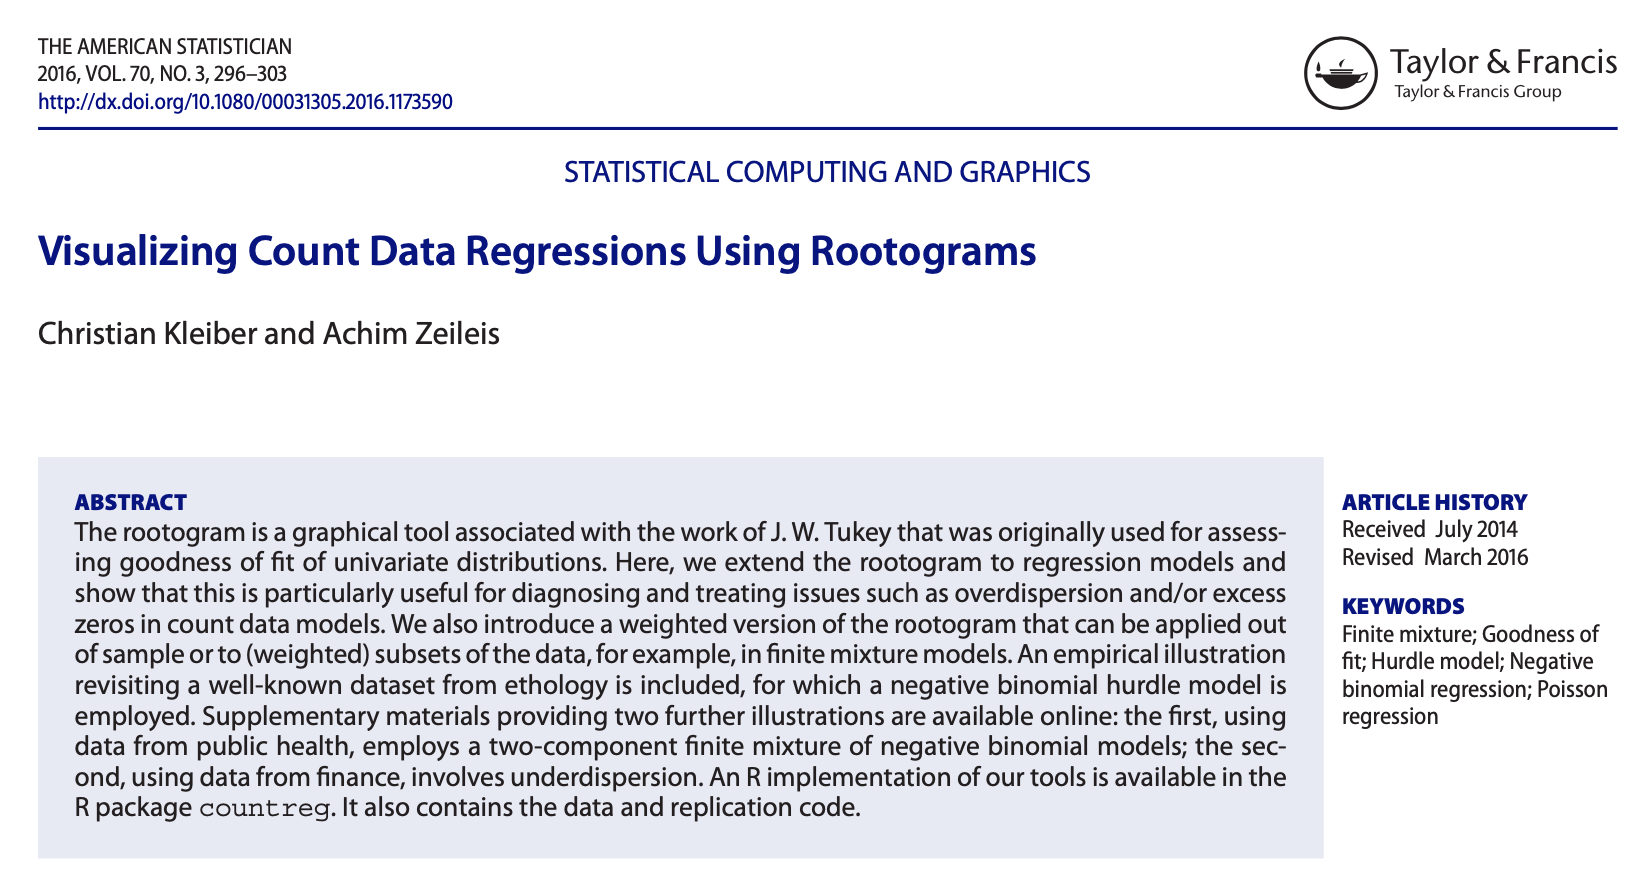
\includegraphics[width=0.7\textwidth]{figs/rootogram0.png}
    \end{figure}
\end{frame}

\begin{frame}{Rootogram}
    \begin{figure}
        \centering
        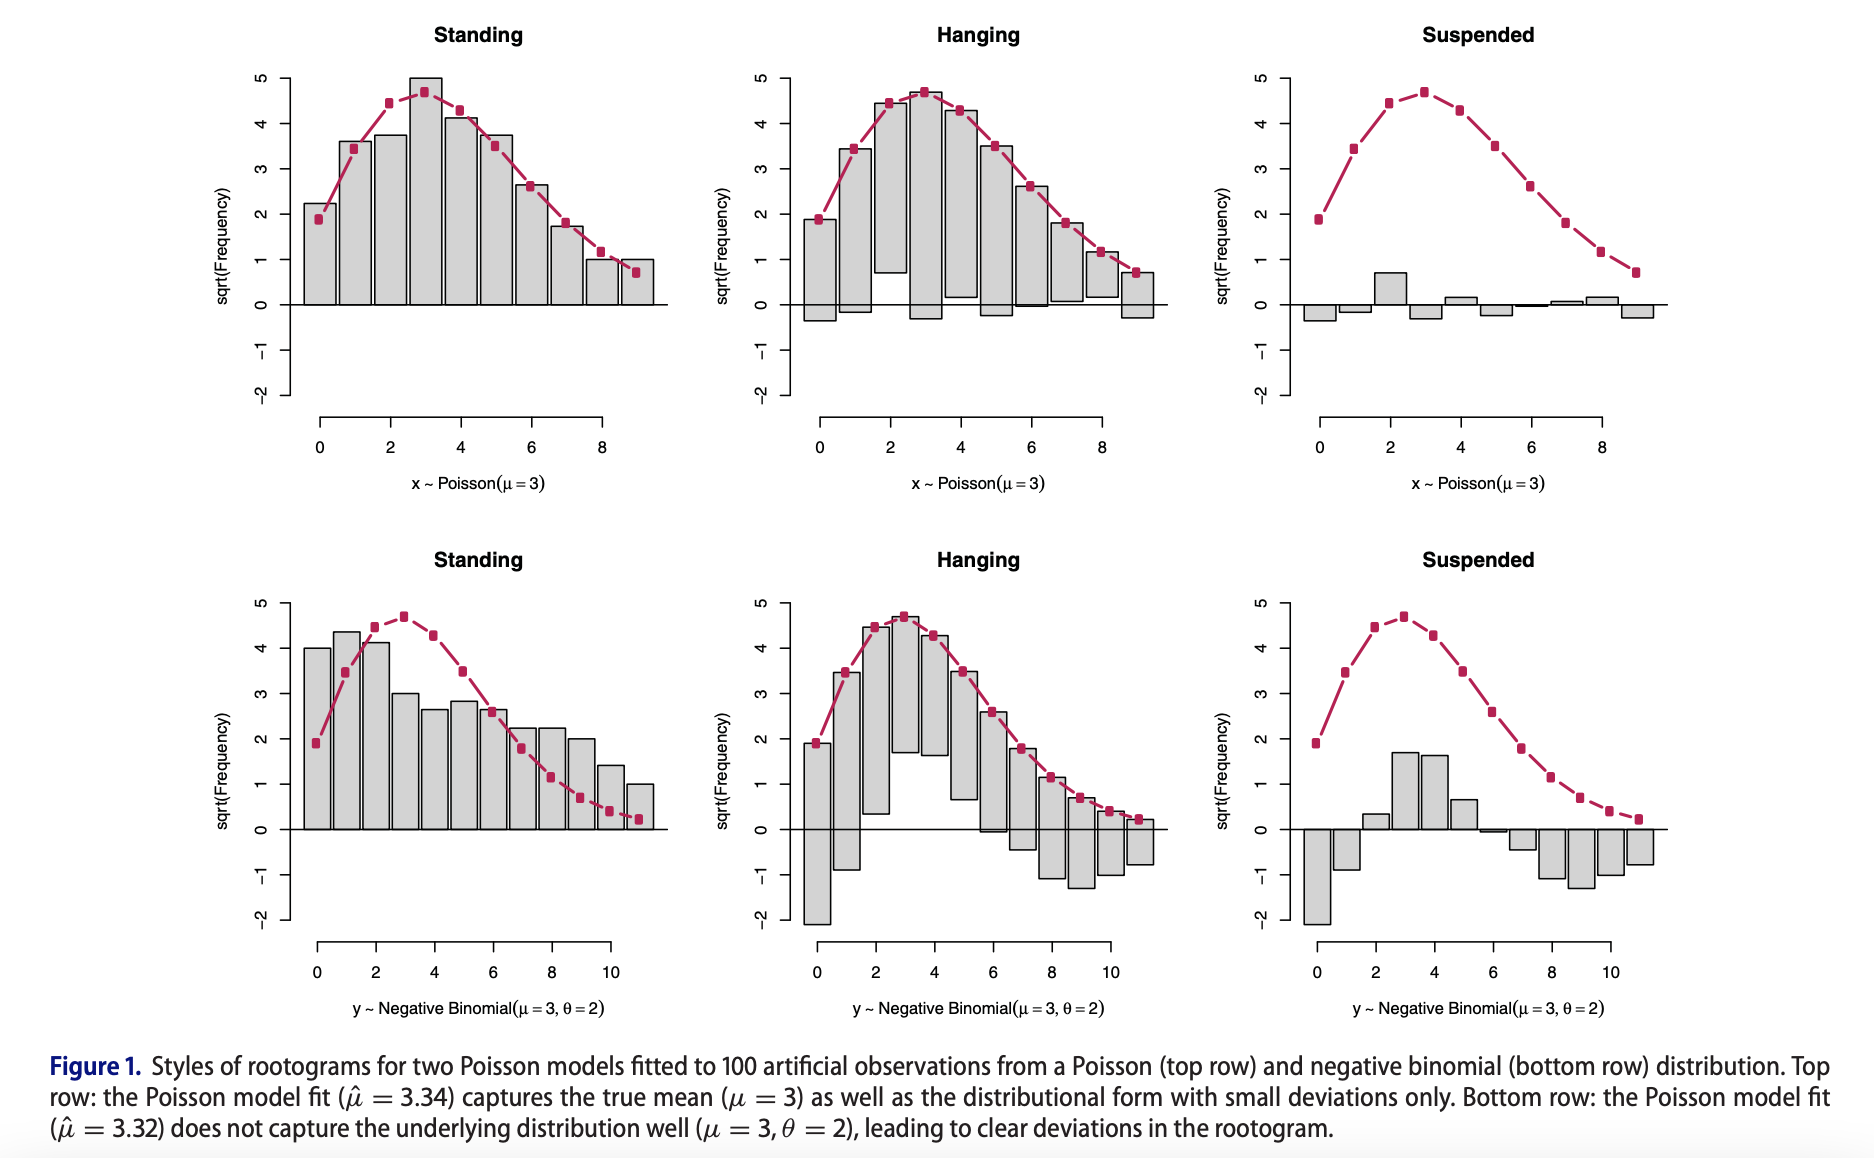
\includegraphics[width=0.7\textwidth]{figs/rootogram1.png}
        \caption{Source: Kleiber \& Zeileis (2016)}
    \end{figure}
\end{frame}

\begin{frame}{Rootogram}
    \begin{figure}
        \centering
        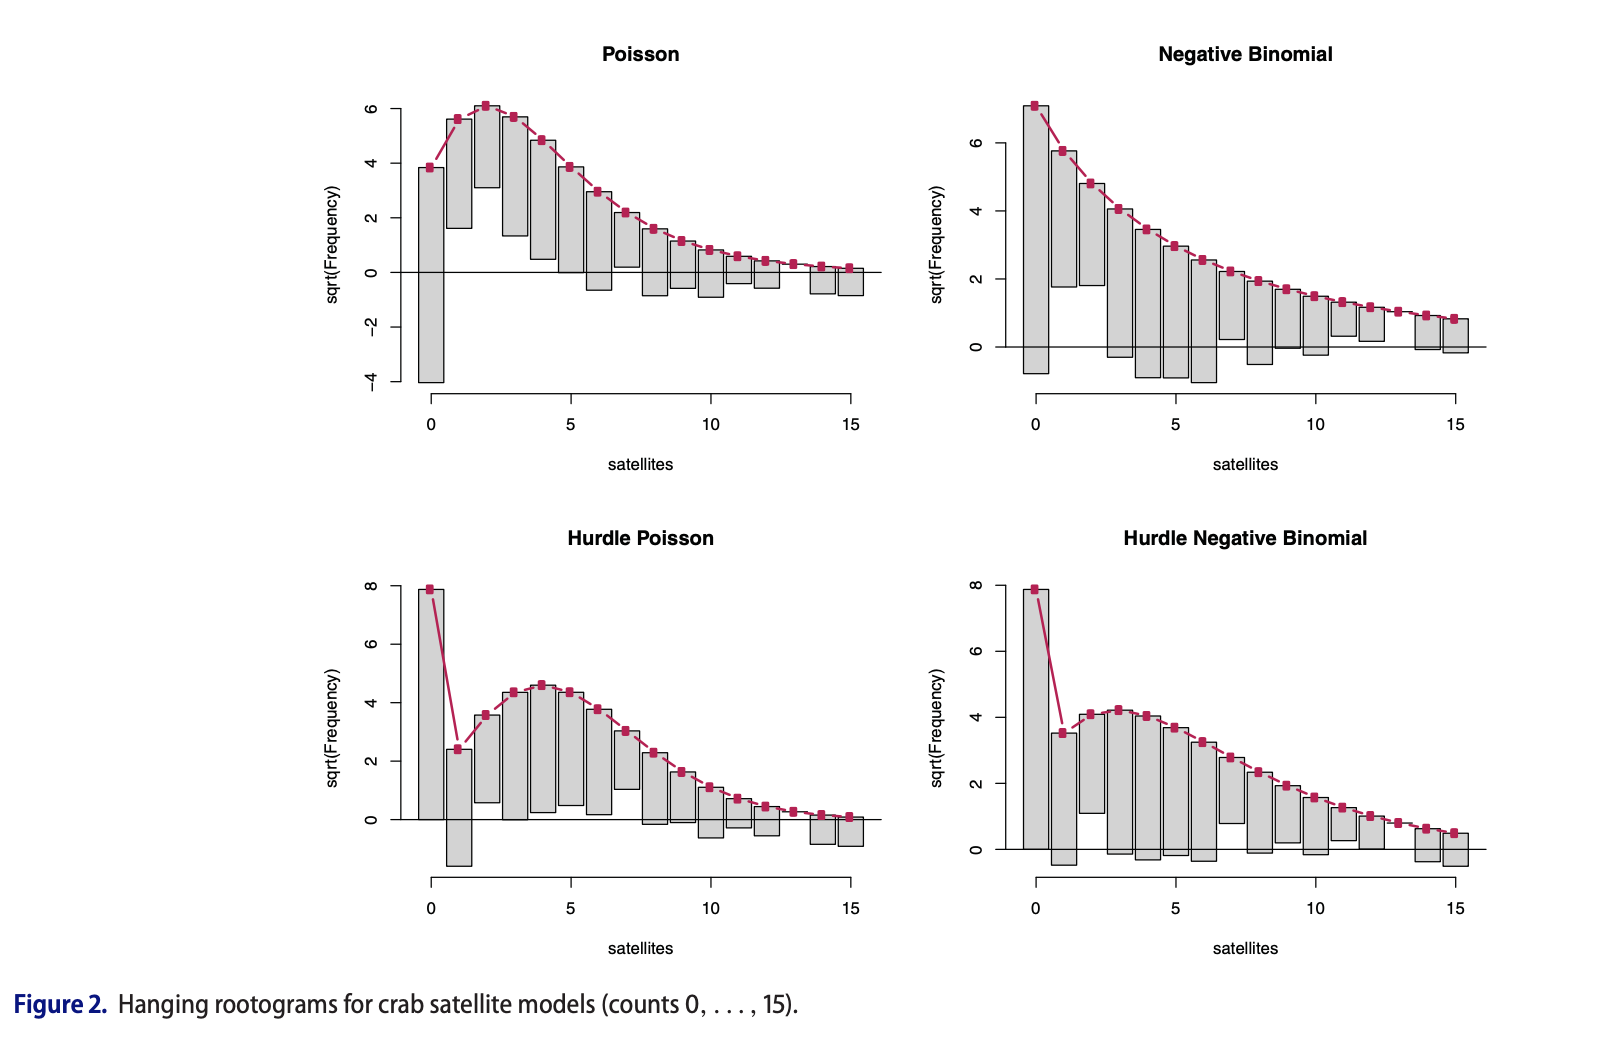
\includegraphics[width=0.7\textwidth]{figs/rootogram2.png}
        \caption{Source: Kleiber \& Zeileis (2016)}
    \end{figure}
\end{frame}

\begin{frame}{Rootogram -- interpretation}
    In a \textbf{hanging rootogram} (Tukey, 1971; Kleiber \& Zeileis, 2016):
    \begin{itemize}
        \item The \textbf{red curve} shows fitted (expected) frequencies on the square-root scale: $\sqrt{n\hat{p}_k}$;
        \item The \textbf{bars hang down} from the curve so their bottom edges indicate the deviation;
        \item The \textbf{reference line is at 0} -- bars ending \textit{below} 0 indicate the model \textit{overpredicts} that count; bars ending \textit{above} 0 indicate the model \textit{underpredicts};
        \item A good fit: all bar bottoms are close to the zero line.
    \end{itemize}

    \vspace{0.3cm}
    Why square root? It stabilizes the variance of Poisson-like counts, making deviations visually comparable across different frequency levels.
\end{frame}

\begin{frame}{Procedures -- fitting specific distributions}
    \begin{table}[]
        \centering
        \caption{Overview of functions}
        %\label{tab:my_label}
        \begin{tabular}{cp{3.5cm}p{2.5cm}p{2.5cm}}
        \hline
          \textbf{Task}   & \textbf{R} &  \textbf{Python} & \textbf{Julia} \\
        \hline
         Fitting  &
         MASS::fitdistr(), fitdistrplus::fitdist() & scipy.stats.fit() &  Distributions.jl, fit() \\
         GoF test &
          chisq.test(), vcd::goodfit() & scipy.stats.chisquare(ddof=s) & HypothesisTests.jl, ChisqTest()\\
         Rootogram &
          vcd::rootogram(), countreg::rootogram() & -- & -- \\
        \hline
        \end{tabular}
    \end{table}
\end{frame}

\begin{frame}[fragile]{Example} 
Install required packages
\begin{verbatim}
install.packages("vcd")
install.packages("fitdistrplus")
install.packages("countreg", 
                 repos="http://R-Forge.R-project.org")
\end{verbatim}
\end{frame}

\begin{frame}[fragile]{Example}
Generate two vectors $y \sim NB(\mu=3,\theta=2)$ and $x \sim Po(3)$

\begin{verbatim}
set.seed(1)
n <- 500
y <- rnbinom(n, mu = 3, size = 2)
x <- rpois(n, lambda = 3)
\end{verbatim}
\end{frame}

\begin{frame}[fragile]{Example (MASS and fitdistrplus)}
\small
\begin{itemize}
    \item Using \texttt{MASS} package 
    \begin{verbatim}
> fitdistr(x = y, densfun = "negative binomial")

     size         mu    
  2.0890650   2.7621469 
 (0.2513296) (0.1132676)
    \end{verbatim}
    \item Using \texttt{fitdistrplus} package
    \begin{verbatim}
> summary(fitdist(data = y, method = "mle", distr = "nbinom"))
Fitting of the distribution ' nbinom ' by maximum likelihood 
Parameters : 
     estimate Std. Error
size 2.089736  0.2514846
mu   2.761956  0.1132449

Loglikelihood:  -1066.958   AIC:  2137.916   BIC:  2146.345 
      
    \end{verbatim}
\end{itemize}
\end{frame}

\begin{frame}[fragile]{Example (vcd)}
\small
\begin{verbatim}
> goodfit(y, "nbinomial")

Observed and fitted values for nbinomial distribution
with parameters estimated by `ML' 

 count observed      fitted pearson residual
     0       86  86.0170786     -0.001841454
     1      100 102.3135531     -0.228724611
     2       91  89.9760131      0.107952084
     3       77  69.8274259      0.858345287
     4       46  50.5825323     -0.644325401
     5       36  35.0733866      0.156462307
     6       22  23.5945631     -0.328273428
     7       11  15.5241830     -1.148248236
     8       13  10.0423304      0.933323943
     9        6   6.4097257     -0.161835389
    10        4   4.0469786     -0.023352549
    11        5   2.5323718      1.550657921
    12        1   1.5727199     -0.456684796
    13        1   0.9704803      0.029965307
    14        0   0.5955491     -0.771718251
    15        0   0.3637086     -0.603082616
    16        0   0.2211813     -0.470299194
    17        1   0.1340023      1.144759231
\end{verbatim}
\end{frame}

\begin{frame}[fragile]{Example (vcd)}
    \begin{itemize}
        \item Goodness of fit statistic
\begin{verbatim}
> summary(goodfit(y, "nbinomial"))

Goodness-of-fit test for nbinomial distribution

                      X^2 df  P(> X^2)
Likelihood Ratio 10.79421 12 0.5466328
\end{verbatim}
        \item Rootogram
\begin{verbatim}
plot(goodfit(y, "nbinomial"))
\end{verbatim}
    \end{itemize}

\vspace{0.2cm}
\alert{Note:} \texttt{goodfit()} with \texttt{method="ML"} uses $\text{df} = K^{*} - 1 - s$ where $K^{*}$ is the number of categories with \textit{non-zero} observed counts (here $K^{*} = 15$), giving $\text{df} = 15 - 1 - 2 = 12$. This differs from \texttt{chisq.test()} which uses all $K$ categories.
\end{frame}

\begin{frame}[fragile]{Example (countreg)}
\begin{verbatim}
countreg::rootogram(y, "poisson")
countreg::rootogram(y, "negbin")
\end{verbatim}
\end{frame}

\begin{frame}[fragile, allowframebreaks]{Example -- GoF step by step}
\begin{enumerate}
    \item Fit selected distribution to data
    \begin{verbatim}
est_params <- fitdistr(x = y, densfun = "negative binomial")        
    \end{verbatim}
    \item Calculate cumulative distribution function (CDF)
    \begin{verbatim}
range <- min(y):max(y)
n <- length(range)
est_cdf <- c(0, 
             pnbinom(q = range[-n], 
                     size = est_params$estimate["size"], 
                     mu = est_params$estimate["mu"]),
             1)
    \end{verbatim}
    \item Calculate probabilities (PMF)
    \begin{verbatim}
est_pmf <- diff(est_cdf)
    \end{verbatim}
\item Calculate $\chi^2$ goodness of fit using \texttt{chisq.test} function
\begin{verbatim}
df <- data.frame(y_vals = range)
df_freq <- as.data.frame(table(y))
names(df_freq) <- c("y_vals", "n_obs")
df <- merge(x = df, y = df_freq, by = "y_vals", all.x = T)
df$n_obs[is.na(df$n_obs)] <- 0
df$p_hat <- est_pmf

chisq.test(x = df$n_obs, p = df$p_hat)

	Chi-squared test for given probabilities

data:  df$n_obs
X-squared = 8.6693, df = 17, p-value = 0.9501
\end{verbatim}

\alert{WARNING!} p-value calculated according to this method is incorrect! Why? The \texttt{chisq.test} function does not account for estimated parameters. It uses $\text{df} = K - 1 = 17$, but the correct degrees of freedom are $\text{df} = K - 1 - s = 18 - 1 - 2 = 15$ (NB has $s=2$ parameters).

\item Correct p-value 

\begin{verbatim}
> pchisq(8.6693, df = 15, lower.tail = FALSE)

0.8941643

\end{verbatim}
\end{enumerate}
\end{frame}

\begin{frame}[fragile]{Example -- GoF in Python}
\small
\begin{verbatim}
import numpy as np
import scipy.stats as st

np.random.seed(1)
n = 500
y = st.nbinom.rvs(n=2, p=2/(2+3), size=n)

## fit NB via method of moments
mu_hat = y.mean()
var_hat = y.var(ddof=1)
size_hat = mu_hat**2 / (var_hat - mu_hat)
prob_hat = size_hat / (size_hat + mu_hat)

## expected frequencies
rng = np.arange(y.min(), y.max() + 1)
obs = np.array([(y == k).sum() for k in rng])
pmf = st.nbinom.pmf(rng, n=size_hat, p=prob_hat)
pmf[-1] += 1 - pmf.sum()
exp_f = n * pmf

## WRONG (ddof=0, ignores estimated parameters)
st.chisquare(obs, f_exp=exp_f)
## CORRECT (ddof=2 for NB with s=2 parameters)
st.chisquare(obs, f_exp=exp_f, ddof=2)
\end{verbatim}
\end{frame}

\begin{frame}[fragile]{Example (vcd) -- warning}
    Note that we may specify $\chi^2$ GoF test in \texttt{vcd} package but it gives a different value of $\chi^2$ statistic as parameters are not estimated using ML method.

\begin{verbatim}
> object <- goodfit(y, type = "nbinomial", method = "MinChisq")
> summary(object)

	 Goodness-of-fit test for nbinomial distribution

             X^2 df  P(> X^2)
Pearson 8.082266 15 0.9204422
Warning message:
In summary.goodfit(object) : Chi-squared approximation may be incorrect
\end{verbatim}
\end{frame}

\subsection{Comparison of estimation methods}

\begin{frame}{Comparison of estimation methods}
\small
    \begin{table}[]
        \centering
        \begin{tabular}{p{1.5cm}p{2.5cm}p{2.5cm}p{3.5cm}}
        \hline
        \textbf{Method} & \textbf{Objective} & \textbf{Requirements} & \textbf{When to use} \\
        \hline
        MLE & Maximize $l(\boldsymbol{\theta}; \mathbf{x})$ & Full distributional assumption & Default choice; efficient when model is correctly specified \\[0.3cm]
        GMM & Match sample \& theoretical moments & Only moment conditions $E[g(X;\boldsymbol{\theta})]=0$ & When distribution is unknown but moments are known \\[0.3cm]
        EM & Maximize $l(\boldsymbol{\theta})$ iteratively via $Q(\boldsymbol{\theta}|\boldsymbol{\theta}^{(t)})$ & Complete-data likelihood + latent structure & Missing data, mixtures, zero-truncated/ inflated models \\[0.3cm]
        Profile L. & Maximize $l_P(\psi) = \max_{\boldsymbol{\nu}} l(\psi, \boldsymbol{\nu})$ & Full distributional assumption & Inference on a subset of parameters; CI via LR \\[0.3cm]
        QMLE & Maximize quasi-log-likelihood & Only mean-variance relationship & Overdispersion; robust to misspecification of higher moments \\
        \hline
        \end{tabular}
    \end{table}
\end{frame}

\subsection{Further reading}

\begin{frame}{Further reading -- MLE extensions}
\begin{itemize}
    \item \textbf{Expectation-Maximization (EM) algorithm} -- iterative method for MLE when data has latent/missing structure (e.g., zero-inflated models, mixture models). Relevant for capture-recapture and incomplete data problems.
    \item \textbf{Profile likelihood} -- useful when dealing with nuisance parameters. Instead of jointly optimizing all parameters, we maximize over nuisance parameters for each fixed value of the parameter of interest.
    \item \textbf{Quasi-likelihood / pseudo-likelihood} -- relaxes full distributional assumptions; requires only specification of the mean-variance relationship. Important bridge to GLMs, especially for overdispersed count data.
\end{itemize}
\end{frame}

\begin{frame}{Further reading -- GoF extensions}
\begin{itemize}
    \item \textbf{Vuong test} -- for comparing non-nested models (e.g., ZIP vs ZINB, Poisson vs Hurdle). Complements the LR test which requires model nesting.
    \item \textbf{Dispersion test} -- formal test for overdispersion (Cameron-Trivedi test). Tests $H_0: \text{Var}(X) = E(X)$ against $H_1: \text{Var}(X) = E(X) + \alpha \cdot g(E(X))$. In R: \texttt{AER::dispersiontest()}.
    \item \textbf{Randomized quantile residuals (PIT)} -- modern alternative to rootograms for assessing distributional fit. Transforms discrete data to continuous uniform under the fitted model. In R: \texttt{DHARMa} package.
\end{itemize}
\end{frame}

\begin{frame}{Further reading -- additional topics}
\begin{itemize}
    \item \textbf{Bootstrap for GoF} -- when asymptotic $\chi^2$ approximation is unreliable (small expected counts, sparse contingency tables). Parametric bootstrap simulates data from the fitted model and computes the GoF statistic distribution empirically.
    \item \textbf{Key references}:
    \begin{itemize}
        \item Agresti, A. (2013). \textit{Categorical Data Analysis}. Wiley.
        \item Kleiber, C. \& Zeileis, A. (2016). Visualizing count data regressions using rootograms. \textit{The American Statistician}, 70(3), 296--303.
        \item Cameron, A.C. \& Trivedi, P.K. (2013). \textit{Regression Analysis of Count Data}. Cambridge University Press.
    \end{itemize}
\end{itemize}
\end{frame}

\section{Linear regression}

\subsection{Categorical variables in regression}

\begin{frame}{Categorical variables in regression -- recap}
Recall: a categorical variable with $k$ levels is represented in a regression
model by $k-1$ indicator (dummy) variables to avoid rank deficiency.

\medskip
\textbf{Example.} Let \texttt{woj} (voivodeship) have $k=16$ levels with
reference \texttt{02}. The regression model is:
\begin{equation}
    \text{vacancies}_i = \beta_0 + \beta_1 I(\text{woj}_i\!=\!\texttt{04})
    + \beta_2 I(\text{woj}_i\!=\!\texttt{06}) + \cdots
    + \beta_{15} I(\text{woj}_i\!=\!\texttt{32}) + \varepsilon_i.
\end{equation}

Each $\beta_j$ represents the \textbf{difference in expected vacancies} between
voivodeship $j$ and the reference voivodeship (\texttt{02}).

\medskip
The intercept $\beta_0$ equals the mean of the reference group.
\end{frame}


\begin{frame}{Why is $\hat{\beta}_0$ the mean of the reference level?}
For an observation in the reference group (\texttt{woj} = \texttt{02}), \emph{all} dummies are 0, so the model collapses to:
\[
E(\text{vacancies} \mid \text{woj} = \texttt{02}) = \beta_0 + \beta_1 \cdot 0 + \cdots + \beta_{15} \cdot 0 = \beta_0.
\]

\medskip
Under OLS, the fitted value for a group equals the \textbf{sample mean} of that group (the mean minimises the squared deviations within the group). Therefore:
\[
\hat{\beta}_0 = \bar{Y}_{\text{ref}}, \qquad \hat{\beta}_j = \bar{Y}_j - \bar{Y}_{\text{ref}}.
\]

\medskip
\textbf{JVS data check:}
\begin{table}[h]\centering\small
\begin{tabular}{lcc}
\hline
& $\bar{Y}_j$ (sample) & Reconstructed from coefficients \\
\hline
\texttt{woj = 02} (ref) & 1.182 & $\hat{\beta}_0 = 1.182$ \\
\texttt{woj = 04}       & 0.569 & $\hat{\beta}_0 + \hat{\beta}_1 = 1.182 - 0.613 = 0.569$ \\
\hline
\end{tabular}
\end{table}

\medskip
\alert{Each $\hat{\beta}_j$ is a difference in sample means.}
\end{frame}


\begin{frame}{What happens when coding is wrong?}
If \texttt{woj} is treated as a \textbf{numeric} variable (02, 04, 06, \ldots, 32),
the model becomes:
\begin{equation}
    \text{vacancies}_i = \beta_0 + \beta_1 \cdot \text{woj}_i + \varepsilon_i.
\end{equation}

This assumes:
\begin{itemize}
    \item A \textbf{linear} relationship between the code number and vacancies,
    \item \textbf{Equal spacing}: going from 04 to 06 has the same effect as
          going from 28 to 30,
    \item A \textbf{single slope} $\beta_1$ summarises all 16 regions.
\end{itemize}

\medskip
\textbf{Result:} The model has only 2 parameters instead of 16, is severely
misspecified, and the coefficients are meaningless -- the code numbers are
arbitrary labels, not measurements.

\medskip
\textit{Rule of thumb: if re-ordering the levels would change the interpretation,
the variable must be treated as categorical.}
\end{frame}


\begin{frame}{Choice of contrast affects interpretation}
The contrast scheme determines \textbf{what the coefficients mean},
not the overall model fit (identical $R^2$, fitted values, residuals).

\medskip
\begin{table}[ht]
\centering
\small
\begin{tabular}{lll}
  \hline
  \textbf{Scheme} & \textbf{$\hat{\beta}_j$ interprets as} & \textbf{When to use} \\
  \hline
  Treatment & $\mu_j - \mu_{\text{ref}}$ & clear baseline (e.g.\ control group) \\
  Sum (effect) & $\mu_j - \bar{\mu}$ & compare each level to grand mean \\
  Polynomial & linear/quadratic/\ldots trend & ordered levels, equal spacing \\
  \hline
\end{tabular}
\end{table}

\medskip
For the JVS data:
\begin{itemize}
    \item \texttt{woj} (nominal, 16 levels) $\rightarrow$ treatment or sum coding
    \item \texttt{size} (ordinal: S $<$ M $<$ L) $\rightarrow$ treatment, sum, or polynomial
    \item \texttt{public} (binary: 0/1) $\rightarrow$ treatment coding (automatically 1 dummy)
\end{itemize}

\medskip
\textit{Next: interactions and how to interpret them.}
\end{frame}

\begin{frame}{Treatment coding example: \texttt{size}}
    Model: \texttt{vacancies $\sim$ size} with treatment coding (ref = Large, alphabetical default).

    \begin{table}[h]\centering\small
    \begin{tabular}{lccc}
    \hline
    & \textbf{Coefficient} & \textbf{Estimate} & \textbf{Interpretation} \\
    \hline
    $\hat{\beta}_0$ & Intercept & 1.920 & $\bar{Y}_{\text{Large}} = 1.920$ \\
    $\hat{\beta}_1$ & sizeMedium & $-1.682$ & $\bar{Y}_{\text{Med}} - \bar{Y}_{\text{Large}} = 0.238 - 1.920$ \\
    $\hat{\beta}_2$ & sizeSmall & $-1.840$ & $\bar{Y}_{\text{Small}} - \bar{Y}_{\text{Large}} = 0.080 - 1.920$ \\
    \hline
    \end{tabular}
    \end{table}

    \medskip
    Each coefficient = \textbf{difference from the reference group mean}. Intercept = mean of the reference group.

    \medskip
    \small For a comprehensive treatment of contrasts, see Schad et al.\ (2020).
\end{frame}

\begin{frame}{Sum (effect) coding example: \texttt{size}}
    Same model with sum contrasts (\texttt{contr.sum} in R, \texttt{C(size, Sum)} in Python).

    \begin{table}[h]\centering\small
    \begin{tabular}{lccc}
    \hline
    & \textbf{Coefficient} & \textbf{Estimate} & \textbf{Interpretation} \\
    \hline
    $\hat{\beta}_0$ & Intercept & 0.746 & grand mean $\bar{\mu} = \frac{1.920 + 0.238 + 0.080}{3}$ \\
    $\hat{\beta}_1$ & size1 (Large) & 1.174 & $\bar{Y}_{\text{Large}} - \bar{\mu} = 1.920 - 0.746$ \\
    $\hat{\beta}_2$ & size2 (Medium) & $-0.508$ & $\bar{Y}_{\text{Med}} - \bar{\mu} = 0.238 - 0.746$ \\
    \hline
    \end{tabular}
    \end{table}

    \medskip
    The \textbf{omitted level} (Small): $\hat{\beta}_3 = -(\hat{\beta}_1 + \hat{\beta}_2) = -(1.174 - 0.508) = -0.666$

    \medskip
    Each coefficient = \textbf{deviation of group mean from grand mean}. Model fit ($R^2$, fitted values) is \textbf{identical} to treatment coding.
\end{frame}

\begin{frame}{Polynomial coding: ordinal \texttt{size}}
    When \texttt{size} is \textbf{ordered} (Small $<$ Medium $<$ Large), polynomial contrasts decompose the effect into trends.

    \begin{table}[h]\centering\small
    \begin{tabular}{lccc}
    \hline
    & \textbf{Coefficient} & \textbf{Estimate} & \textbf{Tests} \\
    \hline
    $\hat{\beta}_0$ & Intercept & 0.746 & grand mean (same as sum coding) \\
    $\hat{\beta}_L$ & Linear (.L) & 1.301 & monotonic trend: vacancies $\uparrow$ with size \\
    $\hat{\beta}_Q$ & Quadratic (.Q) & 0.622 & curvature: non-linear jump at ``Large'' \\
    \hline
    \end{tabular}
    \end{table}

    \begin{itemize}
        \item Linear contrast: do vacancies \textbf{increase or decrease} monotonically with firm size?
        \item Quadratic contrast: is the relationship \textbf{curved} (e.g., large jump for Large firms)?
        \item Assumes \textbf{equally spaced} levels (or approximate)
    \end{itemize}

    \medskip
    \alert{All three coding schemes produce the same $R^2$ and fitted values.} Only the \textbf{interpretation of coefficients} differs.
\end{frame}

\begin{frame}{Wilkinson--Rogers formula notation}
    Model formulas in R, Python (\texttt{statsmodels}/\texttt{patsy}), and Julia (\texttt{StatsModels.jl}) use the symbolic notation of Wilkinson and Rogers (1973):

    \medskip
    \begin{table}[h]\centering\small
    \begin{tabular}{cl}
    \hline
    \textbf{Symbol} & \textbf{Meaning} \\
    \hline
    \texttt{\textasciitilde} & ``modelled by'' (separates response from predictors) \\
    \texttt{+} & include term \\
    \texttt{:} & interaction only (no main effects) \\
    \texttt{*} & main effects + interaction: \ \texttt{A*B} $\equiv$ \texttt{A + B + A:B} \\
    \texttt{-} & exclude term \\
    \texttt{1} & intercept (included by default; \texttt{-1} removes it) \\
    \hline
    \end{tabular}
    \end{table}

    \medskip
    \textbf{Examples:}
    \begin{itemize}
        \item \texttt{y \textasciitilde{} A + B} \quad main effects only (additive)
        \item \texttt{y \textasciitilde{} A * B} \quad $=$ \texttt{y \textasciitilde{} A + B + A:B} \quad (full factorial)
        \item \texttt{y \textasciitilde{} A + B + A:B - 1} \quad no intercept
    \end{itemize}

    \medskip
    {\scriptsize Wilkinson, G.\,N.\ and Rogers, C.\,E.\ (1973). Symbolic description of factorial models for analysis of variance. \textit{Journal of the Royal Statistical Society C}, 22(3), 392--399.}
\end{frame}

\subsection{Interactions between two categorical variables}

\begin{frame}{Two categorical variables with interaction}
    Consider the model \texttt{vacancies $\sim$ size * public}, i.e.:
    \[
    Y = \beta_0 + \beta_1 I_{\text{Med}} + \beta_2 I_{\text{Small}} + \beta_3 I_{\text{pub}} + \beta_4 I_{\text{Med}} I_{\text{pub}} + \beta_5 I_{\text{Small}} I_{\text{pub}} + \varepsilon
    \]

    \medskip
    With \texttt{size} (3 levels, ref = Large, alphabetical) and \texttt{public} (2 levels, ref = 0), we estimate \textbf{6 parameters} for $2 \times 3 = 6$ cell means:

    \begin{table}[h]\centering\small
    \begin{tabular}{l|cc}
    & Private (ref) & Public \\
    \hline
    Large (ref) & $\beta_0$ & $\beta_0 + \beta_3$ \\
    Medium & $\beta_0 + \beta_1$ & $\beta_0 + \beta_1 + \beta_3 + \beta_4$ \\
    Small & $\beta_0 + \beta_2$ & $\beta_0 + \beta_2 + \beta_3 + \beta_5$ \\
    \end{tabular}
    \end{table}

    \medskip
    \alert{``Main effects'' are conditional on the reference level} of the other variable, not averaged across groups.
\end{frame}

\begin{frame}{Numerical example: cell means from JVS data}
    Cell means $\bar{Y}$ for \texttt{vacancies $\sim$ size $\times$ public}:

    \begin{table}[h]\centering
    \begin{tabular}{l|cc}
    & Private (ref) & Public \\
    \hline
    Large (ref) & 2.438 & 1.233 \\
    Medium & 0.290 & 0.143 \\
    Small & 0.080 & 0.076 \\
    \end{tabular}
    \end{table}

    Mapping coefficients to cell mean arithmetic:
    \begin{table}[h]\centering\small
    \begin{tabular}{lrl}
    \hline
    $\hat{\beta}_0 = 2.438$ & $\bar{Y}_{\text{L,priv}}$ & baseline \\
    $\hat{\beta}_{\text{Med}} = -2.148$ & $0.290 - 2.438$ & Med vs Large, private \\
    $\hat{\beta}_{\text{Small}} = -2.357$ & $0.080 - 2.438$ & Small vs Large, private \\
    $\hat{\beta}_{\text{pub}} = -1.205$ & $1.233 - 2.438$ & public vs private, Large \\
    $\hat{\beta}_{\text{Med:pub}} = 1.058$ & $(0.143-0.290)-(1.233-2.438)$ & interaction \\
    $\hat{\beta}_{\text{Small:pub}} = 1.200$ & $(0.076-0.080)-(1.233-2.438)$ & interaction \\
    \hline
    \end{tabular}
    \end{table}

    Verify: $\hat{\beta}_0 + \hat{\beta}_{\text{Med}} + \hat{\beta}_{\text{pub}} + \hat{\beta}_{\text{Med:pub}} = 2.438 - 2.148 - 1.205 + 1.058 = 0.143 = \bar{Y}_{\text{Med,pub}}$ \checkmark
\end{frame}

\begin{frame}{Interaction = departure from additivity}
    The interaction term $\beta_4$ has a \textbf{difference-in-differences} interpretation:
    \[
    \beta_4 = \underbrace{\left[E(Y \mid \text{Med, pub}) - E(Y \mid \text{Med, priv})\right]}_{\text{public effect for Medium}} - \underbrace{\left[E(Y \mid \text{Large, pub}) - E(Y \mid \text{Large, priv})\right]}_{\text{public effect for Large}}
    \]

    \medskip
    \begin{itemize}
        \item \textbf{Without interaction} ($\beta_4 = \beta_5 = 0$): the effect of \texttt{public} is the same regardless of \texttt{size}
        \item \textbf{With interaction}: the effect of \texttt{public} \emph{depends on} \texttt{size} (and vice versa)
        \item The interaction measures \emph{how much} the effect of one variable changes across levels of the other
    \end{itemize}
\end{frame}

\begin{frame}{Two categorical interactions -- practice}
\begin{center}
Now, proceed to the example
\end{center}
\end{frame}


\subsection{ANOVA Type I, II, III}

\begin{frame}{Why ANOVA?}
    With a $k$-level categorical predictor, the model has $k - 1$ dummy variables. To test whether the variable \textbf{as a whole} matters, we need a \textbf{joint test} of all $k - 1$ coefficients.

    \medskip
    ANOVA F-tests do this via Sum of Squares (SS) decomposition. Three types exist:

    \begin{table}[h]\centering\small
    \begin{tabular}{lp{7cm}}
    \hline
    \textbf{Type} & \textbf{What is tested} \\
    \hline
    I (Sequential) & Each term added sequentially in formula order \\
    II (Partial) & Each term after all terms of equal or lower order \\
    III (Partial + interactions) & Each term after \emph{all} other terms, including interactions \\
    \hline
    \end{tabular}
    \end{table}

    \medskip
    For \textbf{balanced} data, all three types give identical results. For \textbf{unbalanced} data (observational studies), they differ.
\end{frame}

\begin{frame}{Type I -- Sequential SS}
    SS for each term is computed \textbf{in the order it appears} in the formula:
    \[
    \text{SS}(A), \quad \text{SS}(B \mid A), \quad \text{SS}(A{:}B \mid A, B)
    \]

    \begin{itemize}
        \item \alert{Order-dependent}: changing the formula order changes the SS for main effects
        \item $\text{SS}(A) \neq \text{SS}(A \mid B)$ in general (unless balanced)
        \item Default in R's \texttt{anova()}
        \item Appropriate when the order is theoretically motivated, or for balanced designs
    \end{itemize}
\end{frame}

\begin{frame}{Type II and Type III SS}
    \textbf{Type II:} each term tested after all terms of equal or lower order
    \[
    \text{SS}(A \mid B), \quad \text{SS}(B \mid A), \quad \text{SS}(A{:}B \mid A, B)
    \]
    \begin{itemize}
        \item \textbf{Respects marginality} -- main effects are \emph{not} adjusted for interactions
        \item Order-independent. Recommended when interaction is not significant
    \end{itemize}

    \bigskip
    \textbf{Type III:} each term tested after \emph{all} other terms, including interactions
    \[
    \text{SS}(A \mid B, A{:}B), \quad \text{SS}(B \mid A, A{:}B), \quad \text{SS}(A{:}B \mid A, B)
    \]
    \begin{itemize}
        \item With \textbf{treatment coding}: tests main effect at the reference level of the other variable
        \item With \textbf{sum coding}: tests main effect at the grand mean (usually preferred)
        \item Use for unbalanced data when interaction is significant
    \end{itemize}
\end{frame}

\begin{frame}{ANOVA types -- practice}

    \begin{table}[h]\centering\small
        \begin{tabular}{cp{3cm}p{3cm}p{2.5cm}}
        \hline
          \textbf{Type}   & \textbf{R} &  \textbf{Python} & \textbf{Julia} \\
        \hline
         I  & \texttt{anova()} & \texttt{anova\_lm(typ=1)} & \texttt{ftest()} \\
         II & \texttt{car::Anova( type="II")} & \texttt{anova\_lm(typ=2)} & manual nested models \\
         III & \texttt{car::Anova( type="III")} & \texttt{anova\_lm(typ=3)} & manual nested models \\
        \hline
        \end{tabular}
    \end{table}

    \medskip
    \textbf{Recommendation:} For Type III, use \textbf{sum contrasts} (\texttt{contr.sum} in R, \texttt{C(x, Sum)} in Python) so that main effects are tested at the grand mean.

    \medskip
    \begin{center}
    Now, proceed to the example
    \end{center}
\end{frame}

\begin{frame}{Type II vs Type III: decision guide}
    \begin{enumerate}
        \item \textbf{Is the design balanced?} (equal cell sizes)\\
              $\rightarrow$ All types give identical results. Type I is fine.
        \item \textbf{Is the interaction significant?}
        \begin{itemize}
            \item \textbf{No} $\rightarrow$ Use \textbf{Type II}. Respects marginality, more powerful (Langsrud, 2003).
            \item \textbf{Yes} $\rightarrow$ Use \textbf{Type III} with \textbf{sum contrasts}, so main effects are tested at the grand mean.
        \end{itemize}
        \item \textbf{More than 2 variables?}\\
              Same logic applies. With 3+ predictors and their interactions:
              \begin{itemize}
                  \item Type II: each term tested after all terms \emph{not containing it} (marginality)
                  \item Type III: each term tested after \emph{all} other terms
              \end{itemize}
        \item \alert{High-order interactions} ($A \times B \times C$) are rarely interpretable -- consider whether they are needed in the model.
    \end{enumerate}
\end{frame}

\subsection{Categorical $\times$ continuous interaction}

\begin{frame}{Categorical $\times$ continuous interaction}
    Model: \texttt{vacancies $\sim$ size * n\_firms}, i.e.:
    \[
    Y = \beta_0 + \beta_1 I_{\text{Med}} + \beta_2 I_{\text{Small}} + \beta_3 x + \beta_4 I_{\text{Med}} \cdot x + \beta_5 I_{\text{Small}} \cdot x + \varepsilon
    \]

    Each group gets its own \textbf{intercept and slope}:
    \begin{table}[h]\centering\small
    \begin{tabular}{lcc}
    \hline
    Group & Intercept & Slope \\
    \hline
    Large (ref) & $\beta_0$ & $\beta_3$ \\
    Medium & $\beta_0 + \beta_1$ & $\beta_3 + \beta_4$ \\
    Small & $\beta_0 + \beta_2$ & $\beta_3 + \beta_5$ \\
    \hline
    \end{tabular}
    \end{table}

    \begin{itemize}
        \item $\beta_4, \beta_5$ measure how much the slope \emph{differs} from the reference group slope
        \item If $\beta_4 = \beta_5 = 0$: parallel lines (same slope, different intercepts)
    \end{itemize}
\end{frame}

\begin{frame}{Parallel vs.\ crossing lines}
    \begin{figure}
        \centering
        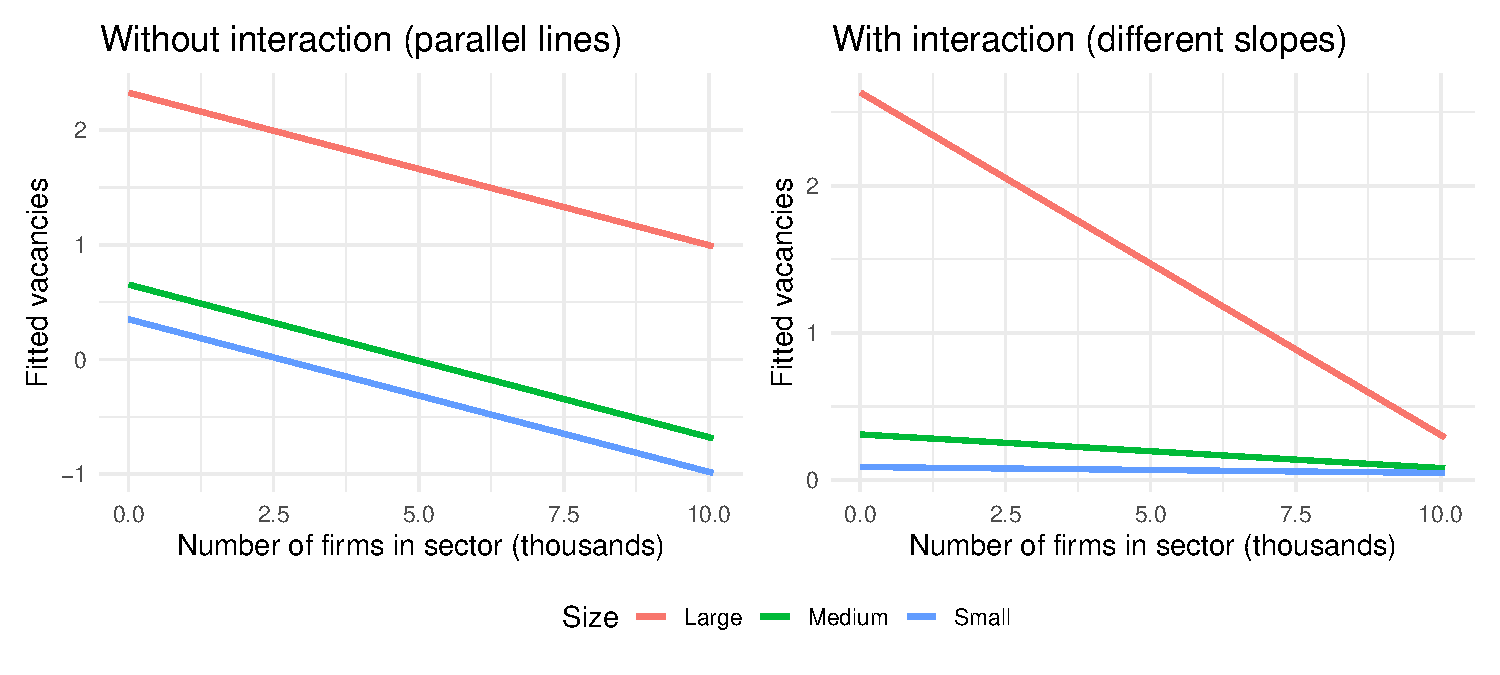
\includegraphics[width=\textwidth]{figs/cat-cont-interaction.pdf}
    \end{figure}

    \smallskip
    Testing the interaction ($H_0: \beta_4 = \beta_5 = 0$) is equivalent to testing whether the slopes are equal across groups.
\end{frame}

\subsection{Centering and scaling}

\begin{frame}{Why center?}
    In a model with interaction \texttt{Y $\sim$ group * x}:
    \begin{itemize}
        \item The ``main effect'' of \texttt{group} is the effect \textbf{when $x = 0$}
        \item If $x = 0$ is outside the observed range $\Rightarrow$ \alert{meaningless extrapolation}
    \end{itemize}

    \bigskip
    \textbf{Grand-mean centering:} replace $x$ with $x_c = x - \bar{x}$
    \begin{itemize}
        \item Now the main effect of \texttt{group} = effect \textbf{at the mean of $x$}
        \item Much more interpretable!
    \end{itemize}

    \bigskip
    \textbf{What changes and what stays the same:}
    \begin{table}[h]\centering\small
    \begin{tabular}{lcc}
    \hline
    & Centering & Standardisation \\
    \hline
    $R^2$, residuals, fitted values & \textbf{unchanged} & \textbf{unchanged} \\
    Interaction coefficients & \textbf{unchanged} & change (rescaled) \\
    Intercept, main-effect coefs & change & change \\
    \hline
    \end{tabular}
    \end{table}
\end{frame}

\begin{frame}{Scaling approaches -- supplementary material}
    For detailed examples with visualisations, centering vs.\ standardisation, and alternative scaling approaches, see \textbf{Supplementary notebook 07a: Interactions and scaling}.

    \bigskip
    Key additional topic: Gelman (2008) recommends:
    \begin{itemize}
        \item Divide \textbf{continuous} inputs by $2 \cdot \text{SD}$ (not $1 \cdot \text{SD}$)
        \item Center \textbf{binary} inputs by their mean
    \end{itemize}
    This makes coefficients of continuous and binary predictors directly comparable: a 1-unit change in the rescaled continuous variable represents moving from $1$ SD below to $1$ SD above the mean.
\end{frame}

\section{Marginal effects}

\begin{frame}{Marginal effects}
    What are marginal effects?
    \begin{figure}
        \centering
        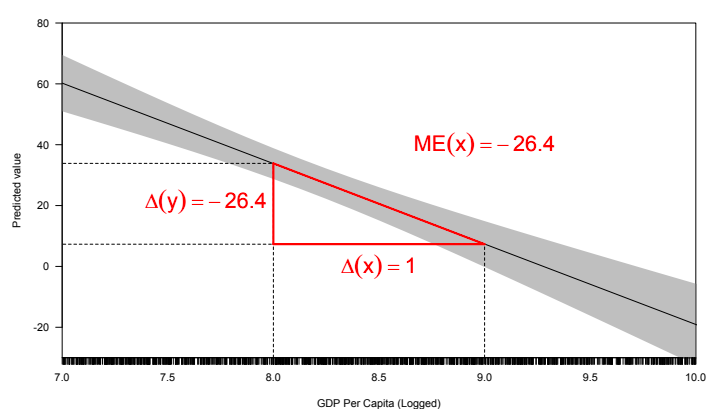
\includegraphics[width=0.7\textwidth]{figs/margin.png}
        \caption{Visualisation of marginal effect}
    \end{figure}
\end{frame}

\begin{frame}{Marginal effects  -- definition}
Marginal effect is defined as follows
\begin{equation}
    ME(x_{j}) = \frac{\partial\, E[y \mid \mathbf{x}]}{\partial\, x_{j}}
\end{equation}
For example, assume that $y = \beta_0 + \beta_1x_1 + \beta_2x_2 + \epsilon$. Then marginal effect for $x_1$ is equal to
\begin{equation}
    ME(x_1) = \frac{\partial (\beta_0 + \beta_1x_1 + \beta_2x_2)}{\partial x_1} = \beta_1.
\end{equation}
\end{frame}

\begin{frame}{Marginal effects -- examples}
\small
\begin{table}[ht]
\centering
\begin{tabular}{clcc}
  \hline
  & \textbf{Regression equation} & \textbf{ME w.r.t.} & \textbf{Formula} \\
  \hline
  (1) & $\hat{Y} = \beta_0 + \beta_1 X_1 + \beta_2 X_2 + \beta_3 X_1 X_2$
      & $X_1$ & $\beta_1 + \beta_3 X_2$ \\
      & & $X_2$ & $\beta_2 + \beta_3 X_1$ \\[6pt]
  (2) & $\hat{Y} = \beta_0 + \beta_1 X_1 + \beta_2 X^2_1 + \beta_3 X_2$
      & $X_1$ & $\beta_1 + 2\beta_2 X_1$ \\
      & & $X_2$ & $\beta_3$ \\[6pt]
  (3) & $\hat{Y} = \beta_0 + \beta_1 X_1 + \beta_2 X_2 +$
      & $X_1$ & $\beta_1 + \beta_4 X_2 +$ \\
      & $\beta_3 X_3 + \beta_4 X_1 X_2 +$ & & $\beta_6 X_3 + \beta_7 X_2 X_3$ \\
      & $\beta_5 X_2 X_3 + \beta_6 X_1 X_3 +$ & $X_2$ & $\beta_2 + \beta_4 X_1 +$ \\
      & $\beta_7 X_1 X_2 X_3$ & & $\beta_5 X_3 + \beta_7 X_1 X_3$ \\
      & & $X_3$ & $\beta_3 + \beta_5 X_2 +$ \\
      & & & $\beta_6 X_1 + \beta_7 X_1 X_2$ \\
  \hline
\end{tabular}
\end{table}

In models with interactions or polynomial terms, marginal effects depend on the values of other variables -- they are no longer constant.
\end{frame}

\begin{frame}{Marginal effects}
\begin{center}
    \Large

    How to calculate a unit change (marginal effect) of a given variable on the target variable?

\end{center}
\end{frame}

\begin{frame}{Calculations of marginal effects}
There are several ways to tackle this problem, the most popular are:

\begin{itemize}
    \item Average Marginal Effects (AME),
    \item Marginal Effects at the Mean / Median (MEM),
    \item Marginal Effects at  Representative Values (MERV).
\end{itemize}

\end{frame}

\begin{frame}{Average Marginal Effects}
    \begin{figure}
        \centering
        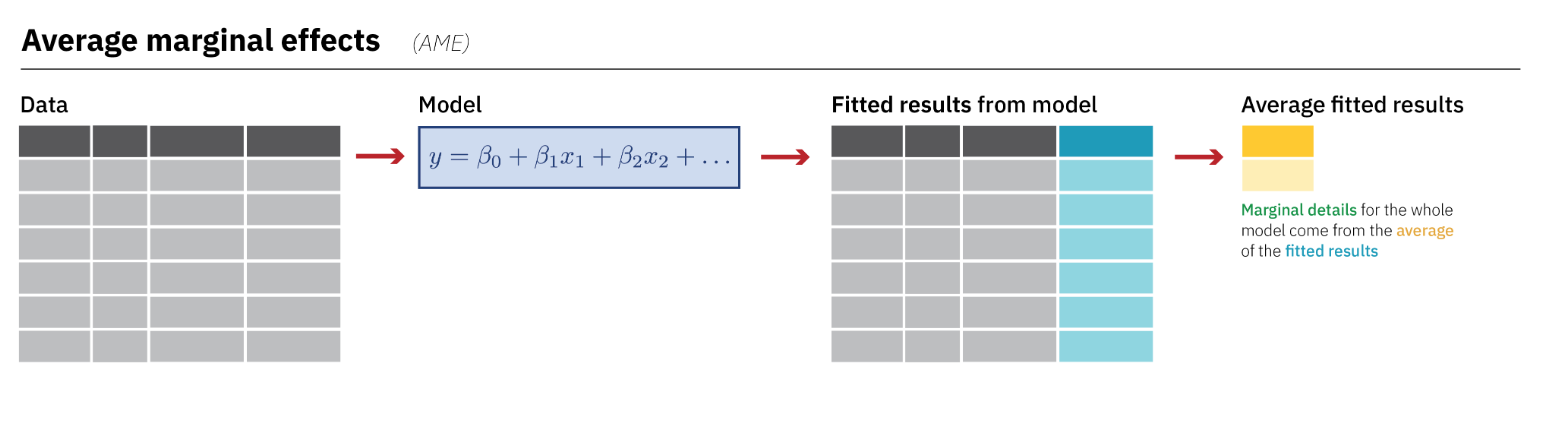
\includegraphics[width=\textwidth]{figs/ame.png}
        Source: \texttt{marginaleffects} package (\url{https://vincentarelbundock.github.io/marginaleffects/articles/slopes.html}).
    \end{figure}
\end{frame}

\begin{frame}{Marginal Effects at the Mean}
    \begin{figure}
        \centering
        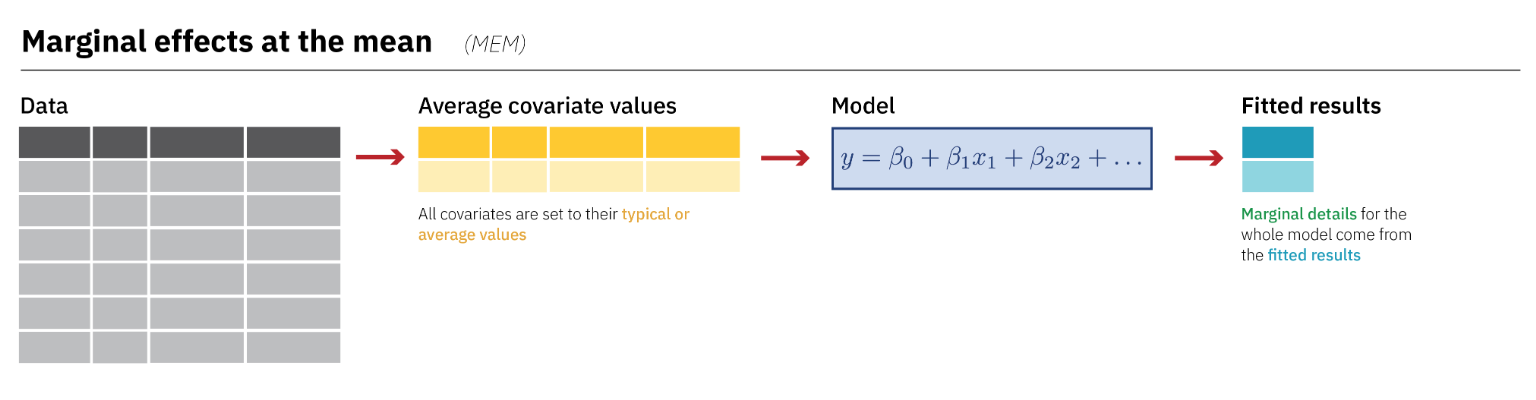
\includegraphics[width=\textwidth]{figs/mem.png}
        Source: \texttt{marginaleffects} package (\url{https://vincentarelbundock.github.io/marginaleffects/articles/slopes.html}).
    \end{figure}
\end{frame}

\begin{frame}{Marginal Effects at  Representative Values}
    \begin{figure}
        \centering
        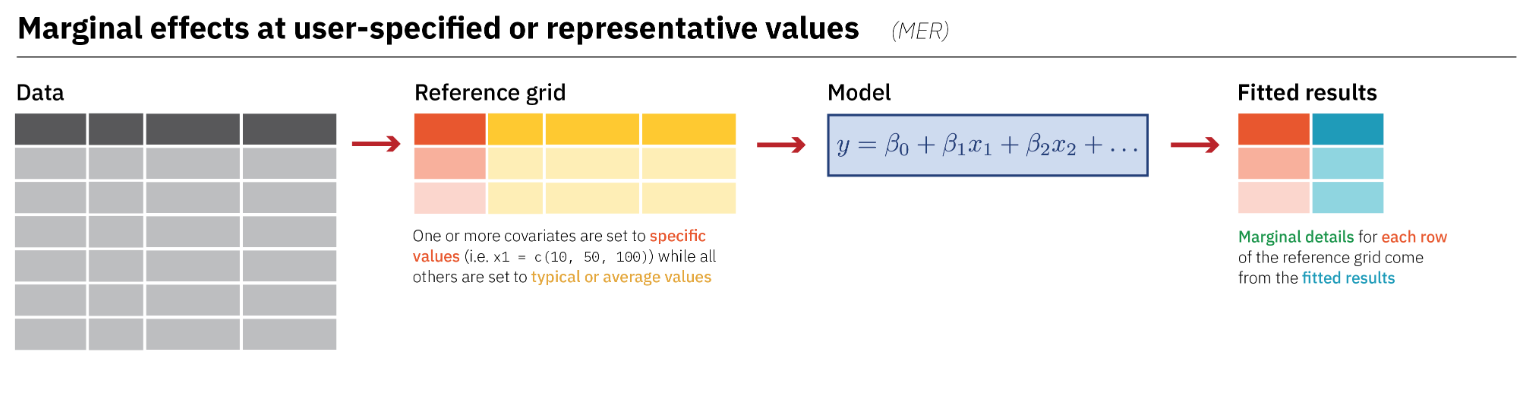
\includegraphics[width=\textwidth]{figs/merv.png}
        Source: \texttt{marginaleffects} package (\url{https://vincentarelbundock.github.io/marginaleffects/articles/slopes.html}).
    \end{figure}
\end{frame}

\begin{frame}{What about ML?}
\begin{figure}
    \centering
    
\includegraphics[width=\textwidth]{figs/biecek-book.png}
\end{figure}
\end{frame}

\begin{frame}{Practice -- marginal effects}
      \begin{table}[]
        \centering
        \caption{Overview of functions}
        %\label{tab:my_label}
        \begin{tabular}{cp{3cm}p{2cm}p{2cm}}
        \hline
          \textbf{Language}   & \textbf{R} &  \textbf{Python} & \textbf{Julia} \\
        \hline
         Packages  &
         marginaleffects &  marginaleffects & Effects.jl \\
        Functions &
         \texttt{avg\_slopes()}  & \texttt{avg\_slopes()} & effects \\
        \hline
        \end{tabular}
    \end{table}

    \medskip
    \small For a comprehensive guide, see Arel-Bundock et al.\ (2024).
\end{frame}

\begin{frame}{Marginal effects -- practice}

\begin{center}
Now, proceed to the example
\end{center}

\end{frame}

\begin{frame}[noframenumbering]{References}
\tiny
\begin{itemize}
\item Arel-Bundock, V., Greifer, N., \& Heiss, A. (2024). How to Interpret Statistical Models Using marginaleffects for R and Python. \textit{Journal of Statistical Software}, 111(9), 1--32.
\item Gelman, A. (2008). Scaling regression inputs by dividing by two standard deviations. \textit{Statistics in Medicine}, 27(15), 2865--2873.
\item Langsrud, {\O}. (2003). ANOVA for unbalanced data: Use Type II instead of Type III sums of squares. \textit{Statistics and Computing}, 13, 163--167.
\item Schad, D. J., Vasishth, S., Hohenstein, S., \& Kliegl, R. (2020). How to capitalize on a priori contrasts in linear (mixed) models: A tutorial. \textit{Journal of Memory and Language}, 110, 104038.
\item Wilkinson, G. N. \& Rogers, C. E. (1973). Symbolic description of factorial models for analysis of variance. \textit{Journal of the Royal Statistical Society C}, 22(3), 392--399.
\end{itemize}
\end{frame}

\section{Generalized linear models}

\subsection{Count data}

\begin{frame}{Vacancies: a count with lots of zeros}
We want to model the number of job vacancies $Y_i$ posted by firm $i$.

\medskip
\textbf{What kind of variable is $Y$?}
\begin{itemize}
    \justifying
    \item Non-negative integers: $Y_i \in \{0, 1, 2, \ldots\}$.
    \item In the JVS data: $\bar{Y} = 1.02$, \quad $s_Y^2 = 95.9$, \quad about $80\%$ of firms post zero vacancies.
    \item Variance is $\sim 100\times$ the mean -- not a Gaussian situation.
\end{itemize}

\medskip
\textbf{Goal.} Explain how $E[Y \mid X]$ varies with firm size, sector, ownership, region.

\medskip
\textbf{Question.} Why not just use linear regression?
\end{frame}


\begin{frame}{OLS problem 1: predictions can go negative}
The OLS specification:
\[
Y_i = \beta_0 + \mathbf{x}_i^\top\boldsymbol{\beta} + \varepsilon_i, \qquad \varepsilon_i \sim \mathcal{N}(0,\sigma^2).
\]

\medskip
The fitted mean $\hat{\mu}_i = \mathbf{x}_i^\top\hat{\boldsymbol{\beta}}$ lives on the entire real line.

\medskip
\textbf{Concretely.} Fit \texttt{vacancies $\sim$ size + public + nace}. For sub-groups with very low expected counts -- e.g.\ \emph{Small, private firms in a low-vacancy NACE division} -- OLS happily returns $\hat{\mu}_i < 0$.

\medskip
\alert{A negative count is impossible.} The model is fitting numbers it cannot mean.
\end{frame}


\begin{frame}{OLS problem 2: the variance is wrong}
For counts, the conditional variance \emph{grows with the conditional mean}. Poisson is the canonical case:
\[
\operatorname{Var}(Y \mid X) = E(Y \mid X).
\]

\medskip
OLS assumes the opposite -- a constant residual variance:
\[
\operatorname{Var}(\varepsilon_i) = \sigma^2 \quad \text{regardless of } \mathbf{x}_i.
\]

\medskip
\textbf{Consequence.} Standard errors and $p$-values from OLS are systematically wrong: too small where $\mu_i$ is large, too large where $\mu_i$ is small. Inference is unreliable.
\end{frame}


\begin{frame}{OLS problem 3: the distribution is wrong}
Likelihood-based inference (exact $t/F$, LR tests, AIC, prediction intervals) assumes the Gaussian likelihood -- which doesn't describe count residuals.

\medskip
The residuals from a count model are:
\begin{itemize}
    \justifying
    \item integer-valued,
    \item heavily right-skewed (a few firms post 50+ vacancies),
    \item with a large point mass at $0$ ($\sim 80\%$ of firms).
\end{itemize}

\medskip
OLS point estimates remain consistent for the linear approximation to $E[Y \mid X]$, and Wald CIs from robust (HC) SEs stay asymptotically valid -- but the likelihood-based machinery (LR, AIC, normal-theory prediction intervals) is misspecified.

\medskip
\textbf{Three strikes for OLS} -- predictions, variance, distribution. We need a different model.
\end{frame}


\begin{frame}{The popular shortcut: \texttt{log(y+1)}}
A textbook workaround. Add a constant to allow logging zeros:
\[
\log(Y_i + c) \;=\; \mathbf{x}_i^\top \boldsymbol{\beta} + \varepsilon_i, \qquad c \in \{1,\, 0.5,\, 0.001,\, \ldots\}.
\]

\medskip
\textbf{Why it looks attractive:}
\begin{itemize}
    \justifying
    \item Sidesteps $\log(0)$.
    \item Predictions on the original scale, $\exp(\mathbf{x}_i^\top\hat{\boldsymbol{\beta}}) - c$, are positive.
    \item Coefficients have a multiplicative ``elasticity'' feel.
\end{itemize}

\medskip
\textbf{And yet} -- the next two slides show three serious problems with it.
\end{frame}


\begin{frame}{Why \texttt{log(y+c)} fails (1/2)}
\textbf{Problem 1 -- the constant is arbitrary.}
\begin{itemize}
    \justifying
    \item Different conventional choices ($c = 1$ vs.\ $c = 0.5$ vs.\ $c = 0.001$) give \emph{different} $\hat{\boldsymbol{\beta}}$ and different $p$-values.
    \item There is no principled rule for picking $c$. Inference depends on a knob you cannot tune from the data.
\end{itemize}

\medskip
\textbf{Problem 2 -- it estimates the wrong thing.}
\begin{itemize}
    \justifying
    \item OLS targets $E\!\left[\log(Y+c) \mid X\right]$.
    \item Applied work usually wants $\log E[Y \mid X]$.
    \item By \textbf{Jensen's inequality}, the two differ. So $\exp(\hat{\beta}_j)$ is a \alert{biased} estimator of multiplicative effects on the mean.
\end{itemize}
\end{frame}


\begin{frame}{Why \texttt{log(y+c)} fails (2/2)}
\textbf{Problem 3 -- the zeros do not vanish.}
\begin{itemize}
    \justifying
    \item Before: $\sim 80\%$ of $Y_i$ equal $0$.
    \item After: $\sim 80\%$ of $\log(Y_i + c)$ equal $\log c$ -- still a point mass on the transformed scale.
    \item The non-Gaussian shape and heteroskedasticity carry over.
\end{itemize}

\medskip
\textbf{Bottom line.} \texttt{log(y+1)} relabels the problem rather than fixing it.

\medskip
\textbf{Better:} model $\log E[Y \mid X]$ directly with Poisson / NB regression -- next slide.

\medskip
\scriptsize References: O'Hara \& Kotze (2010), \textit{Methods Ecol.\ Evol.}; Bellégo, Benatia \& Pape (2022); Chen \& Roth (2024), \textit{QJE}; Wooldridge (1999), \textit{J.\ Econometrics}.
\end{frame}


\begin{frame}{The exponential mean model}
The right specification for a non-negative count:
\[
E(Y_i \mid \mathbf{x}_i) \;=\; \mu_i \;=\; \exp(\mathbf{x}_i^\top \boldsymbol{\beta}),
\qquad \text{i.e.} \qquad
\log \mu_i = \mathbf{x}_i^\top \boldsymbol{\beta}.
\]

\medskip
Two key properties:

\begin{itemize}
    \justifying
    \item \textbf{Predictions are non-negative.} $\mu_i > 0$ for every $\boldsymbol{\beta}$, by construction.
    \item \textbf{Coefficients are multiplicative.} A one-unit increase in $x_j$ multiplies $E[Y]$ by $\exp(\beta_j)$. For small $\beta_j$: $\exp(\beta_j) - 1 \approx \beta_j$ is a percentage change.
\end{itemize}

\medskip
The mean specification is shared by Poisson, quasi-Poisson, NB1, and NB2 -- they differ only in their \emph{variance} structure. We turn to that next.
\end{frame}


\begin{frame}{Count data -- standard distributions}
    \begin{itemize}
    \justifying
        \item The standard distribution for count data is the \textbf{Poisson} distribution:
        \[
        P(Y = y) = \frac{\mu^{y}\, \mathrm{e}^{-\mu}}{y!}, \quad y = 0, 1, 2, \ldots,
        \]
        with $E(Y) = \mu$ and $\operatorname{Var}(Y) = \mu$ (equidispersion).
        \item An alternative is the \textbf{Negative Binomial} (NB; mean parameterisation):
        \[
        P(Y = y) = \binom{y + k - 1}{y}\left(\frac{\mu}{\mu + k}\right)^{y}\left(\frac{k}{\mu + k}\right)^{k}, \quad y = 0, 1, 2, \ldots,
        \]
        with $E(Y) = \mu$ and $\operatorname{Var}(Y) = \mu + \mu^2/k$. The shape parameter $k$ controls overdispersion: $k \to \infty$ recovers the Poisson; small $k$ means more dispersion. (Some texts and \texttt{MASS::glm.nb} call this parameter $\theta$.)
        \item Other options: Geometric (NB with $k = 1$), Tweedie, zero-inflated, and hurdle distributions.
    \end{itemize}
\end{frame}


\begin{frame}{Count data -- more on the negative binomial}
The negative binomial (type 2) is a \textbf{gamma mixture of Poisson distributions}: $Y \mid \lambda \sim \text{Poisson}(\lambda)$ and $\lambda \sim \text{Gamma}(k,\, k/\mu)$ marginally yields
\[
P(Y = y) = \frac{\Gamma(y + k)}{\Gamma(k)\, y!} \cdot \frac{\mu^{y}\, k^{k}}{(\mu + k)^{y + k}}, \quad y = 0, 1, 2, \ldots,
\]
with mean $\mu$, shape $k$, and $\Gamma(\cdot)$ the gamma function.

\begin{itemize}
\justifying
    \item For \textbf{fixed} $k$, the model is a standard GLM (the natural parameter $\log\frac{\mu}{\mu+k}$ depends only on $\beta$).
    \item When $k$ is \textbf{estimated from the data}, the model technically falls outside the strict GLM framework. In practice, MLE is computed by alternating: hold $k$ fixed and update $\boldsymbol{\beta}$ via the GLM iteratively reweighted least squares (IRLS); then update $k$ from the score equation.
    \item Implemented in R as \texttt{MASS::glm.nb}; in Python as \texttt{statsmodels.discrete.NegativeBinomial}; in Julia via \texttt{GLM.jl} with \texttt{NegativeBinomial(k)} and a separate update for $k$.
\end{itemize}
\end{frame}


\begin{frame}{The Poisson assumption: equidispersion}
    \begin{itemize}
    \justifying
    \item The Poisson distribution imposes $E(Y) = \operatorname{Var}(Y)$ -- \textbf{equidispersion}.
    \item In economic applications we usually see $\operatorname{Var}(Y) > E(Y)$ -- \textbf{overdispersion}.
    \item Less commonly, we see $\operatorname{Var}(Y) < E(Y)$ -- \textbf{underdispersion}.
    \item For the JVS data, the marginal mean and variance of \texttt{vacancies} differ by two orders of magnitude:
\end{itemize}

\begin{table}[ht]
\centering
\caption{Mean and variance of the number of vacancies (JVS)}
\begin{tabular}{rr}
  \hline
  Mean & Variance \\
  \hline
  $1.02$ & $95.92$ \\
  \hline
\end{tabular}
\end{table}

\smallskip
\textbf{Implication.} A pure Poisson likelihood will produce SEs that are too small by a factor of roughly $\sqrt{\hat{\phi}} \approx \sqrt{95.92 / 1.02} \approx 9.7$ -- inference is severely anti-conservative unless we account for overdispersion.
\end{frame}

\begin{frame}{Count data -- where does overdispersion come from?}
Overdispersion typically reflects a failure of one of the Poisson assumptions:

\begin{itemize}
\justifying
    \item observations are \textbf{correlated} (e.g.\ clustered within firms, regions, or time);
    \item the event rate \textbf{is not constant} across units;
    \item rate variation is driven by \textbf{unobserved} or omitted predictors (latent heterogeneity).
\end{itemize}

\medskip
\textbf{Testing for overdispersion:}
\begin{itemize}
    \item R: \texttt{AER::dispersiontest()} (Cameron--Trivedi regression test); \texttt{performance::check\_overdispersion()}.
    \item Python: compare Pearson dispersion $\hat{\phi}$ to $1$, or fit a \texttt{NegativeBinomial} model and test whether $\alpha = 0$ (\texttt{statsmodels}).
    \item Julia: compute $\hat{\phi}$ manually from Pearson residuals; \texttt{GLM.jl} returns deviance and Pearson $\chi^2$.
\end{itemize}

\medskip
{\scriptsize Cameron, A.\,C.\ \& Trivedi, P.\,K.\ (1990). Regression-based tests for overdispersion in the Poisson model. \textit{Journal of Econometrics}, 46, 347--364.}

\end{frame}


\begin{frame}{Count data -- Poisson and NB regression}
    \begin{itemize}
    \justifying
        \item Poisson and NB regression both use the \textbf{log link}:
        \begin{equation}
            E(Y_{i} \mid \mathbf{x}_{i}) = \mu_{i} = \exp\!\left(\mathbf{x}_{i}^{\top} \boldsymbol{\beta}\right).
        \end{equation}
        \item To accommodate overdispersion ($\operatorname{Var}(Y) > E(Y)$), three options share the same conditional mean but differ in the assumed mean--variance relationship:
        \begin{itemize}
            \item \textbf{Quasi-Poisson} (QMLE, no full likelihood): $\operatorname{Var}(Y_i) = \phi\, \mu_i$ (linear). Estimate $\phi$ from Pearson residuals.
            \item \textbf{NB type 1} (NB1): $\operatorname{Var}(Y_i) = \mu_i + \mu_i / k = (1 + 1/k)\, \mu_i$ -- linear. Full likelihood; $k$ estimated by MLE.
            \item \textbf{NB type 2} (NB2): $\operatorname{Var}(Y_i) = \mu_i + \mu_i^2 / k$ -- quadratic in $\mu_i$. Full likelihood.
        \end{itemize}
        \item Quasi-Poisson and NB1 share a variance structure ($\operatorname{Var} = \phi\mu$ with $\phi = 1 + 1/k$) and yield numerically similar $\hat{\boldsymbol{\beta}}$, but the SEs are computed under different assumptions -- they are \textbf{not the same model}.
        \item \textbf{Pearson dispersion estimator} (used for quasi-Poisson and as a diagnostic):
        \[
        \hat{\phi} = \frac{1}{n - p}\sum_{i=1}^{n} \frac{(y_{i} - \hat{\mu}_{i})^{2}}{\hat{\mu}_{i}},
        \]
        with $n - p$ degrees of freedom. Values $\hat{\phi} \gg 1$ indicate overdispersion.
    \end{itemize}
\end{frame}




\begin{frame}{Count data -- fitting in practice}
\textbf{In R:}
\begin{itemize}
\justifying
    \item \texttt{glm(y \textasciitilde{} ..., family = poisson)} -- Poisson MLE; default \texttt{link = "log"}.
    \item \texttt{glm(y \textasciitilde{} ..., family = quasipoisson)} -- same $\hat{\boldsymbol{\beta}}$ as Poisson, with $\hat{\phi}$ inflating SEs.
    \item \texttt{glm(y \textasciitilde{} ..., family = MASS::negative.binomial(k))} -- NB with \emph{fixed} $k$ (not estimated). \texttt{negative.binomial(1)} is the geometric.
    \item \texttt{MASS::glm.nb(y \textasciitilde{} ...)} -- NB2 with $k$ \emph{estimated} from the data.
\end{itemize}

\medskip
\textbf{Python (\texttt{statsmodels}):}
\begin{itemize}
    \item \texttt{smf.glm(..., family=sm.families.Poisson())}
    \item \texttt{smf.glm(..., family=sm.families.NegativeBinomial(alpha=...))} -- $\alpha = 1/k$, fixed.
    \item \texttt{smf.negativebinomial(...).fit()} -- NB2 with $\alpha$ estimated.
\end{itemize}

\medskip
\textbf{Julia (\texttt{GLM.jl}):}
\begin{itemize}
    \item \texttt{glm(@formula(...), df, Poisson(), LogLink())}
    \item \texttt{negbin(@formula(...), df, LogLink())} -- estimates $k$.
\end{itemize}
\end{frame}



% \begin{frame}{Poisson regression -- warm-up}

% Please do the following exercise:

% \begin{enumerate}
%     \item Download the file \texttt{beers-glm-agg.csv} about beer consumption by single-person households in 2011 [file can be found on the \underline{moodle} platform, section \underline{Generalized linear models}].
%     \item Read the data into software of preference.
%     \item Fit Poisson regression where dependent variable is \textbf{beers} and independent variable is \textbf{klm}.
%     \item What you can tell about the consumption of beer between levels of \textbf{klm} variable (remember that this variable is a categorical variable)? 
% \end{enumerate}

% \end{frame}


\begin{frame}{Poisson regression -- plan for the lecture}

Is the model ok? but what do we mean by that? 
    \begin{itemize}
        \item How to detect and deal with overdispersion?
        \item How to visually assess the model?
        \item How to check which model (i.e. distribution) is better?
        \item How to report results using tables and plots?
    \end{itemize}
    
    \vspace{0.5cm}
    
    R Packages
    \begin{itemize}
    \item \texttt{car} -- \texttt{Anova} function to verify contribution of a given variable (not only the individual factor level).
    \item \texttt{boot} -- package distributed with R, function: \texttt{glm.diag.plots} which resembles \texttt{plot.lm} 
    \item \texttt{performance} -- \url{https://easystats.github.io/performance/}
    \item \texttt{sjPlot} -- \url{https://strengejacke.github.io/sjPlot/}
    \item \texttt{countreg::rootogram} -- \url{https://rdrr.io/rforge/countreg/}
\end{itemize}

\end{frame}

\begin{frame}{Poisson vs Negative Binomial}


\begin{quote}
(...) I'll also add that by default one should almost always use negative binomial models over the Poisson because the assumption of equidispersion is rarely actually met, but you anyway have to check which dispersion issues are present in the model first before deciding on which to use.

Reference

Hilbe, J. M. (2011). Negative binomial regression (2nd ed). Cambridge University Press.
\end{quote}

Source: Shawn Hemelstrand

\url{https://stats.stackexchange.com/questions/653727/when-to-use-negative-binomial-and-poisson-regression}
\end{frame}


\begin{frame}{Poisson vs Negative Binomial}


\begin{quote}
Poisson regression can be reframed a quasi-maximum likelihood (QMLE) model. That means as long as the relationship between the predictors and the outcome mean is correctly specified, the QMLE estimate of the coefficients is consistent, whether or not the outcome is actually Poisson distributed (including whether or not the outcome is over- or under-dispersed). 
\end{quote}

\begin{quote}
In contrast, the negative binomial (NB) model requires strong assumptions. If the outcome distribution is not negative binomial (e.g., it does not specifically follow the NB distribution or the dispersion is not accurately captured by the implied mean-variance relationship of the NB model, including if there is under-dispersion) the estimate isn't even consistent. 
\end{quote}

Source: Noah Greifer

\url{https://stats.stackexchange.com/questions/653727/when-to-use-negative-binomial-and-poisson-regression}
\end{frame}

\begin{frame}{Poisson vs Negative Binomial}
\begin{center}
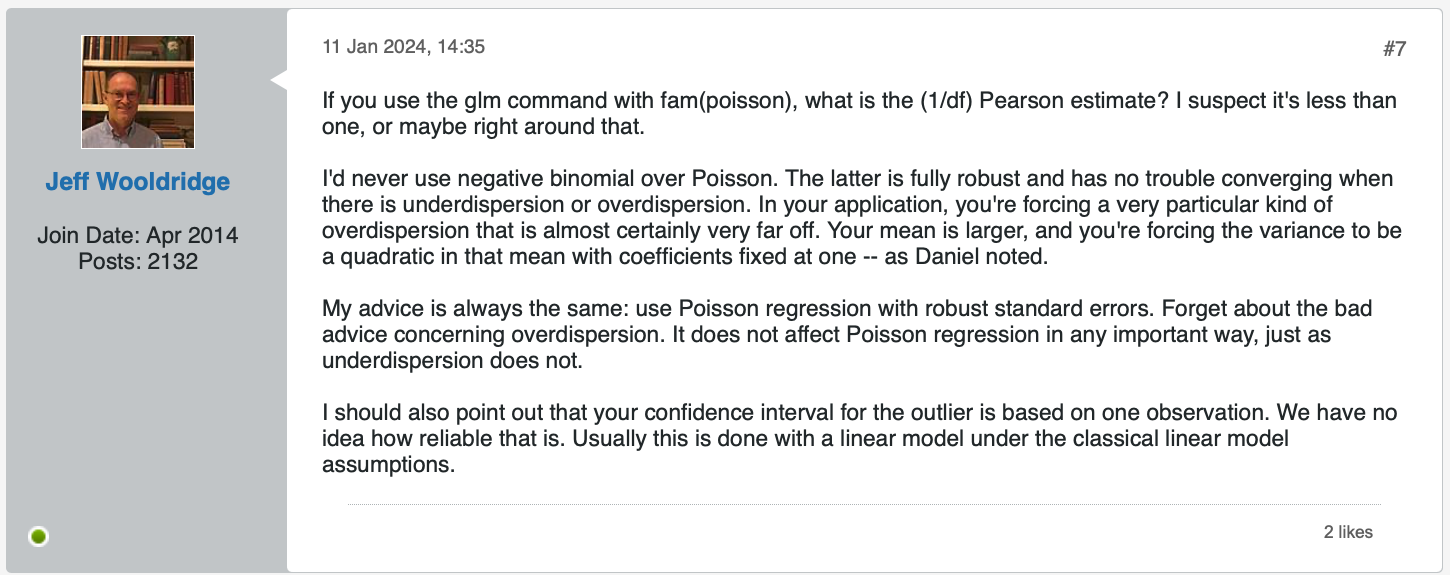
\includegraphics[width=\textwidth]{figs/jeff1.png}  
\end{center}
\end{frame}

\begin{frame}{Poisson vs Negative Binomial}
\begin{center}

\includegraphics[width=0.8\textwidth]{figs/jeff2.png}  
\end{center}
\end{frame}


\begin{frame}{Count data -- further reading}
    \begin{itemize}
        \item \textbf{More distributions} -- see package \texttt{VGAM} which implements a high number of discrete distributions (over 30).
        \item \textbf{Diagnostics} -- diagnostics for count regression models is crucial, see \texttt{DHARMa} package.
        \item \textbf{Robust standard errors} -- see \texttt{sandwich} package.
        \item \textbf{Variable selection} -- see \texttt{glmnet} package (LASSO and its extensions)
        \item \textbf{(Outlier) Robust inference} -- see \texttt{robustbase}, \texttt{robust} packages.
    \end{itemize}
\end{frame}

\begin{frame}{Count data -- practice}

\begin{center}
Now, proceed to the example of Poisson and NB regression. 
\end{center}


\end{frame}

\subsection{Binary outcomes}

\begin{frame}{Has vacancy: a binary outcome}
We want to model whether firm $i$ posts at least one job vacancy.
Define $Y_i = \mathbb{1}\{\texttt{vacancies}_i > 0\}$, so $Y_i \in \{0, 1\}$.

\medskip
\textbf{What kind of variable is $Y$?}
\begin{itemize}
    \justifying
    \item Bernoulli: $\pi_i = P(Y_i = 1 \mid \mathbf{x}_i)$, with $\operatorname{Var}(Y_i \mid \mathbf{x}_i) = \pi_i(1-\pi_i)$.
    \item In the JVS data: about $12\%$ of firms post at least one vacancy.
    \item No values outside $\{0,1\}$ -- not a Gaussian situation.
\end{itemize}

\medskip
\textbf{Goal.} Explain how $\pi_i = E[Y_i \mid \mathbf{x}_i]$ varies with firm size, sector, ownership, region.

\medskip
\textbf{Question.} Why not just use linear regression?
\end{frame}


\begin{frame}{LPM problem 1: predictions can leave $[0,1]$}
The linear probability model (LPM):
\[
P(Y_i = 1 \mid \mathbf{x}_i) = \beta_0 + \mathbf{x}_i^\top\bbeta.
\]

\medskip
The right-hand side lives on the entire real line; nothing prevents $\hat{\pi}_i < 0$ or $\hat{\pi}_i > 1$.

\medskip
\textbf{Concretely.} Fit \texttt{has\_vacancy $\sim$ size + public + nace}. For sub-groups with very low (or very high) base rates, OLS happily returns $\hat{\pi}_i$ outside $[0,1]$.

\medskip
\alert{Probabilities outside $[0,1]$ are not probabilities.} The model is fitting numbers it cannot mean.
\end{frame}


\begin{frame}{LPM problem 2: heteroskedasticity is built in}
For a Bernoulli outcome, the conditional variance is determined by the conditional mean:
\[
\operatorname{Var}(Y_i \mid \mathbf{x}_i) = \pi_i(1 - \pi_i).
\]

\medskip
This is non-constant and tied to $\mathbf{x}_i$ through $\pi_i$ -- LPM violates OLS's homoskedasticity assumption \emph{by construction}.

\medskip
\textbf{Consequence.} Standard errors and $p$-values from OLS are wrong unless we use robust (HC) SEs. Even then, the LPM target is only a linear approximation to a non-linear $\pi(\mathbf{x})$.
\end{frame}


\begin{frame}{LPM problem 3: the distribution is wrong}
Likelihood-based inference (exact $t/F$, LR tests, AIC, prediction intervals) assumes the Gaussian likelihood -- which doesn't describe binary residuals.

\medskip
The residuals from a binary model take only \emph{two values} for each $\mathbf{x}_i$:
\[
\varepsilon_i =
\begin{cases}
\phantom{-}1 - \hat{\pi}_i & \text{if } y_i = 1, \\[2pt]
-\hat{\pi}_i               & \text{if } y_i = 0.
\end{cases}
\]

\medskip
OLS point estimates remain consistent for the linear approximation to $\pi(\mathbf{x})$, and Wald CIs from robust (HC) SEs stay asymptotically valid -- but the likelihood-based machinery (LR, AIC, normal-theory prediction intervals) is misspecified.

\medskip
\textbf{Three strikes for OLS} -- range, variance, distribution. We need a different model.

\medskip
{\scriptsize \textit{Note.} The LPM is still used in applied econometrics for its interpretive simplicity (coefficients $=$ marginal effects on probability) -- but only with heteroskedasticity-robust SEs, and rarely for prediction.}
\end{frame}


\begin{frame}{Odds and log odds}
     \begin{itemize}
         \item For a binary response where $\pi = \Pr(\text{success})$, the odds of success are
         \begin{equation}
             \text{odds} = \frac{\pi}{1-\pi}.
         \end{equation}
         \item Taking logs, the log-odds (logit) vary symmetrically around 0:
         \begin{equation}
             \logit(\pi) = \log\left(\frac{\pi}{1-\pi}\right).
         \end{equation}
         \item Log odds
         \begin{itemize}
             \item Symmetric around $\pi = 0.5$; $\logit(\pi) = -\logit(1-\pi)$
             \item The logit transformation of probability provides the basis for logistic regression
         \end{itemize}
     \end{itemize}
 \end{frame}

 \begin{frame}{Odds ratios}

 \begin{itemize}
     \item For two groups with probabilities of success $\pi_1,\pi_2$, the odds ratio (denoted $\theta$) is the ratio of the two groups' odds:
     \begin{equation}
         \theta = \frac{\text{odds}_{1}}{\text{odds}_{2}} = \frac{\pi_{1}/(1-\pi_{1})}{\pi_{2}/(1-\pi_{2})}.
     \end{equation}
     \item In a $2\times 2$ table with joint cell probabilities $\pi_{ij}$ (row $i$ = group, column $j$ = outcome; $j{=}1$ success, $j{=}2$ failure), this equals the cross-product: $\theta = \pi_{11}\pi_{22}/(\pi_{12}\pi_{21})$.
     \item $\theta = 1$ -- independence, no association.
     \item More convenient is the log odds ratio $\psi = \log(\theta)$, symmetric around 0:
     \begin{equation}
         \psi = \log(\theta) = \logit(\pi_{1}) - \logit(\pi_{2}).
     \end{equation}
\end{itemize}
\end{frame}

\begin{frame}{Odds and odds ratio -- example}
    \begin{itemize}
        \item Consider the following example based on the data from the lecture
        \begin{table}
            \centering
            \begin{tabular}{lrr}
            \hline
                      & No vacancy & Has vacancy \\
            \hline
            Public    & 17{,}639   & 2{,}615     \\
            Private   & 32{,}912   & 4{,}314     \\
            \hline
            \end{tabular}
        \end{table}
    \item Let $\pi_{\text{Pub}}$ denote the probability that a~public entity has a~vacancy, and $\pi_{\text{Pri}}$ the same for a~private entity.
    \item Then we can calculate the odds as follows:
    $$
    \text{odds}_{\text{Pub}} = \frac{\pi_{\text{Pub}}}{1 - \pi_{\text{Pub}}} = \frac{2{,}615/20{,}254}{17{,}639/20{,}254} = 0.148, \quad \text{odds}_{\text{Pri}} = 0.131.
    $$
    \item The odds ratio is
    $$
    \theta = \frac{\text{odds}_{\text{Pub}}}{\text{odds}_{\text{Pri}}} = \frac{0.148}{0.131} = 1.13, \quad \theta^{-1} = 0.87.
    $$
    \end{itemize}
\end{frame}

\begin{frame}{Odds and odds ratio -- interpretation}
    \begin{itemize}
        \item Public: the odds of having at least one vacancy are about $0.148$ (roughly $1{:}6.7$).
        \item Private: the odds of having at least one vacancy are about $0.131$ (roughly $1{:}7.6$).
        \item Public vs.\ Private: the odds are about $13\%$ higher for public entities than for private ones ($\theta = 1.13$).
    \end{itemize}
\end{frame}

\begin{frame}{Odds and odds ratio -- general rule of interpretation}
    \begin{itemize}
        \item If $\theta = 1$, the odds of having a~vacancy are the same for public and private entities -- no association.
        \item If $\theta > 1$, the odds of having a~vacancy are higher for public than for private entities -- positive association.
        \item If $\theta < 1$, the odds of having a~vacancy are lower for public than for private entities -- negative association.
    \end{itemize}
\end{frame}

\begin{frame}{Logistic regression: the logit specification}
Model the log-odds as a linear function of covariates:
\[
\logit(\pi_i) = \log\!\frac{\pi_i}{1 - \pi_i} = \beta_0 + \mathbf{x}_i^\top\bbeta.
\]

\medskip
\textbf{Why the logit?}
\begin{itemize}
    \justifying
    \item Maps $\pi_i \in (0,1)$ to $\eta_i \in (-\infty, \infty)$ -- the right scale for a linear predictor.
    \item Solving for $\pi_i$ gives the inverse-logit (logistic CDF):
    \[
    \pi_i = \frac{\exp(\beta_0 + \mathbf{x}_i^\top\bbeta)}{1 + \exp(\beta_0 + \mathbf{x}_i^\top\bbeta)} \;=\; \Lambda(\beta_0 + \mathbf{x}_i^\top\bbeta).
    \]
    \item Predictions $\hat{\pi}_i \in (0,1)$ \emph{by construction} -- fixing LPM's problem~1.
\end{itemize}
\end{frame}


\begin{frame}{Coefficients as log odds ratios}
A one-unit increase in $X_j$ (others fixed) shifts the linear predictor by $\beta_j$. Since $\eta_i = \logit(\pi_i)$, this is a change in log-odds:
\[
\beta_j \;=\; \logit(\pi_{+}) - \logit(\pi_{-}) \;=\; \log\!\frac{\pi_+/(1-\pi_+)}{\pi_-/(1-\pi_-)} \;=\; \log\theta_j,
\]
where $\pi_-, \pi_+$ are success probabilities at $X_j = x$ and $X_j = x+1$.

\medskip
\textbf{Two reading modes:}
\begin{itemize}
    \justifying
    \item $\hat{\beta}_j$ -- log odds ratio for a unit change in $X_j$.
    \item $\exp(\hat{\beta}_j)$ -- odds ratio. E.g.\ $\exp(\hat{\beta}_j) = 1.13 \Rightarrow$ odds are $13\%$ higher.
\end{itemize}

\medskip
The OR machinery from earlier slides is exactly what every logistic-regression coefficient measures.
\end{frame}


\begin{frame}{Other links: probit and cloglog}
A binary GLM uses a link $g$ such that $g(\pi_i) = \beta_0 + \mathbf{x}_i^\top\bbeta$:

\begin{itemize}
    \justifying
    \item \textbf{logit:} $g(\pi) = \log\frac{\pi}{1-\pi}$, so $\pi = \Lambda(\eta) = \dfrac{e^\eta}{1+e^\eta}$.
    \item \textbf{probit:} $g(\pi) = \Phi^{-1}(\pi)$, so $\pi = \Phi(\eta)$, where $\Phi$ is the standard normal CDF.
    \item \textbf{cloglog:} $g(\pi) = \log(-\log(1-\pi))$, so $\pi = 1 - \exp(-\exp(\eta))$. Asymmetric -- typically used when the positive (or negative) outcome is rare.
\end{itemize}

\medskip
Logit and probit produce very similar fitted probabilities (probit coefficients $\approx \beta^{\text{logit}}/1.6$); the choice rarely matters for predictions but does matter for interpretation -- only the logit gives log-odds-ratio coefficients.
\end{frame}


\begin{frame}{Estimation by maximum likelihood}
With $Y_i \mid \mathbf{x}_i \sim \text{Bernoulli}(\pi_i)$ and $\pi_i = \Lambda(\eta_i)$, the log-likelihood is
\[
\ell(\bbeta) = \sum_{i=1}^n \left[\, y_i\, \eta_i - \log(1 + e^{\eta_i}) \,\right], \qquad \eta_i = \beta_0 + \mathbf{x}_i^\top\bbeta.
\]

\medskip
\textbf{Properties:}
\begin{itemize}
    \justifying
    \item Concave in $\bbeta$ -- a unique global maximum (when it exists; complete separation is the failure case).
    \item No closed form. Solved by Newton--Raphson / iteratively reweighted least squares (IRLS), the standard fitting routine for GLMs.
    \item Inference: Wald, likelihood-ratio, and score tests -- asymptotically equivalent under regularity.
\end{itemize}

\medskip
\textbf{Implementations.} R: \texttt{glm(..., family = binomial)}; Python: \texttt{statsmodels.Logit}; Julia: \texttt{glm(..., Bernoulli(), LogitLink())}.
\end{frame}

\begin{frame}{Marginal effects for logistic regression}
    \begin{itemize}
        \item Coefficients $\beta_j$ in logistic, probit or cloglog models live on the link scale (log-odds, $z$-score, etc.) -- they do not directly give changes in $P(Y=1)$.
        \item \textbf{Marginal effects} translate $\beta_j$ to the probability scale.
        \item By the chain rule, $\partial \pi_i/\partial x_{ij} = g(\eta_i)\,\beta_j$, where $\eta_i = \beta_0 + \mathbf{x}_i^\top\bbeta$ and $g(\cdot)$ is the density associated with the chosen link: logistic for logit, standard normal for probit. We interpret results in terms of densities multiplied by the estimated $\beta$.
    \end{itemize}
\end{frame}


\begin{frame}{Marginal effects for logistic regression}
\begin{itemize}
    \item Let $p(\mathbf{x}_i) = P(Y_i = 1 \mid \mathbf{x}_i) = G(\beta_0 + \mathbf{x}_i^\top\bbeta)$, where $G(\cdot)$ is the inverse link (logistic CDF, normal CDF, or other), satisfying $0 < G(z) < 1$ for all real $z$.
    \item Then the marginal effect of the $j$-th covariate is

    $$
    \frac{\partial p(\mathbf{x}_i)}{\partial x_{ij}} = g\!\left(\beta_0 + \mathbf{x}_i^\top\bbeta\right)\beta_j, \quad \text{where } g(z) \equiv \frac{dG}{dz}(z).
    $$
    \item $g(z)$ for logit is $\exp(z)/[1+\exp(z)]^2$, the PDF of the standard logistic distribution.
    \item $g(z)$ for probit is $\phi(z)$, the PDF of the standard normal distribution.
\end{itemize}
\end{frame}


\begin{frame}{Three flavors of marginal effect}
The marginal effect $g(\eta_i)\,\beta_j$ depends on $\eta_i$ -- so it varies across observations. Three common ways to summarise:

\begin{itemize}
    \justifying
    \item \textbf{Average marginal effect (AME):} average over the sample,
    \[
    \widehat{\text{AME}}_j = \frac{1}{n}\sum_{i=1}^n g(\hat{\eta}_i)\,\hat{\beta}_j.
    \]
    Default in \texttt{marginaleffects}, \texttt{statsmodels}, Stata's \texttt{margins, dydx(*)}.
    \item \textbf{Marginal effect at the mean (MEM):} evaluate at $\bar{\mathbf{x}}$,
    $\widehat{\text{MEM}}_j = g(\hat{\beta}_0 + \bar{\mathbf{x}}^\top\hat{\bbeta})\,\hat{\beta}_j$. Older default; ill-defined when $\bar{\mathbf{x}}$ averages dummies.
    \item \textbf{Marginal effect at representative values (MER):} evaluate at user-chosen $\mathbf{x}^\star$. Useful for counterfactuals and group comparisons.
\end{itemize}

\medskip
For most reporting, the AME is the default choice.
\end{frame}


\begin{frame}[fragile]{Marginal effects: example}
Logistic regression \texttt{has\_vacancy $\sim$ public}.

\smallskip
\textbf{Coefficients (link scale):}
\begin{table}[ht]
\centering
\begin{tabular}{lrrr}
\hline
                                     & Estimate & Std.\ Error & $\exp(\hat{\beta})$ \\
\hline
$\hat{\beta}_0$ (Private baseline)   & $-2.034$ & $0.017$     & --                   \\
$\hat{\beta}_1$ (Public, log OR)     & $\phantom{-}0.122$  & $0.027$     & $1.130$              \\
\hline
\end{tabular}
\end{table}
Log-odds for public are $0.122$ above private; equivalently, odds are $13\%$ higher.

\medskip
\textbf{Average marginal effect (probability scale):}
\begin{table}[ht]
\centering
\begin{tabular}{llrrrr}
\hline
Term   & Contrast & Estimate & Std.\ Error & Statistic & p-value   \\
\hline
public & $1 - 0$  & $0.0132$ & $0.0029$    & $4.59$    & $<\!0.001$ \\
\hline
\end{tabular}
\end{table}
Public firms are about $1.3$ p.p.\ more likely to post at least one vacancy -- noticeable next to a baseline rate of $\sim\!12\%$.
\end{frame}


\begin{frame}{Goodness of fit and model comparison}
\textbf{Likelihood-based:}
\begin{itemize}
    \justifying
    \item \textbf{Deviance:} $D = 2\!\left[\ell(\text{saturated}) - \ell(\hat{\bbeta})\right]$. For nested models, $D_{\text{reduced}} - D_{\text{full}} \sim \chi^2_{\Delta p}$ asymptotically -- the LR test.
    \item \textbf{AIC / BIC:} for non-nested model comparison; lower is better.
    \item \textbf{Pseudo-$R^2$} (McFadden, Cox--Snell, Nagelkerke, Tjur): \emph{not} OLS's $R^2$. Useful only for ranking models on the same data.
\end{itemize}

\medskip
\textbf{Hosmer--Lemeshow test:} bin observations by $\hat{\pi}_i$, compare observed vs.\ expected counts in each bin via $\chi^2$. Sensitive to bin choice; modern alternatives prefer calibration plots.
\end{frame}


\begin{frame}{Discrimination and calibration}
\textbf{Discrimination -- can the model separate $Y=1$ from $Y=0$?}
\begin{itemize}
    \justifying
    \item Pick a threshold $c$, predict $\hat{Y}_i = \mathbb{1}\{\hat{\pi}_i > c\}$ -- yields a confusion matrix.
    \item \textbf{ROC curve:} TPR vs.\ FPR over all $c$. \textbf{AUC} = area under it; $0.5$ = random, $1$ = perfect.
\end{itemize}

\medskip
\textbf{Calibration -- are predicted probabilities at the right level?}
\begin{itemize}
    \justifying
    \item Plot observed proportion vs.\ $\hat{\pi}_i$ (deciles or smooth).
    \item A well-calibrated model lies on the $45^\circ$ line.
\end{itemize}

\medskip
A model can have high AUC (good ranking) yet be poorly calibrated (wrong levels) -- always check both.
\end{frame}


\begin{frame}{Logistic regression -- in practice}
\textbf{R}
\begin{itemize}
    \justifying
    \item \texttt{glm(y \textasciitilde{} ..., family = binomial)} -- default link is \texttt{logit}.
    \item Alternative links: \texttt{binomial("probit")}, \texttt{binomial("cloglog")}.
    \item \texttt{marginaleffects::avg\_slopes()} -- AMEs with delta-method SEs.
    \item \texttt{performance::performance()} -- pseudo-$R^2$, AUC, calibration checks.
    \item \texttt{pROC} / \texttt{ROCR} -- ROC curves and AUC.
    \item \texttt{DHARMa} -- residual diagnostics for binomial GLMs.
\end{itemize}

\medskip
\textbf{Python (\texttt{statsmodels}):}
\begin{itemize}
    \justifying
    \item \texttt{smf.logit(formula, data).fit()} -- Bernoulli/logit MLE.
    \item Equivalently: \texttt{smf.glm(..., family=sm.families.Binomial())}.
    \item \texttt{result.get\_margeff(at='overall').summary()} -- AMEs.
\end{itemize}

\medskip
\textbf{Julia (\texttt{GLM.jl}):}
\begin{itemize}
    \justifying
    \item \texttt{glm(@formula(...), df, Bernoulli(), LogitLink())}.
    \item \texttt{Effects.jl} for marginal effects.
\end{itemize}
\end{frame}


\begin{frame}{Logistic regression -- practice}
\begin{center}
Now, proceed to the example of logistic regression.
\end{center}
\end{frame}

\section{Classification and regression trees}

\subsection{Motivation}

\begin{frame}{Beyond GLM: questions a tree can answer}
We have just modelled two outcomes from the JVS data:
\begin{itemize}
    \justifying
    \item \texttt{vacancies} -- a count (Poisson / NB regression, \S 11.1).
    \item \texttt{has\_vacancy} = $\mathbb{I}(\texttt{vacancies} > 0)$ -- a binary outcome (logistic regression, \S 11.2).
\end{itemize}

\medskip
\textbf{What is hard for a GLM here?}
\begin{itemize}
    \justifying
    \item Strongly non-linear effects of firm \texttt{size}, sector, region.
    \item High-order interactions (e.g.\ \texttt{size} $\times$ \texttt{nace} $\times$ \texttt{woj}) -- writing them out explodes the design matrix.
    \item Many small categories: \texttt{nace\_division} has $\approx 90$ levels, most rarely populated.
\end{itemize}

\medskip
\textbf{Question.} Is there a model that picks the relevant variables, interactions, and cut-points \emph{automatically} from the data?
\end{frame}


\begin{frame}{A different modelling philosophy}
Breiman (2001, \textit{Statistical Science}) called this the \emph{two cultures}:
\begin{itemize}
    \justifying
    \item \textbf{Data-modelling culture} -- assume $Y \mid X \sim$ (some distribution) with a link and a linear predictor; estimate parameters; do inference. (OLS, GLM.)
    \item \textbf{Algorithmic culture} -- treat $f(X) = E[Y \mid X]$ as an unknown function; learn it from the data with as few parametric assumptions as possible. (Trees, random forests, boosting, neural nets, $\ldots$)
\end{itemize}

\medskip
\textbf{What does a tree assume?}
\begin{itemize}
    \justifying
    \item \emph{No} link function, \emph{no} variance function, \emph{no} parametric form for $E[Y \mid X]$.
    \item Approximate $f(X)$ by a \textbf{piecewise constant} function on a partition of the predictor space into rectangular regions $R_1, \ldots, R_M$:
    \[
        \hat f(\bx) \;=\; \sum_{m=1}^{M} \hat c_m \,\mathbb{I}(\bx \in R_m).
    \]
    \item For \textbf{regression}, $\hat c_m = \bar y_{R_m}$; for \textbf{classification}, $\hat c_m$ is the class-probability vector / majority class in $R_m$.
\end{itemize}
\end{frame}


\begin{frame}{One picture vs.\ one regression table}
\textbf{Logistic regression} of \texttt{has\_vacancy}:
\[
\logit \Pr(Y=1 \mid \bx) = \beta_0 + \beta_1 \,\texttt{size}_M + \beta_2 \,\texttt{size}_L + \beta_3 \,\texttt{public} + \ldots
\]
$\Rightarrow$ a \emph{table} of coefficients; effects are additive on the log-odds scale.

\medskip
\textbf{Tree} for the same outcome:
$\Rightarrow$ a \emph{sequence of yes/no questions} -- ``is the firm large? if so, is it private?'' -- ending in a predicted probability.

\medskip
The two objects are \alert{not directly comparable}: one returns coefficients on a scale, the other returns a decision rule. The next slide shows a concrete tree on the JVS data.
\end{frame}


\subsection{Recursive partitioning}

\begin{frame}{Toy classification tree -- \texttt{has\_vacancy} on JVS}
\centering
\begin{tikzpicture}[
    >=stealth, thick,
    every node/.style={font=\small},
    internal/.style={draw, rectangle, rounded corners=2pt, align=center, inner sep=4pt},
    leaf/.style={draw, rectangle, rounded corners=6pt, fill=blue!7, align=center, inner sep=4pt},
    level 1/.style={sibling distance=55mm, level distance=14mm},
    level 2/.style={sibling distance=32mm, level distance=14mm}
]
\node[internal] {\texttt{size} = Large?}
    child {node[leaf] {Small / Medium\\$n=29\,639$\\$\hat p = 0.067$}
        edge from parent node[above left] {no}}
    child {node[internal] {\texttt{public} = 1?}
        child {node[leaf] {Large, private\\$n=15\,873$\\$\hat p = 0.186$}
            edge from parent node[above left] {no}}
        child {node[leaf] {Large, public\\$n=11\,968$\\$\hat p = 0.166$}
            edge from parent node[above right] {yes}}
        edge from parent node[above right] {yes}};
\end{tikzpicture}

\medskip
Each \textbf{leaf} reports the count $n$ and the predicted probability $\hat p = \Pr(\texttt{has\_vacancy} = 1)$. To classify a new firm, walk from the root down and read off $\hat p$.
\end{frame}


\begin{frame}{Same tree, regression target}
The \emph{same partition} can be used to predict the count \texttt{vacancies}: only the leaf summary changes.

\medskip
\centering
\begin{tikzpicture}[
    >=stealth, thick,
    every node/.style={font=\small},
    internal/.style={draw, rectangle, rounded corners=2pt, align=center, inner sep=4pt},
    leaf/.style={draw, rectangle, rounded corners=6pt, fill=orange!10, align=center, inner sep=4pt},
    level 1/.style={sibling distance=55mm, level distance=14mm},
    level 2/.style={sibling distance=32mm, level distance=14mm}
]
\node[internal] {\texttt{size} = Large?}
    child {node[leaf] {Small / Medium\\$n=29\,639$\\$\bar y = 0.17$}
        edge from parent node[above left] {no}}
    child {node[internal] {\texttt{public} = 1?}
        child {node[leaf] {Large, private\\$n=15\,873$\\$\bar y = 2.44$}
            edge from parent node[above left] {no}}
        child {node[leaf] {Large, public\\$n=11\,968$\\$\bar y = 1.23$}
            edge from parent node[above right] {yes}}
        edge from parent node[above right] {yes}};
\end{tikzpicture}

\medskip
\textbf{Lesson.} Classification and regression trees share the \textbf{tree structure}; they differ only in (i) the \textbf{splitting criterion} and (ii) the \textbf{leaf summary}.
\end{frame}


\begin{frame}{How a split is chosen -- regression}
Greedy CART. At a node with observations $\{(\bx_i, y_i)\}$, search over all variables $X_j$ and thresholds $s$ and pick the pair minimising the within-node sum of squared residuals:
\[
\min_{j,\,s} \;
\underbrace{\sum_{i \,:\, x_{ij} \le s} (y_i - \bar y_L)^2}_{\text{left child}}
\;+\;
\underbrace{\sum_{i \,:\, x_{ij} > s} (y_i - \bar y_R)^2}_{\text{right child}},
\]
where $\bar y_L, \bar y_R$ are the left/right means. Repeat \textbf{recursively} on each child.

\medskip
\textbf{Why this loss?} For squared error, the best leaf prediction is the leaf mean, so the within-node SSR is the loss the leaf can actually achieve.

\medskip
\textbf{Other losses work too.} Replace SSR by \textbf{Poisson deviance} for counts, by \textbf{absolute error} for robust regression, or by a parametric model on each leaf (model-based recursive partitioning, \texttt{partykit::mob}).
\end{frame}


\begin{frame}{How a split is chosen -- classification}
At a node, let $\hat p_k$ be the proportion of class $k$. Three standard \textbf{impurity measures}:
\begin{itemize}
    \justifying
    \item \textbf{Misclassification:} $\;1 - \max_k \hat p_k$.
    \item \textbf{Gini:} $\;\sum_{k=1}^{K} \hat p_k (1 - \hat p_k)\;$ (Breiman et al., 1984).
    \item \textbf{Entropy:} $\;-\sum_{k=1}^{K} \hat p_k \log \hat p_k\;$ (Quinlan, 1986).
\end{itemize}
A split is chosen to minimise the weighted impurity of the two children. Two-class example ($\hat p \equiv \hat p_1$):

\medskip
\centering
\begin{tabular}{lccc}
\hline
$\hat p$ & Misclass. & Gini & Entropy \\
\hline
$0.10$ & $0.10$ & $0.18$ & $0.33$ \\
$0.50$ & $0.50$ & $0.50$ & $0.69$ \\
$0.90$ & $0.10$ & $0.18$ & $0.33$ \\
\hline
\end{tabular}

\medskip
\justifying
\textbf{In practice}: Gini (CART default) and entropy (C4.5) are smoother than misclassification and reward purity changes that misclassification cannot see. Misclassification is mainly used for \emph{pruning}, not for choosing splits.
\end{frame}


\begin{frame}{From split to tree: stopping and pruning}
\textbf{Why not just keep splitting?} A fully grown tree has one observation per leaf -- zero training error, but it generalises poorly. We need a \emph{right-sized} tree.

\medskip
\textbf{CART recipe (Breiman et al., 1984).}
\begin{enumerate}
    \justifying
    \item Grow a large tree $T_0$ (stop only when leaves are tiny or pure).
    \item For a complexity parameter $\alpha \ge 0$, define cost-complexity
    \[
        R_\alpha(T) \;=\; \sum_{m=1}^{|T|} \sum_{i \in R_m} \ell(y_i, \hat y_{R_m}) \;+\; \alpha\, |T|,
    \]
    where $|T|$ is the number of leaves and $\ell$ is SSR (regression) or impurity (classification).
    \item For each $\alpha$, the minimiser $T_\alpha \subseteq T_0$ is unique (weakest-link pruning).
    \item Choose $\alpha$ by \textbf{cross-validation} -- often with the \emph{one-standard-error rule}: pick the smallest tree within $1\,\text{SE}$ of the best CV error.
\end{enumerate}

\medskip
This is what \texttt{rpart::prune()} implements out of the box.
\end{frame}


\subsection{Categorical data in CART}

\begin{frame}{Categorical $Y$ -- the classification tree}
For a $K$-class response, each leaf stores the empirical class-probability vector
\[
    \hat \bp_m \;=\; \bigl(\hat p_{m,1}, \ldots, \hat p_{m,K}\bigr), \qquad \sum_{k} \hat p_{m,k} = 1.
\]
\begin{itemize}
    \justifying
    \item \textbf{Predicted class:} $\arg\max_k \hat p_{m,k}$ (or any rule with a custom loss / cut-off).
    \item \textbf{Predicted probabilities:} $\hat \bp_m$ -- usable for ranking, ROC, calibration, etc.
    \item \textbf{Ordinal $Y$.} Standard CART treats classes as unordered, so the ordering is lost. Remedies: ordinal impurity measures, or conditional inference trees (Hothorn, Hornik, Zeileis, 2006) with an ordinal score.
\end{itemize}

\medskip
\textbf{Binary case in our example.} The leaves of the \texttt{has\_vacancy} tree two slides ago already report $\hat p_1$ -- this is exactly $\hat \bp_m$ for $K=2$.
\end{frame}


\begin{frame}{Categorical $X$ -- the brute-force problem}
\textbf{Splits on a continuous $X_j$.} With $n$ distinct values there are at most $n-1$ candidate thresholds -- search is cheap.

\medskip
\textbf{Splits on an unordered factor $X_j$ with $K$ levels.} Any non-trivial split sends a subset $A \subset \{1,\ldots,K\}$ left and its complement right. The number of such splits is
\[
    2^{K-1} - 1.
\]
\begin{itemize}
    \justifying
    \item $K = 10$ $\Rightarrow$ $511$ candidates -- still fine.
    \item $K = 32$ $\Rightarrow$ $\approx 2.1 \times 10^9$ -- infeasible.
    \item JVS \texttt{nace\_division} ($K \approx 90$) $\Rightarrow$ astronomical.
\end{itemize}

\medskip
\textbf{We need a shortcut.}
\end{frame}


\begin{frame}{The Breiman / Fisher shortcut}
\textbf{Theorem} (Breiman et al., 1984, \S 4.2.2; based on Fisher, 1958).
For a \emph{regression} response \emph{or} a \emph{binary} classification response, the optimal split of an unordered factor $X_j$ can be found in $O(K \log K)$ time:
\begin{enumerate}
    \justifying
    \item Compute the within-level mean (regression) or class-1 proportion (binary classification) $\bar y_k$ for each level $k = 1, \ldots, K$.
    \item Sort the levels so that $\bar y_{(1)} \le \bar y_{(2)} \le \ldots \le \bar y_{(K)}$.
    \item Try only the $K - 1$ \textbf{ordered} splits along this ordering.
\end{enumerate}

\medskip
\centering
\begin{tikzpicture}[>=stealth, thick]
    \draw[->] (-0.3,0) -- (8.5,0);
    \foreach \x/\lab in {0.5/$\bar y_{(1)}$, 1.5/$\bar y_{(2)}$, 2.5/$\bar y_{(3)}$, 3.5/$\bar y_{(4)}$, 4.5/$\cdots$, 5.5/$\bar y_{(K-2)}$, 6.5/$\bar y_{(K-1)}$, 7.5/$\bar y_{(K)}$} {
        \draw (\x,0.1) -- (\x,-0.1);
        \node[font=\scriptsize] at (\x,-0.4) {\lab};
    }
    \draw[red, dashed, thick] (3.0, -0.7) -- (3.0, 0.7);
    \node[red, font=\scriptsize] at (3.0, 0.95) {candidate split};
\end{tikzpicture}

\medskip
\justifying
Only $K-1$ thresholds need to be evaluated, not $2^{K-1}-1$. This is why \texttt{rpart} happily handles \texttt{nace\_division}.
\end{frame}


\begin{frame}{Multiclass $Y$: no exact shortcut}
For an unordered factor $X_j$ and a $K_Y$-class response with $K_Y \ge 3$, finding the optimal subset split is \textbf{NP-hard}. Software handles this with heuristics:
\begin{itemize}
    \justifying
    \item \texttt{rpart}: limits unordered factors to $\le 31$ levels by default; merges low-frequency levels.
    \item \texttt{ranger} with \texttt{respect.unordered.factors = "partition"}: enumerates if $K$ is small, otherwise tries random subsets.
    \item \textbf{Target / mean encoding} (LightGBM, H2O, CatBoost): replace each level by its leaf-wise target mean, computed on held-out folds to avoid leakage.
    \item \textbf{One-hot encoding}: expand the factor into $K$ binary indicators. Simple but produces shallow splits and biases variable selection (Hothorn et al., 2006).
    \item \textbf{Ordered encoding}: if the factor is actually ordinal (e.g.\ \texttt{size} = Small $<$ Medium $<$ Large), use it as ordered.
\end{itemize}
\end{frame}


\begin{frame}{Selection bias warning}
\textbf{Loh \& Shih (1997)} and \textbf{Hothorn, Hornik \& Zeileis (2006)} document a subtle problem with greedy CART: variables with \emph{more potential split points} (continuous variables, factors with many levels) are \alert{more likely to be selected} even when irrelevant.

\medskip
\textbf{Consequence.} \texttt{nace\_division} ($K \approx 90$) is at an unfair advantage over \texttt{public} ($K = 2$) in a CART variable-importance ranking.

\medskip
\textbf{Cure.} Conditional inference trees (\texttt{partykit::ctree}) separate \emph{variable selection} (a permutation test) from \emph{split selection}. The variable is chosen by a $p$-value, the threshold afterwards -- removing the bias.
\end{frame}


\subsection{Strengths, weaknesses, and ensembles}

\begin{frame}{What single trees are good at}
\begin{itemize}
    \justifying
    \item \textbf{Interpretability.} A small tree is a decision list a domain expert can read.
    \item \textbf{Mixed-type predictors.} Continuous, binary, and unordered factor variables can sit in one model -- no manual dummy coding required.
    \item \textbf{Invariance.} Splits depend only on the \emph{order} of values, so monotone transformations of $X$ (logs, scaling, Box--Cox) leave the tree unchanged.
    \item \textbf{Interactions for free.} A path from root to leaf already encodes a high-order interaction.
    \item \textbf{Missing values.} Native support via \emph{surrogate splits} (CART) or \emph{majority direction} (modern GBMs).
    \item \textbf{No link function.} A tree fits $E[Y \mid X]$ directly on the original scale of $Y$.
\end{itemize}
\end{frame}


\begin{frame}{What single trees are bad at}
\begin{itemize}
    \justifying
    \item \textbf{High variance.} Small perturbations of the training data can flip the top split and rearrange the entire tree below it.
    \item \textbf{Piecewise-constant fit.} Discontinuous at every split -- bad for smoothly varying responses, and poor extrapolation.
    \item \textbf{Greedy and myopic.} Each split is locally optimal; the overall tree need not be.
    \item \textbf{Limited predictive accuracy.} A single tree is rarely the best off-the-shelf predictor on tabular data.
\end{itemize}

\medskip
\textbf{The remedy: ensembles.} Average / boost many trees to drive the variance down or the bias down -- depending on the recipe.
\end{frame}


\begin{frame}{From one tree to many -- bagging, RF, boosting}
\begin{itemize}
    \justifying
    \item \textbf{Bagging} (Breiman, 1996). Draw $B$ bootstrap samples, fit a tree on each, average their predictions (regression) or vote (classification). Reduces variance of the individual tree.
    \item \textbf{Random forest} (Breiman, 2001). Bagging \emph{plus} a random subset of $m \le p$ candidate predictors at every split. The extra randomness \emph{decorrelates} the trees -- and the average of less-correlated trees has lower variance.
    \item \textbf{Boosting} (Freund \& Schapire, 1997; Friedman, 2001). Build trees \emph{sequentially}: each new (shallow) tree is fit to the gradient of a loss on the running ensemble. With a small learning rate $\eta$, this is a powerful bias-reducing procedure.
\end{itemize}

\medskip
\textbf{Trade-off.} Ensembles give up the single-tree visual interpretability in exchange for accuracy. Variable-importance plots and partial-dependence / SHAP curves replace the picture of one tree.
\end{frame}


\begin{frame}{Modern gradient boosting machines}
Three engineering refinements of Friedman (2001) dominate Kaggle and tabular benchmarks:
\begin{itemize}
    \justifying
    \item \textbf{XGBoost} (Chen \& Guestrin, 2016). Regularised objective, second-order Newton step, sparsity-aware splits, out-of-core training. R: \texttt{xgboost}; Python: \texttt{xgboost}; Julia: \texttt{XGBoost.jl}.
    \item \textbf{LightGBM} (Ke et al., 2017). Histogram-based splits, leaf-wise growth, gradient-based one-side sampling. Fast on large data.
    \item \textbf{CatBoost} (Prokhorenkova et al., 2018). \textbf{Ordered target encoding} of categorical predictors built into the algorithm -- a principled fix for the leakage problem in mean-encoded multiclass splits.
\end{itemize}

\medskip
\textbf{For our setting.} The JVS predictors are almost all categorical (\texttt{size}, \texttt{public}, \texttt{nace}, \texttt{nace\_division}, \texttt{woj}) -- CatBoost and LightGBM are natural choices.
\end{frame}


\subsection{Practice and references}

\begin{frame}{Trees in practice -- R}
\begin{itemize}
    \justifying
    \item \textbf{Single tree:} \texttt{rpart::rpart()}, \texttt{partykit::ctree()}.
    \item \textbf{Random forest:} \texttt{ranger::ranger()}, \texttt{randomForest::randomForest()}.
    \item \textbf{Gradient boosting:} \texttt{gbm::gbm()}, \texttt{xgboost::xgboost()}, \texttt{lightgbm::lightgbm()}, \texttt{catboost::catboost.train()}.
\end{itemize}

\medskip
\textbf{Python:}
\begin{itemize}
    \justifying
    \item \textbf{Single tree:} \texttt{sklearn.tree.DecisionTreeRegressor / DecisionTreeClassifier}.
    \item \textbf{Random forest:} \texttt{sklearn.ensemble.RandomForestRegressor / Classifier}.
    \item \textbf{Gradient boosting:} \texttt{sklearn.ensemble.GradientBoosting*}, \texttt{xgboost}, \texttt{lightgbm}, \texttt{catboost}.
\end{itemize}

\medskip
\textbf{Julia:}
\begin{itemize}
    \justifying
    \item \textbf{Single tree / RF:} \texttt{DecisionTree.jl}, \texttt{MLJ.jl}.
    \item \textbf{Gradient boosting:} \texttt{EvoTrees.jl}, \texttt{XGBoost.jl}, \texttt{LightGBM.jl}.
\end{itemize}
\end{frame}


\begin{frame}{Diagnostics worth knowing}
\begin{itemize}
    \justifying
    \item \textbf{Variable importance.} \emph{Permutation importance} (model-agnostic) is more trustworthy than the default Gini / impurity importance, which inherits the selection bias of the previous slide.
    \item \textbf{Partial dependence plots, ALE, SHAP.} Visualise the marginal or local effect of one predictor $X_j$ on the prediction -- the analogue of marginal effects from \S 9 for a black-box model.
    \item \textbf{Calibration plots.} Check that predicted probabilities match observed frequencies -- especially important for classification ensembles, which can be miscalibrated even when accurate.
    \item \textbf{Out-of-bag error} (bagging / RF) and \textbf{early stopping on a validation fold} (boosting) replace the AIC / BIC machinery of GLM model selection.
\end{itemize}
\end{frame}


\begin{frame}{Trees -- practice}
\begin{center}
Now, proceed to the example of regression and classification trees in R / Python / Julia.
\end{center}
\end{frame}


\begin{frame}[noframenumbering,allowframebreaks]{References (CART)}
\tiny
\begin{itemize}
    \item Breiman, L., Friedman, J. H., Olshen, R. A., \& Stone, C. J. (1984). \textit{Classification and Regression Trees}. Wadsworth. ISBN 9780412048418.
    \item Morgan, J. N., \& Sonquist, J. A. (1963). Problems in the analysis of survey data, and a proposal. \textit{JASA}, 58(302), 415--434. doi:10.1080/01621459.1963.10500855.
    \item Quinlan, J. R. (1986). Induction of decision trees. \textit{Machine Learning}, 1(1), 81--106. doi:10.1023/A:1022643204877.
    \item Fisher, W. D. (1958). On grouping for maximum homogeneity. \textit{JASA}, 53(284), 789--798. doi:10.1080/01621459.1958.10501479.
    \item Loh, W.-Y., \& Shih, Y.-S. (1997). Split selection methods for classification trees. \textit{Statistica Sinica}, 7, 815--840.
    \item Hothorn, T., Hornik, K., \& Zeileis, A. (2006). Unbiased recursive partitioning: A conditional inference framework. \textit{JCGS}, 15(3), 651--674. doi:10.1198/106186006X133933.
    \item Loh, W.-Y. (2014). Fifty years of classification and regression trees. \textit{International Statistical Review}, 82(3), 329--348. doi:10.1111/insr.12016.
    \item Hastie, T., Tibshirani, R., \& Friedman, J. (2009). \textit{The Elements of Statistical Learning} (2nd ed.). Springer. doi:10.1007/978-0-387-84858-7.
    \item James, G., Witten, D., Hastie, T., \& Tibshirani, R. (2021). \textit{An Introduction to Statistical Learning} (2nd ed.). Springer. doi:10.1007/978-1-0716-1418-1.
    \item Kuhn, M., \& Johnson, K. (2013). \textit{Applied Predictive Modeling}. Springer. doi:10.1007/978-1-4614-6849-3.
    \item Therneau, T. M., \& Atkinson, E. J. (1997, regularly updated). \textit{An Introduction to Recursive Partitioning Using the RPART Routines}. Mayo Foundation / CRAN vignette.
    \item Breiman, L. (1996). Bagging predictors. \textit{Machine Learning}, 24(2), 123--140. doi:10.1007/BF00058655.
    \item Breiman, L. (2001). Random forests. \textit{Machine Learning}, 45(1), 5--32. doi:10.1023/A:1010933404324.
    \item Breiman, L. (2001). Statistical modeling: The two cultures. \textit{Statistical Science}, 16(3), 199--231. doi:10.1214/ss/1009213726.
    \item Freund, Y., \& Schapire, R. E. (1997). A decision-theoretic generalization of on-line learning and an application to boosting. \textit{J. Comput. Syst. Sci.}, 55(1), 119--139. doi:10.1006/jcss.1997.1504.
    \item Friedman, J. H. (2001). Greedy function approximation: A gradient boosting machine. \textit{Annals of Statistics}, 29(5), 1189--1232. doi:10.1214/aos/1013203451.
    \item Friedman, J. H. (2002). Stochastic gradient boosting. \textit{CSDA}, 38(4), 367--378. doi:10.1016/S0167-9473(01)00065-2.
    \item Chen, T., \& Guestrin, C. (2016). XGBoost: A scalable tree boosting system. \textit{KDD '16}, 785--794. doi:10.1145/2939672.2939785.
    \item Ke, G., Meng, Q., Finley, T., Wang, T., Chen, W., Ma, W., Ye, Q., \& Liu, T.-Y. (2017). LightGBM: A highly efficient gradient boosting decision tree. \textit{NeurIPS 2017}, 3146--3154.
    \item Prokhorenkova, L., Gusev, G., Vorobev, A., Dorogush, A. V., \& Gulin, A. (2018). CatBoost: unbiased boosting with categorical features. \textit{NeurIPS 2018}. arXiv:1706.09516.
    \item Liaw, A., \& Wiener, M. (2002). Classification and regression by randomForest. \textit{R News}, 2(3), 18--22.
    \item Wright, M. N., \& Ziegler, A. (2017). ranger: A fast implementation of random forests. \textit{Journal of Statistical Software}, 77(1), 1--17. doi:10.18637/jss.v077.i01.
    \item Pedregosa, F., et al.\ (2011). Scikit-learn: Machine learning in Python. \textit{JMLR}, 12, 2825--2830.
\end{itemize}
\end{frame}

\section{How to deal with extra zeros?}
\subsection{Zero-inflated models}

\begin{frame}{Motivation: zeros in the Polish Job Vacancy Survey}
\small
\begin{itemize}
\justifying
    \item Throughout this section we analyse vacancy counts from \texttt{data/polish-jvs.csv}
          ($n = 57{,}480$ firm observations); the outcome variable is the \textbf{number of
          vacancies} reported by a firm in a given quarter.
    \item \textbf{Estimate:} $87.9\%$ of firms report \textbf{zero} vacancies --- the data
          are heavily zero-dominated.
    \item A standard Poisson model fitted with the same mean ($\hat{\mu} \approx 1.02$) predicts
          the share of zeros as $e^{-1.02} \approx 0.36$ (36\%) --- far below the observed 88\%:
          \begin{center}
          \begin{tabular}{lc}
          \hline
          & Share of zeros \\
          \hline
          Observed                & $\approx 88\%$ \\
          Poisson-predicted       & $\approx 36\%$ \\
          \hline
          \end{tabular}
          \end{center}
    \item The data are also \textbf{severely overdispersed}: mean $\approx 1.02$, variance
          $\approx 95.9$, so variance $\gg$ mean --- pointing to Negative Binomial rather than
          Poisson even among the non-zero counts.
\end{itemize}
\end{frame}

\begin{frame}{Motivation: zeros in the Polish Job Vacancy Survey}
\begin{itemize}
\justifying
    \item \textbf{Why so many zeros?} Several distinct mechanisms operate simultaneously:
          \begin{itemize}
              \item Hiring via B2B or contract-of-mandate arrangements that are \textit{not}
                    counted as official vacancies.
              \item Firms with no hiring need in the reference quarter.
              \item Some firm types (very small, family-run) that essentially never post vacancies.
          \end{itemize}
    \item This motivates models that explicitly handle excess zeros:
          \textbf{zero-inflated} (ZIP/ZINB) and \textbf{hurdle} models --- covered in this section.
\end{itemize}
\end{frame}

\begin{frame}{Introduction to Zero-Inflated Regression}
\begin{itemize}
\justifying
\item Zero-inflated models are used in statistical modelling when the data exceeds zero outcomes.
\item The term "zero-inflated" describes a situation where zero is a frequently observed value.
\item Two situations typically give rise to zero-inflated data: One where zero is a "natural" outcome (structural), and another where zeros can occur for a different reason (such as a data collection process).
\item For example, a study on the number of cars a household owns: Some households may own no cars, others may own more than one.
\end{itemize}
\end{frame}

\begin{frame}{Understanding Zero-Inflated Data}
\begin{itemize}
\justifying
\item When looking at data, we might notice that the zeros are more frequent than expected based on the standard distribution we are considering (Poisson, Negative Binomial, etc). This leads to "zero-inflation".
\item Example: In a survey about the number of alcohol drinks consumed in a week, there will be many zeros, because many people do not drink. But also, among the people who drink, the number of drinks can be modeled by a Poisson distribution.
\item The key is that we have \textit{two different processes} generating zeros: non-drinkers and drinkers who happen not to drink in a specific week.
\end{itemize}
\end{frame}

\begin{frame}{More examples}
\begin{itemize}
\justifying
    \item \textbf{Insurance Claims}
    \begin{itemize}
        \item In insurance data (e.g.\ auto insurance), zero-inflated count distributions often arise because \textit{a significant proportion of policyholders do not make any claims}.
        \item This can be due to a low underlying claim rate (e.g.\ safe driving) or because some policies are structurally unable to generate a claim, as opposed to at-risk policyholders who simply had no incident this period.
        \item \textbf{The structural (excess) zeros} correspond to a latent subgroup of policyholders not at risk of a claim, \textit{over and above} the zeros the count process itself produces for at-risk policyholders who simply had no incident in the period; the positive counts come from at-risk policyholders who experience one or more claims.
    \end{itemize}
\end{itemize}
\end{frame}

\begin{frame}{More examples (cont.)}
\begin{itemize}
\justifying
    \item \textbf{Job Search Activities}
    \begin{itemize}
        \item When studying job search activities, zero-inflated count distributions can be observed in the number of job applications or interviews.
        \item Many job seekers may not actively engage in these activities for various reasons, such as job market conditions, personal constraints, or being currently employed.
        \item \textbf{The structural (excess) zeros} correspond to individuals not in the job-search process at all (e.g.\ those currently employed), \textit{in addition to} the zeros from active searchers who happened to submit no applications in the observation window; the positive counts capture those who actively apply.
    \end{itemize}
\end{itemize}
\end{frame}

\begin{frame}{Example of zero-inflated data -- viz}
\begin{figure}
    \centering
    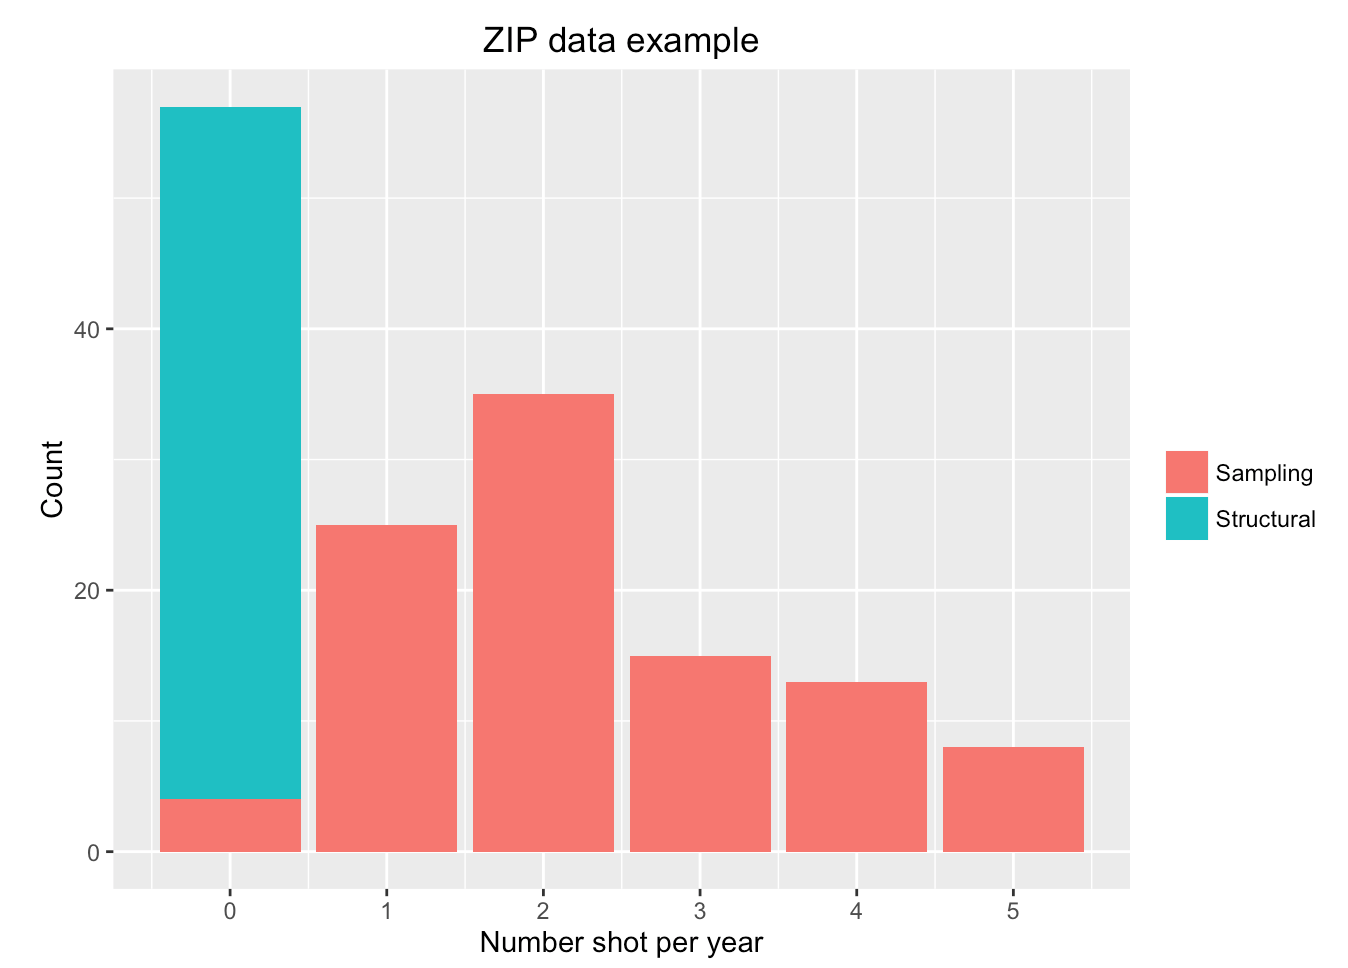
\includegraphics[width=0.6\textwidth]{figs/zip.png}
    \caption{Source: Zero-Inflated Models Statistics Honors Thesis Report Hope Johnson December 2016}
\end{figure}
\end{frame}



\begin{frame}{Zero-Inflated Regression Models}
\begin{itemize}
\item Zero-Inflated Regression Models are a combination of two parts:
\begin{enumerate}
\item A binary (logistic) model predicting whether an observation belongs to the "always-zero" group or the "not-necessarily-zero" group.
\item A count model (Poisson or Negative Binomial) for the non-zero observations.
\end{enumerate}
\item Each observation is modeled as potentially belonging to either of these two processes.
\end{itemize}
\end{frame}

\begin{frame}{Mathematical Representation}
Let's denote:
\begin{itemize}
\item $Y$ as the outcome variable,
\item $X$ as the predictor variables for the count part,
\item $W$ as the predictor variables for the binary part.
\end{itemize}
The Zero-Inflated Poisson (ZIP) model is formulated as follows:

$$
f\left(y \mid \pi, \mu\right)=\left\{\begin{array}{ll}\pi+(1-\pi) \operatorname{Poisson}(0 \mid \mu) & \text { if } y =0, \text { and } \\ (1-\pi)  \operatorname{Poisson}\left(y  \mid \mu\right) & \text { if } y >0\end{array}\right.
$$

where $\mu_i = \exp(\mathbf{x}_i^\top \boldsymbol{\beta})$ is the count mean and $\pi_i$ is the zero-inflation probability, modelled via logistic regression: $\operatorname{logit}(\pi_i) = \mathbf{w}_i^\top \boldsymbol{\gamma}$.

Similarly, a Zero-Inflated Negative Binomial (ZINB) model can be defined.
\end{frame}

\begin{frame}{Testing for zero-inflation}
\begin{itemize}
    \item van den Broek J (1995). ''A Score Test for Zero Inflation in a Poisson Distribution''. Biometrics, 51, 738–743.
    \item \texttt{countreg::zitest} -- Poisson only!
    \item Standard way: compare models with Log-Lik Ratio tests, BIC, AIC, cross-validation.
    \item Remember, the correct interpretation of results from zero-inflated models requires careful understanding of the two processes generating the data.
\end{itemize}
\end{frame}


\begin{frame}{Examples}

\end{frame}

\subsection{Hurdle models}

\begin{frame}{Introduction to Hurdle Models}
    \begin{figure}
        \centering
        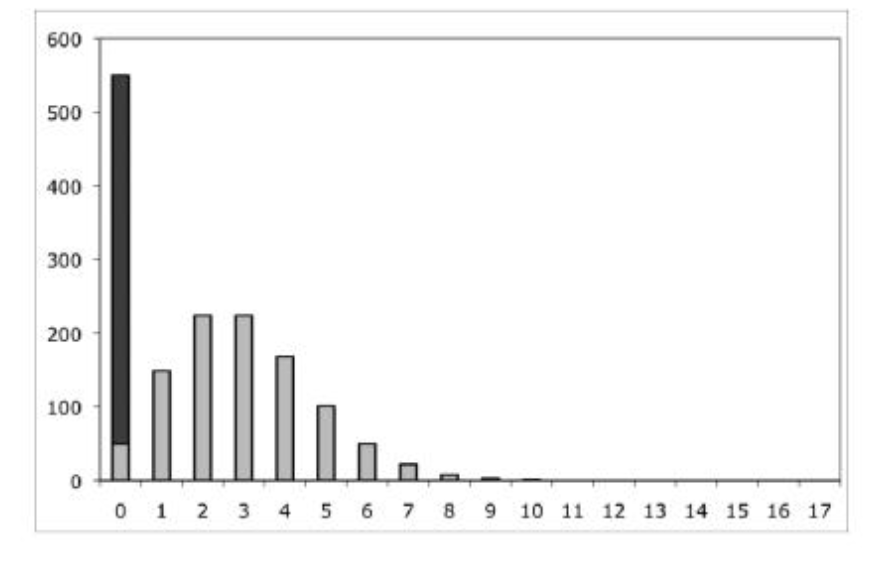
\includegraphics[width=0.45\textwidth]{figs/hur1.png}
        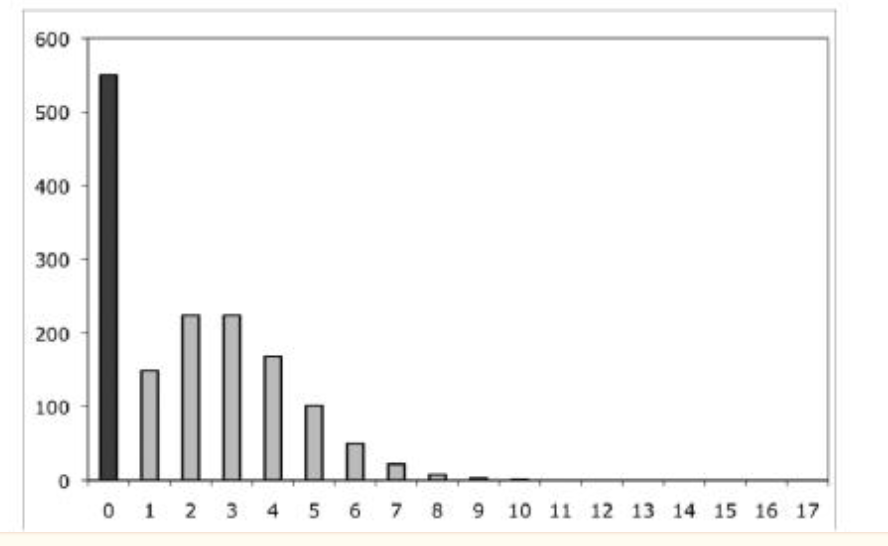
\includegraphics[width=0.45\textwidth]{figs/hur2.png}
        \caption{One-inflated (left) and hurdle (right) distribution. Based on Hu, M. C., Pavlicova, M., \& Nunes, E. V. (2011). Zero-inflated and hurdle models of count data with extra zeros: examples from an HIV-risk reduction intervention trial. The American journal of drug and alcohol abuse, 37(5), 367-375.}
    \end{figure}
\end{frame}


\begin{frame}{Introduction to Hurdle Models}
\begin{itemize}
\item Hurdle models are statistical models used to analyze data with excess zeros.
\item Similar to zero-inflated models, hurdle models address situations where zero outcomes are more frequent than expected.
\item Hurdle models use a two-component approach to tackle the excess zeros.
\item Hurdle models are commonly used when a large portion of the data contains zeros, but there is also a non-zero count component.
\item Example: 
\begin{itemize}
    \item You first decide if you need to buy something, and then you decide on the quantity of that something (which must be positive)
    \item Imagine you have data on the number of times users visit a particular website in a month. Many users might not visit the website at all, resulting in a large number of zeros. Among those who do visit the website, the number of visits might follow a different distribution. 
\end{itemize}. 
\end{itemize}
\end{frame}

\begin{frame}\frametitle{Understanding Excess Zeros}
\begin{itemize}
\item Excess zeros are observed when a substantial proportion of the data consists of zeros beyond what would be expected from a standard distribution.
\item In hurdle models, excess zeros are usually the result of a separate process from the count component.
\item The hurdle model uses two components, but \textbf{all zeros come from a single process} -- the binary hurdle. The (zero-truncated) count process generates only positive counts and cannot produce zeros. This contrasts with zero-inflated models, where zeros arise from \textbf{two} sources.
\end{itemize}
\end{frame}

\begin{frame}{Hurdle Model Components}
\begin{itemize}
\item Hurdle models consist of two components:
\begin{enumerate}
\item A binary model predicting the probability of observing a zero count (hurdle component).
\item A count model (Poisson or Negative Binomial) predicting the positive counts (count component).
\end{enumerate}
\item The binary model estimates the probability of belonging to the zero group, while the count model estimates the distribution of positive counts.
\item The hurdle component models the process of "getting over the hurdle" of zero counts, while the count component models the distribution of non-zero counts.
\end{itemize}
\end{frame}


\begin{frame}{Hurdle models}
  \begin{itemize}
      \item The hurdle model is similar to the zero-inflated model, but more flexible in that the zero outcomes can be deflated as well as inflated. 
      \item The probability mass function for the hurdle likelihood is defined by
      $$
f(y \mid \pi, \mu)=\left\{\begin{array}{ll}\pi & \text { if } y=0, \text { and } \\ (1-\pi) \frac{\text { Poisson }(y \mid \mu)}{1-\text { PoissonCDF }(0 \mid \mu)} & \text { if } y>0\end{array}\right.
$$
where \texttt{PoissonCDF} is the cumulative distribution function for the Poisson distribution, so $1-\operatorname{PoissonCDF}(0\mid\mu) = 1-e^{-\mu}$.
\item Extension: Here we assume that both models are independent, but in practice this may not be the case. Thus, hurdle models can be extended to selection models (allowing for correlation between y=0 and y>0 models).
  \end{itemize}  
\end{frame}

\begin{frame}{Zero-inflated vs hurdle models: recap}
\begin{itemize}
    \item \textbf{Zero-inflated (ZI) models} -- a \textbf{mixture} of two latent classes:
    \begin{itemize}
        \item A \textbf{structural} ``always-zero'' class (probability $\pi$): these units can \emph{never} produce a positive count.
        \item An \textbf{at-risk} class (probability $1-\pi$): units follow an ordinary (untruncated) Poisson/NB and may still record a zero.
        \item Zeros come from \textbf{two sources}: $P(Y=0) = \pi + (1-\pi)\,\mathrm{Poisson}(0\mid\mu)$.
    \end{itemize}
    \item \textbf{Hurdle models} -- a \textbf{two-part sequential} process:
    \begin{itemize}
        \item A \textbf{single binary gate} decides zero vs.\ positive (probability of zero $= \pi$).
        \item Conditional on crossing the hurdle ($Y>0$), counts follow a \textbf{zero-truncated} Poisson/NB (renormalized so zeros are impossible).
        \item \textbf{All zeros come from one source}: $P(Y=0) = \pi$.
    \end{itemize}
    \item \textbf{Key contrast:} ZI has zeros from \emph{two sources}, count part is \emph{untruncated}; hurdle has zeros from \emph{one source}, count part is \emph{zero-truncated}.
    \item \textbf{Practical note:} ZI models can only \emph{inflate} zeros; hurdle models can model both zero \emph{inflation} and zero \emph{deflation}.
\end{itemize}
\end{frame}

\begin{frame}{Hurdle vs zero-inflated Poisson models}
\begin{itemize}
    \item Zero-inflated models pmf/pdf

$$
f\left(y \mid \pi, \mu\right)=\left\{\begin{array}{ll}\pi+(1-\pi) \operatorname{Poisson}(0 \mid \mu) & \text { if } y=0, \text { and } \\ (1-\pi)  \operatorname{Poisson}\left(y \mid \mu\right) & \text { if } y>0\end{array}\right.
$$

    \item Hurdle models pmf/pdf

$$
f(y \mid \pi, \mu)=\left\{\begin{array}{ll}\pi & \text { if } y=0, \text { and } \\ (1-\pi) \frac{\text { Poisson }(y \mid \mu)}{1-\text { PoissonCDF }(0 \mid \mu)} & \text { if } y>0\end{array}\right.
$$
\end{itemize}

\end{frame}

\begin{frame}{Model selection}
\begin{itemize}
    \item Up to now we have discussed model selection based on information criteria (i.e., AIC, BIC) and rootograms.
    \item If we have selected the appropriate distribution, we can now work on variable selection (i.e., both models are fitted to the same distribution). For that purpose we can use the \textbf{Likelihood Ratio (LR) test} (alternatively Wald test).
    \begin{itemize}
        \item \textbf{Test Statistic:} $LR = -2[\ell_R - \ell_U] \sim \chi^2_{df}$
        \item \textbf{Degrees of Freedom:} $df = p_U - p_R$
    \end{itemize}
    \item Requirements:
    \begin{itemize}
        \item \textbf{Nested Models}: One model must be a special case of the other.
        \item \textbf{Same Data}: Both models fitted to identical observations.
        \item \textbf{Maximum Likelihood}: Both models estimated via ML.
        \item \textbf{Large Sample}: Asymptotic $\chi^2$ distribution assumption.
    \end{itemize}
\end{itemize}
\end{frame}


\begin{frame}{Model fit -- pseudo-$R^2$ for Count Models}

\textbf{What is pseudo-$R^2$?}

Traditional $R^2$ measures proportion of variance explained in linear regression. For count models (Poisson, Negative Binomial), we use maximum likelihood estimation, so we need alternative goodness-of-fit measures called pseudo $R^2$.

\vspace{0.1cm}

\textbf{Most Common: McFadden's Pseudo $R^2$}
$$R^2_{McFadden} = 1 - \frac{\ell(\hat{\beta})}{\ell_0}$$

where:
\begin{itemize}
\item $\ell(\hat{\beta})$ = log-likelihood of the fitted model
\item $\ell_0$ = log-likelihood of the intercept-only (null) model
\end{itemize}

\vspace{0.1cm}

\textbf{Interpretation:}
\begin{itemize}
\item Range: $[0, 1]$ with higher values indicating better fit
\item Values are typically much lower than OLS $R^2$
\item $R^2 > 0.20$ is considered excellent fit for count models
\end{itemize}

\end{frame}

\begin{frame}{Other pseudo-$R^2$ Measures}

\textbf{Cox-Snell pseudo-$R^2$}
$$R^2_{Cox-Snell} = 1 - \left(\frac{L_0}{L_1}\right)^{2/n}$$

\textbf{Nagelkerke pseudo-$R^2$} (adjusted Cox-Snell)
$$R^2_{Nagelkerke} = \frac{R^2_{Cox-Snell}}{1 - (L_0)^{2/n}}$$

\textbf{Cragg-Uhler pseudo-$R^2$}
$$R^2_{Cragg-Uhler} = \frac{1 - (L_0/L_1)^{2/n}}{1 - (L_0)^{2/n}}$$

\vspace{0.5cm}

where $L_0$ and $L_1$ are the likelihoods of null and fitted models, and $n$ is sample size.

\vspace{0.5cm}

\textbf{Note:} Different measures can give different values for the same model. McFadden's is most commonly reported.

\end{frame}


\begin{frame}[fragile]{An example R code (\texttt{pscl})}
\begin{small}
\begin{verbatim}
R> round(pscl::pR2(m1), 2)
fitting null model for pseudo-r2
       llh    llhNull         G2   McFadden       r2ML       r2CU 
-175507.42 -201143.48   51272.12       0.13       0.59       0.59 

R> round(pscl::pR2(m2), 2)
fitting null model for pseudo-r2
       llh    llhNull         G2   McFadden       r2ML       r2CU 
-161869.30 -201143.48   78548.35       0.20       0.75       0.75 

R> round(pscl::pR2(m3), 2)
fitting null model for pseudo-r2
       llh    llhNull         G2   McFadden       r2ML       r2CU 
-161838.47 -201143.48   78610.02       0.20       0.75       0.75 
\end{verbatim}  
\end{small}

\end{frame}

\begin{frame}[fragile]{An example R code (\texttt{performance})}
\begin{verbatim}
> library(performance)
> r2_mcfadden(m3)
# R2 for Generalized Linear Regression
       R2: 0.195
  adj. R2: 0.195

> r2_nagelkerke(m3)
Nagelkerke's R2 
      0.7462817 

> r2_coxsnell(m3)
Cox & Snell's R2 
       0.7452841 
\end{verbatim}
\end{frame}

\begin{frame}{Examples}

\end{frame}



\end{document}






